\chapter{Equivalent models of computation}\label{chapequivalentmodels}

\begin{objectives} \label[objectives]{Learn-about-RAM-machines-}

\begin{itemize}
\tightlist
\item
  Learn about RAM machines and the λ calculus.
\item
  Equivalence between these and other models and Turing machines.
\item
  Cellular automata and configurations of Turing machines.
\item
  Understand the Church-Turing thesis.
\end{itemize}

\end{objectives}

\begin{quote}
\emph{``All problems in computer science can be solved by another level
of indirection''}, attributed to David Wheeler.
\end{quote}

\begin{quote}
\emph{``Because we shall later compute with expressions for functions,
we need a distinction between functions and forms and a notation for
expressing this distinction. This distinction and a notation for
describing it, from which we deviate trivially, is given by Church.''},
John McCarthy, 1960 (in paper describing the LISP programming language)
\end{quote}

So far we have defined the notion of computing a function using Turing
machines, which are not a close match to the way computation is done in
practice. In this chapter we justify this choice by showing that the
definition of computable functions will remain the same under a wide
variety of computational models. This notion is known as \emph{Turing
completeness} or \emph{Turing equivalence} and is one of the most
fundamental facts of computer science. In fact, a widely believed claim
known as the \emph{Church-Turing Thesis} holds that \emph{every}
``reasonable'' definition of computable function is equivalent to being
computable by a Turing machine. We discuss the Church-Turing Thesis and
the potential definitions of ``reasonable'' in
\cref{churchturingdiscussionsec}.

Some of the main computational models we discuss in this chapter
include:

\begin{itemize}
\item
  \textbf{RAM Machines:} Turing Machines do not correspond to standard
  computing architectures that have \emph{Random Access Memory (RAM)}.
  The mathematical model of RAM machines is much closer to actual
  computers, but we will see that it is equivalent in power to Turing
  Machines. We also discuss a programming language variant of RAM
  machines, which we call NAND-RAM. The equivalence of Turing Machines
  and RAM machines enables demonstrating the \emph{Turing Equivalence}
  of many popular programming languages, including all general-purpose
  languages used in practice such as C, Python, JavaScript, etc.
\item
  \textbf{Cellular Automata:} Many natural and artificial systems can be
  modeled as collections of simple components, each evolving according
  to simple rules based on its state and the state of its immediate
  neighbors. One well-known such example is
  \href{https://en.wikipedia.org/wiki/Conway\%27s_Game_of_Life}{Conway's
  Game of Life}. To prove that cellular automata are equivalent to
  Turing machines we introduce the tool of \emph{configurations} of
  Turing Machines. These have other applications, and in particular are
  used in \cref{godelchap} to prove \emph{Gödel's Incompleteness
  Theorem}: a central result in mathematics.
\item
  \textbf{\(\lambda\) calculus:} The \(\lambda\) calculus is a model for
  expressing computation that originates from the 1930's, though it is
  closely connected to functional programming languages widely used
  today. Showing the equivalence of \(\lambda\) calculus to Turing
  Machines involves a beautiful technique to eliminate recursion known
  as the ``Y Combinator''.
\end{itemize}


\begin{figure}
\centering
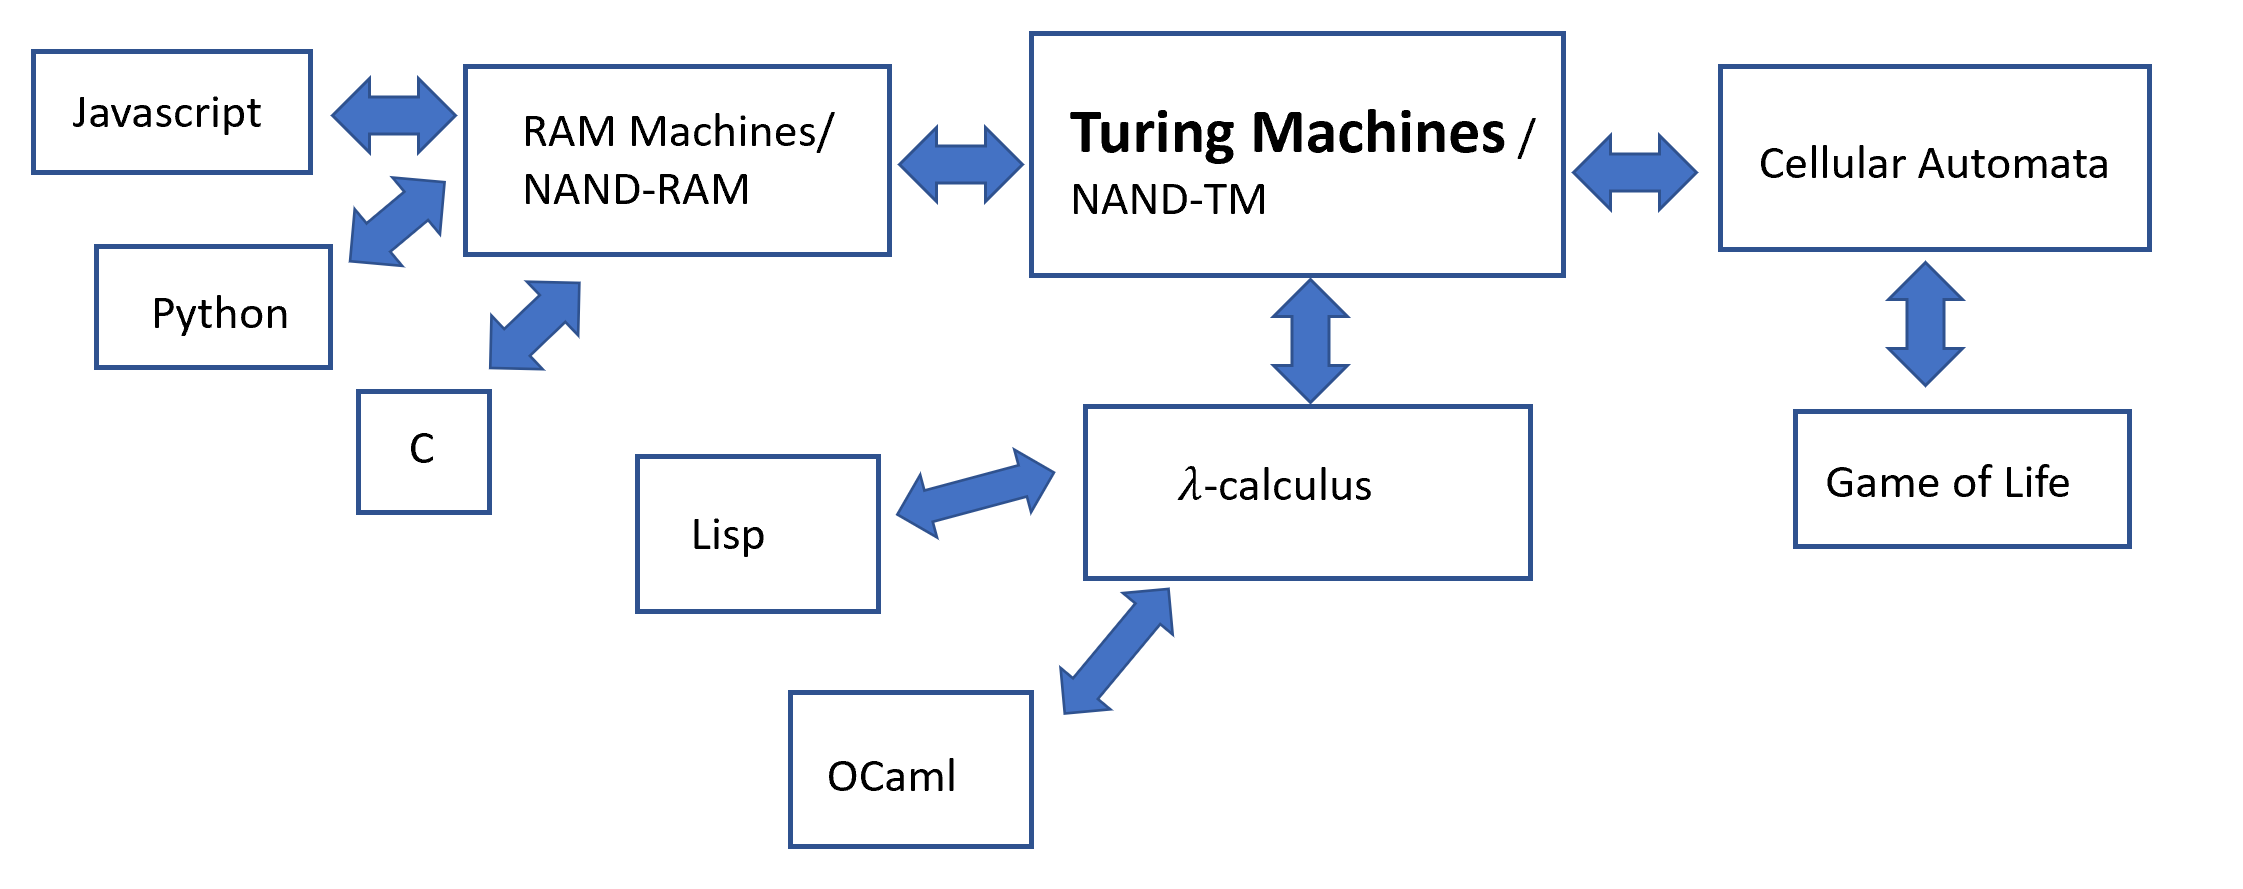
\includegraphics[width=\textwidth, height=0.25\paperheight, keepaspectratio]{../figure/turingcomplete.png}
\caption{Some Turing-equivalent models. All of these are equivalent in
power to Turing Machines (or equivalently NAND-TM programs) in the sense
that they can compute exactly the same class of functions. All of these
are models for computing \emph{infinite} functions that take inputs of
unbounded length. In contrast, Boolean circuits / NAND-CIRC programs can
only compute \emph{finite} functions and hence are not Turing complete.}
\label{turingcompletefig}
\end{figure}

\section{RAM machines and NAND-RAM}\label{RAM-machines-and-NAND-RAM}

One of the limitations of Turing Machines (and NAND-TM programs) is that
we can only access one location of our arrays/tape at a time. If the
head is at position \(22\) in the tape and we want to access the
\(957\)-th position then it will take us at least 923 steps to get
there. In contrast, almost every programming language has a formalism
for directly accessing memory locations. Actual physical computers also
provide so called \emph{Random Access Memory (RAM)} which can be thought
of as a large array \texttt{Memory}, such that given an index \(p\)
(i.e., memory address, or a \emph{pointer}), we can read from and write
to the \(p^{th}\) location of \texttt{Memory}. (``Random access memory''
is quite a misnomer since it has nothing to do with probability, but
since it is a standard term in both the theory and practice of
computing, we will use it as well.)

The computational model that models access to such a memory is the
\emph{RAM machine} (sometimes also known as the \emph{Word RAM model}),
as depicted in \cref{rammachinefig}. The memory of a RAM machine is an
array of unbounded size where each cell can store a single \emph{word},
which we think of as a string in \(\{0,1\}^w\) and also (equivalently)
as a number in \([2^w]\). For example, many modern computing
architectures use \(64\) bit words, in which every memory location holds
a string in \(\{0,1\}^{64}\) which can also be thought of as a number
between \(0\) and \(2^{64}-1= 9,223,372,036,854,775,807\). The parameter
\(w\) is known as the \emph{word size}. In practice often \(w\) is a
fixed number such as \(64\), but when doing theory we model \(w\) as a
parameter that can depend on the input length or number of steps. (You
can think of \(2^w\) as roughly corresponding to the largest memory
address that we use in the computation.) In addition to the memory
array, a RAM machine also contains a constant number of \emph{registers}
\(r_0,\ldots,r_{k-1}\), each of which can also contain a single word.


\begin{marginfigure}
\centering
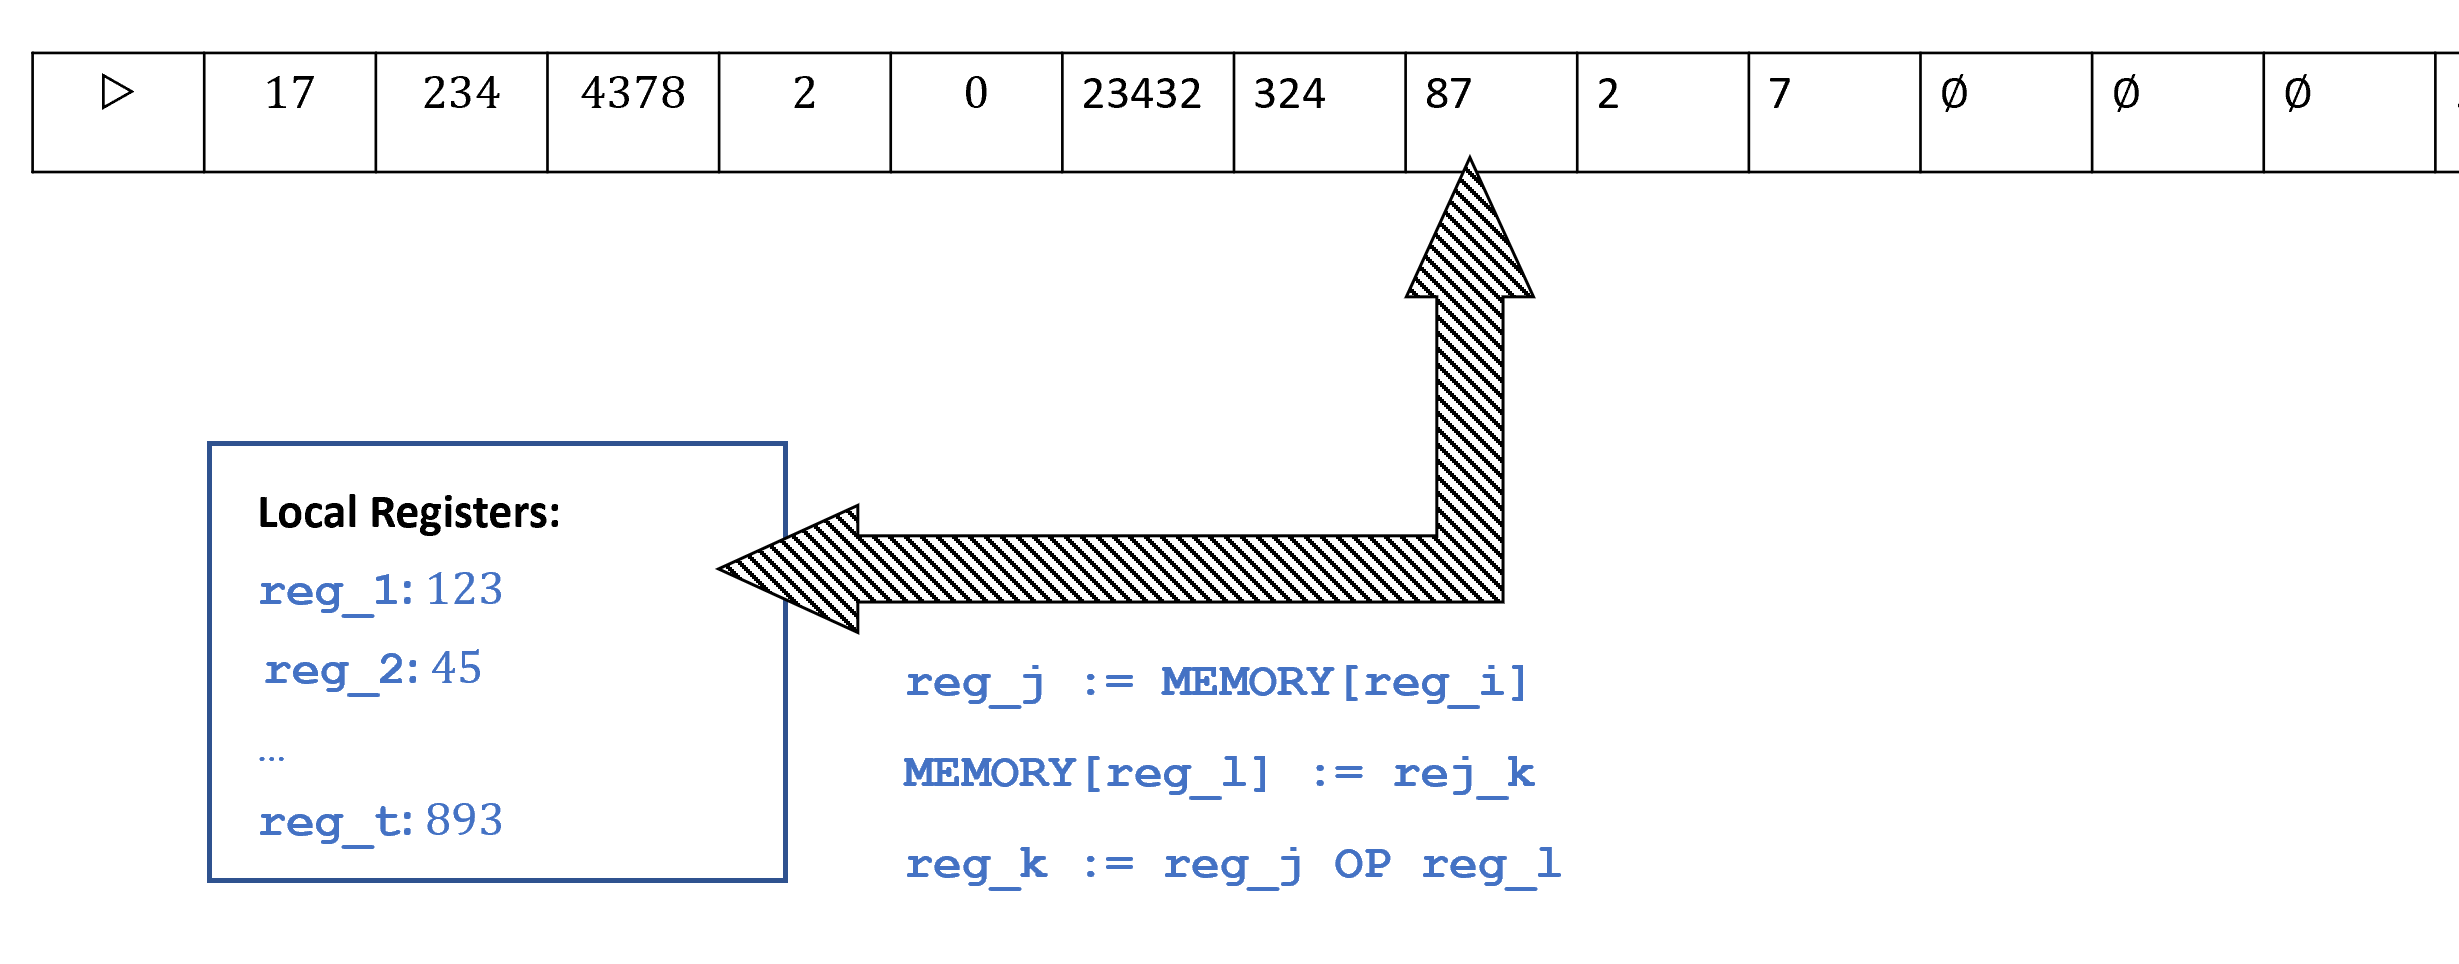
\includegraphics[width=\linewidth, height=1.5in, keepaspectratio]{../figure/rammachine.png}
\caption{A \emph{RAM Machine} contains a finite number of local
registers, each of which holds an integer, and an unbounded memory
array. It can perform arithmetic operations on its register as well as
load to a register \(r\) the contents of the memory at the address
indexed by the number in register \(r'\).}
\label{rammachinefig}
\end{marginfigure}

The operations a RAM machine can carry out include:

\begin{itemize}
\item
  \textbf{Data movement:} Load data from a certain cell in memory into a
  register or store the contents of a register into a certain cell of
  memory. RAM machine can directly access any cell of memory without
  having to move the ``head'' (as Turing machines do) to that location.
  That is, in one step a RAM machine can load into register \(r_i\) the
  contents of the memory cell indexed by register \(r_j\), or store into
  the memory cell indexed by register \(r_j\) the contents of register
  \(r_i\).
\item
  \textbf{Computation:} RAM machines can carry out computation on
  registers such as arithmetic operations, logical operations, and
  comparisons.
\item
  \textbf{Control flow:} As in the case of Turing machines, the choice
  of what instruction to perform next can depend on the state of the RAM
  machine, which is captured by the contents of its register.
\end{itemize}


\begin{marginfigure}
\centering
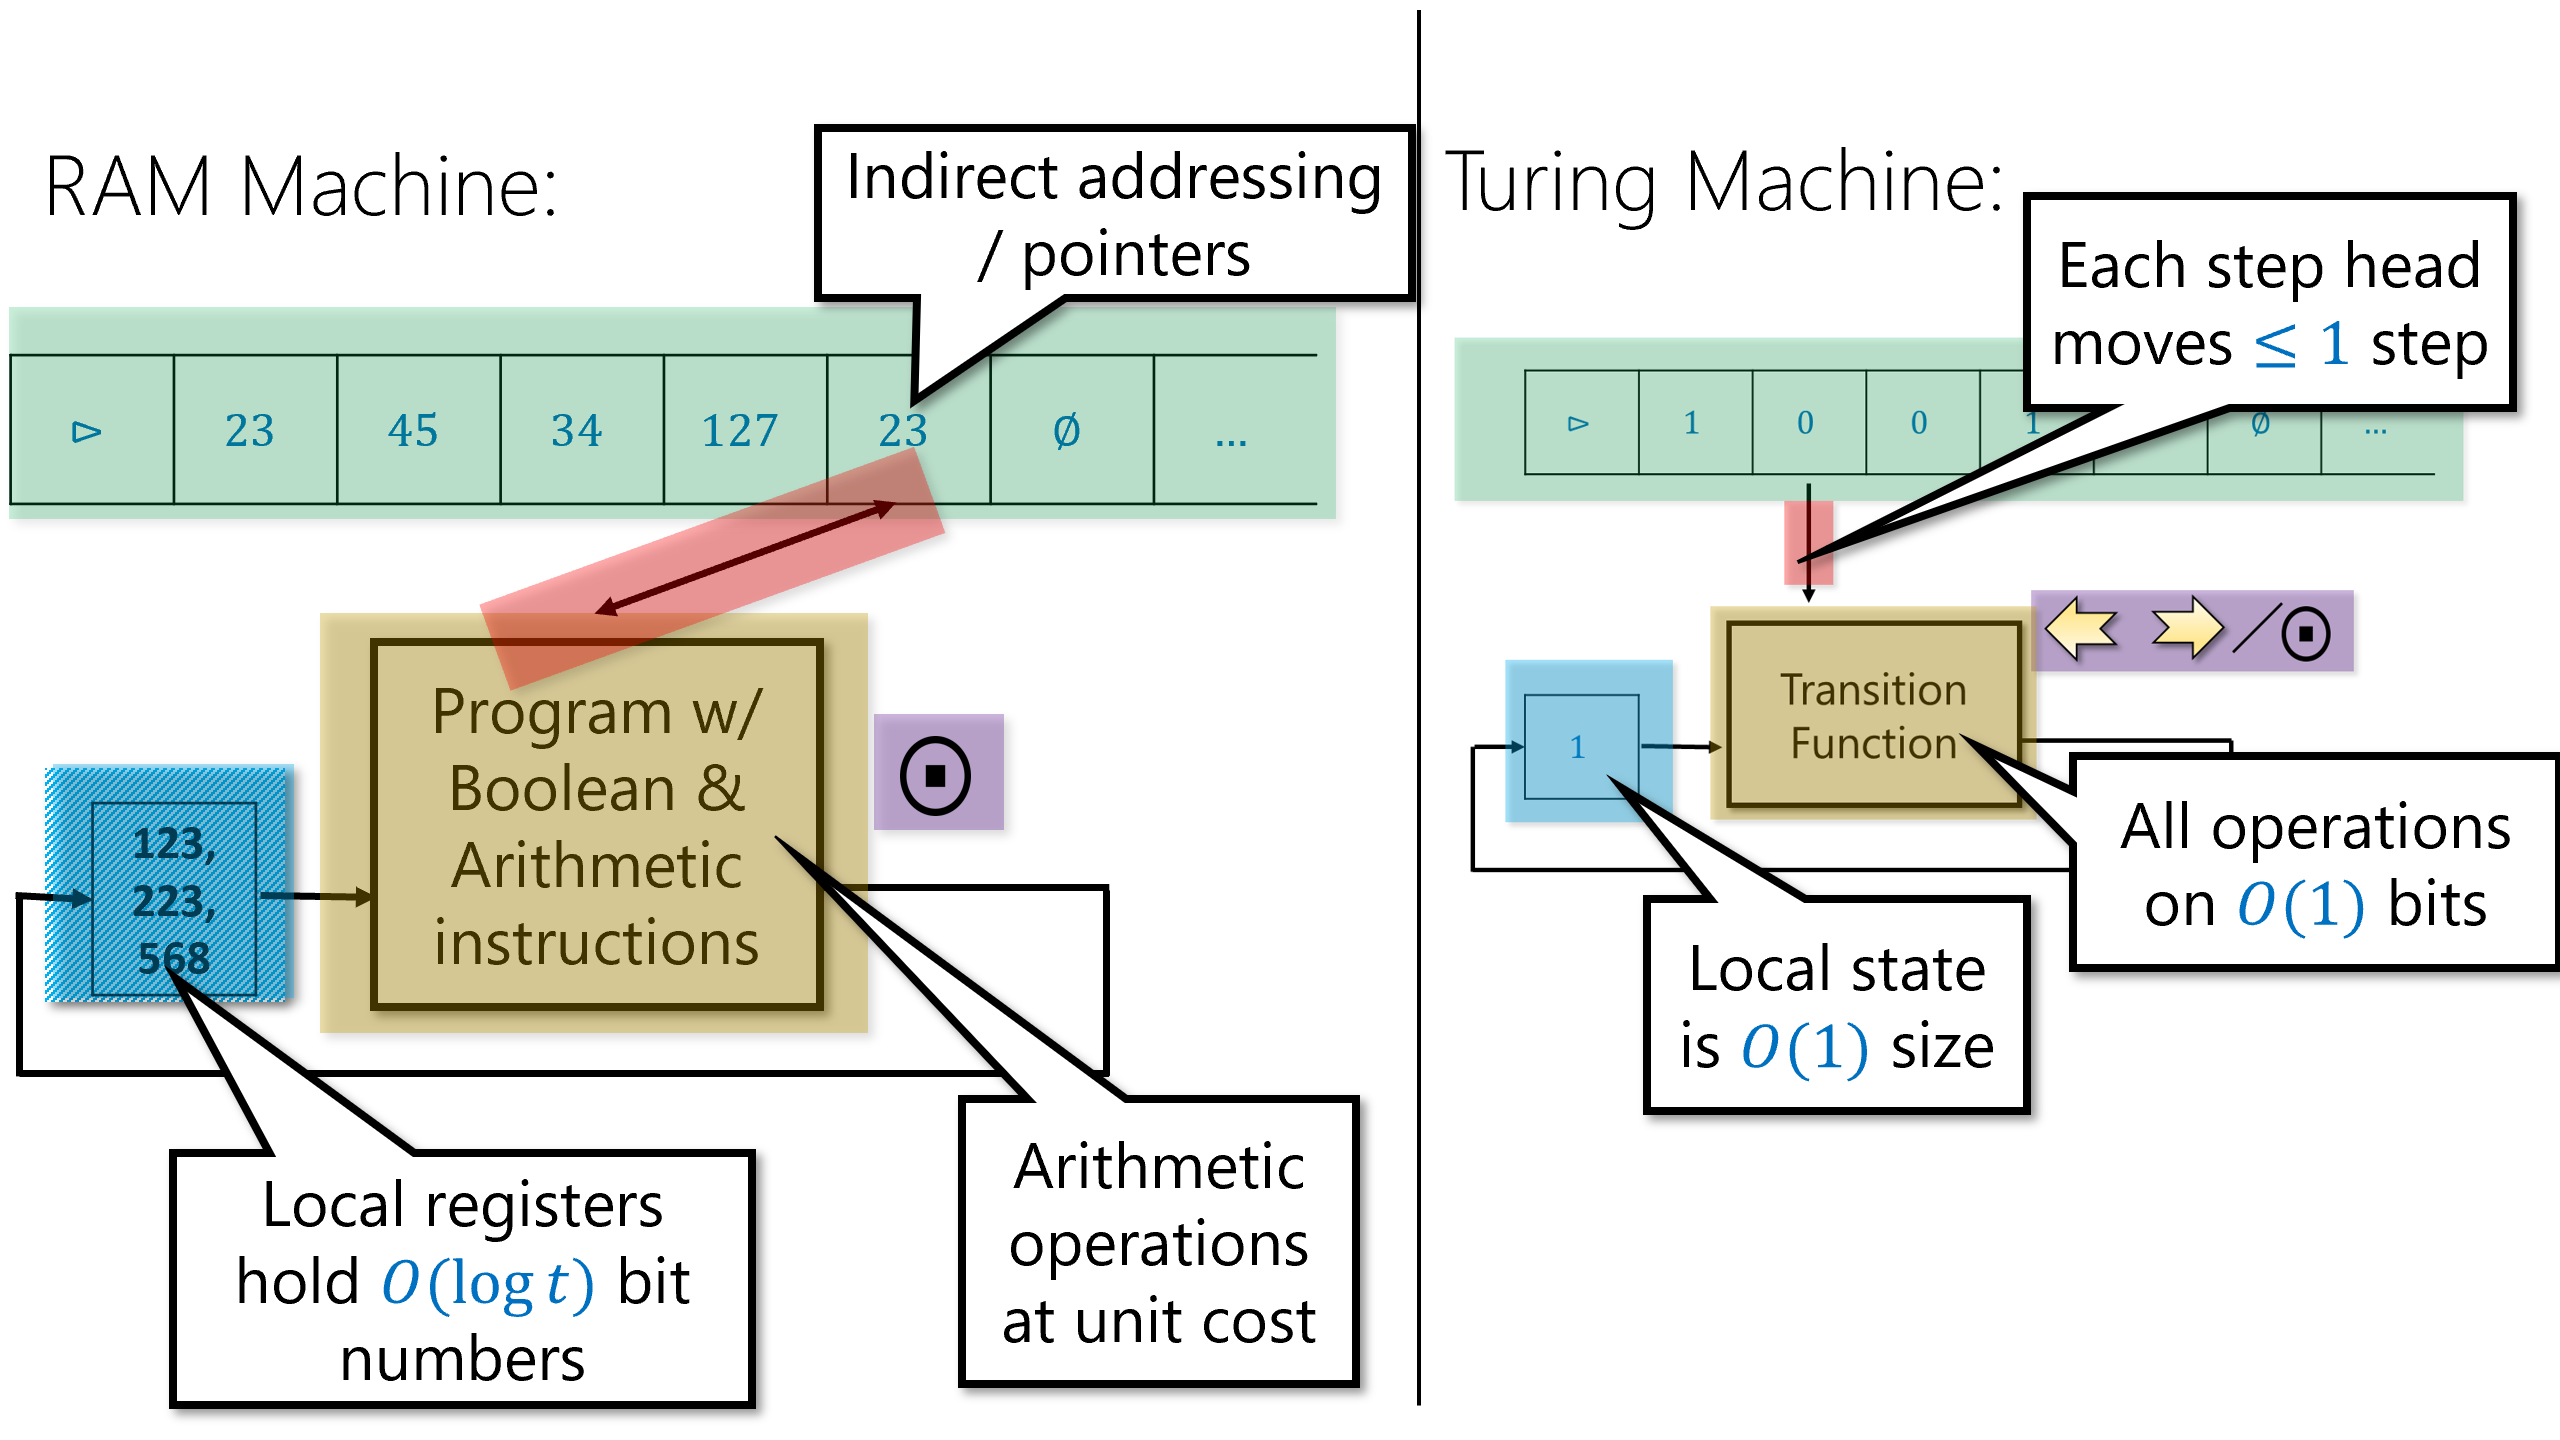
\includegraphics[width=\linewidth, height=1.5in, keepaspectratio]{../figure/ramvsturing.png}
\caption{Different aspects of RAM machines and Turing machines. RAM
machines can store integers in their local registers, and can read and
write to their memory at a location specified by a register. In
contrast, Turing machines can only access their memory in the head
location, which moves at most one position to the right or left in each
step.}
\label{ramvsturingfig}
\end{marginfigure}

We will not give a formal definition of RAM Machines, though the
bibliographical notes section (\cref{othermodelsbibnotes}) contains
sources for such definitions. Just as the NAND-TM programming language
models Turing machines, we can also define a \emph{NAND-RAM programming
language} that models RAM machines. The NAND-RAM programming language
extends NAND-TM by adding the following features:

\begin{itemize}
\item
  The variables of NAND-RAM are allowed to be (non negative)
  \emph{integer valued} rather than only Boolean as is the case in
  NAND-TM. That is, a scalar variable \texttt{foo} holds a non negative
  integer in \(\N\) (rather than only a bit in \(\{0,1\}\)), and an
  array variable \texttt{Bar} holds an array of integers. As in the case
  of RAM machines, we will not allow integers of unbounded size.
  Concretely, each variable holds a number between \(0\) and \(T-1\),
  where \(T\) is the number of steps that have been executed by the
  program so far. (You can ignore this restriction for now: if we want
  to hold larger numbers, we can simply execute dummy instructions; it
  will be useful in later chapters.)
\item
  We allow \emph{indexed access} to arrays. If \texttt{foo} is a scalar
  and \texttt{Bar} is an array, then \texttt{Bar[foo]} refers to the
  location of \texttt{Bar} indexed by the value of \texttt{foo}. (Note
  that this means we don't need to have a special index variable
  \texttt{i} any more.)
\item
  As is often the case in programming languages, we will assume that for
  Boolean operations such as \texttt{NAND}, a zero valued integer is
  considered as \emph{false}, and a nonzero valued integer is considered
  as \emph{true}.
\item
  In addition to \texttt{NAND}, NAND-RAM also includes all the basic
  arithmetic operations of addition, subtraction, multiplication,
  (integer) division, as well as comparisons (equal, greater than, less
  than, etc..).
\item
  NAND-RAM includes conditional statements \texttt{if}/\texttt{then} as
  part of the language.
\item
  NAND-RAM contains looping constructs such as \texttt{while} and
  \texttt{do} as part of the language.
\end{itemize}

A full description of the NAND-RAM programming language is in the
\href{http://tiny.cc/introtcsappendix}{appendix}. However, the most
important fact you need to know about NAND-RAM is that you actually
don't need to know much about NAND-RAM at all, since it is equivalent in
power to Turing machines:

\hypertarget{RAMTMequivalencethm}{}
\begin{theorem}[Turing Machines (aka NAND-TM programs) and RAM machines (aka NAND-RAM programs) are equivalent] \label[theorem]{RAMTMequivalencethm}

For every function \(F:\{0,1\}^* \rightarrow \{0,1\}^*\), \(F\) is
computable by a NAND-TM program if and only if \(F\) is computable by a
NAND-RAM program.

\end{theorem}

Since NAND-TM programs are equivalent to Turing machines, and NAND-RAM
programs are equivalent to RAM machines, \cref{RAMTMequivalencethm}
shows that all these four models are equivalent to one another.


\begin{marginfigure}
\centering
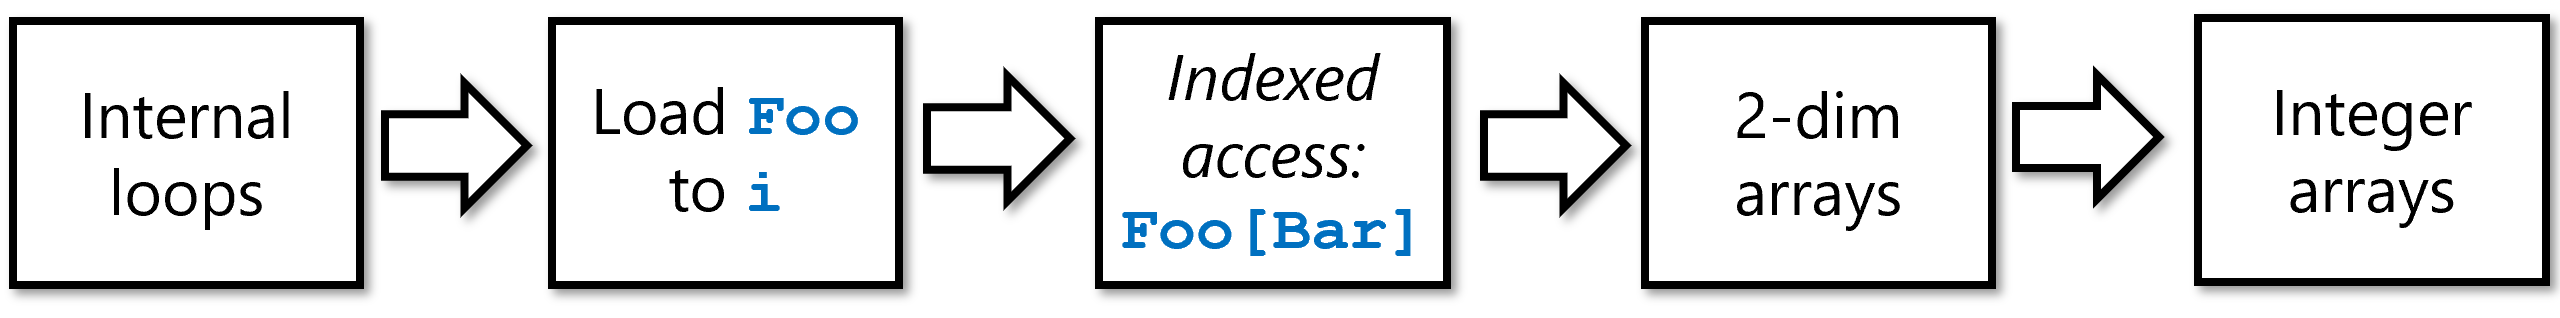
\includegraphics[width=\linewidth, height=1.5in, keepaspectratio]{../figure/nandramproofoverview.png}
\caption{Overview of the steps in the proof of
\cref{RAMTMequivalencethm} simulating NANDRAM with NANDTM. We first use
the inner loop syntactic sugar of \cref{nandtminnerloopssec} to enable
loading an integer from an array to the index variable \texttt{i} of
NANDTM. Once we can do that, we can simulate \emph{indexed access} in
NANDTM. We then use an embedding of \(\N^2\) in \(\N\) to simulate two
dimensional bit arrays in NANDTM. Finally, we use the binary
representation to encode one-dimensional arrays of integers as two
dimensional arrays of bits hence completing the simulation of NANDRAM
with NANDTM.}
\label{nandramoverviewfig}
\end{marginfigure}

\begin{proofidea} \label[proofidea]{Clearly-NAND-RAM-is-only-}

Clearly NAND-RAM is only more powerful than NAND-TM, and so if a
function \(F\) is computable by a NAND-TM program then it can be
computed by a NAND-RAM program. The challenging direction is to
transform a NAND-RAM program \(P\) to an equivalent NAND-TM program
\(Q\). To describe the proof in full we will need to cover the full
formal specification of the NAND-RAM language, and show how we can
implement every one of its features as syntactic sugar on top of
NAND-TM.

This can be done but going over all the operations in detail is rather
tedious. Hence we will focus on describing the main ideas behind this
transformation. (See also \cref{nandramoverviewfig}.) NAND-RAM
generalizes NAND-TM in two main ways: \textbf{(a)} adding \emph{indexed
access} to the arrays (ie.., \texttt{Foo[bar]} syntax) and \textbf{(b)}
moving from \emph{Boolean valued} variables to \emph{integer valued}
ones. The transformation has two steps:

\begin{enumerate}
\def\labelenumi{\arabic{enumi}.}
\item
  \emph{Indexed access of bit arrays:} We start by showing how to handle
  \textbf{(a)}. Namely, we show how we can implement in NAND-TM the
  operation \texttt{Setindex(Bar)} such that if \texttt{Bar} is an array
  that encodes some integer \(j\), then after executing
  \texttt{Setindex(Bar)} the value of \texttt{i} will equal to \(j\).
  This will allow us to simulate syntax of the form \texttt{Foo[Bar]} by
  \texttt{Setindex(Bar)} followed by \texttt{Foo[i]}.
\item
  \emph{Two dimensional bit arrays:} We then show how we can use
  ``syntactic sugar'' to augment NAND-TM with \emph{two dimensional
  arrays}. That is, have \emph{two indices} \texttt{i} and \texttt{j}
  and \emph{two dimensional arrays}, such that we can use the syntax
  \texttt{Foo[i][j]} to access the (\texttt{i},\texttt{j})-th location
  of \texttt{Foo}.
\item
  \emph{Arrays of integers:} Finally we will encode a one dimensional
  array \texttt{Arr} of \emph{integers} by a two dimensional
  \texttt{Arrbin} of \emph{bits}. The idea is simple: if
  \(a_{i,0},\ldots,a_{i,\ell}\) is a binary (prefix-free) representation
  of \texttt{Arr[}\(i\)\texttt{]}, then
  \texttt{Arrbin[}\(i\)\texttt{][}\(j\)\texttt{]} will be equal to
  \(a_{i,j}\).
\end{enumerate}

Once we have arrays of integers, we can use our usual syntactic sugar
for functions, \texttt{GOTO} etc. to implement the arithmetic and
control flow operations of NAND-RAM.

\end{proofidea}

The above approach is not the only way to obtain a proof of
\cref{RAMTMequivalencethm}, see for example \cref{RAMTMalternativeex}

\hypertarget{NANDRAMassembly}{}
\begin{remark}[RAM machines / NAND-RAM and assembly language (optional)] \label[remark]{NANDRAMassembly}

RAM machines correspond quite closely to actual microprocessors such as
those in the Intel x86 series that also contains a large \emph{primary
memory} and a constant number of small registers. This is of course no
accident: RAM machines aim at modeling more closely than Turing machines
the architecture of actual computing systems, which largely follows the
so called
\href{https://en.wikipedia.org/wiki/Von_Neumann_architecture}{von
Neumann architecture} as described in the report \cite{vonNeumann45}. As
a result, NAND-RAM is similar in its general outline to assembly
languages such as x86 or NIPS. These assembly languages all have
instructions to \textbf{(1)} move data from registers to memory,
\textbf{(2)} perform arithmetic or logical computations on registers,
and \textbf{(3)} conditional execution and loops (``if'' and ``goto'',
commonly known as ``branches'' and ``jumps'' in the context of assembly
languages).

The main difference between RAM machines and actual microprocessors (and
correspondingly between NAND-RAM and assembly languages) is that actual
microprocessors have a fixed word size \(w\) so that all registers and
memory cells hold numbers in \([2^w]\) (or equivalently strings in
\(\{0,1\}^w\)). This number \(w\) can vary among different processors,
but common values are either \(32\) or \(64\). As a theoretical model,
RAM machines do not have this limitation, but we rather let \(w\) be the
logarithm of our running time (which roughly corresponds to its value in
practice as well). Actual microprocessors also have a fixed number of
registers (e.g., 14 general purpose registers in x86-64) but this does
not make a big difference with RAM machines. It can be shown that RAM
machines with as few as two registers are as powerful as full-fledged
RAM machines that have an arbitrarily large constant number of
registers.

Of course actual microprocessors have many features not shared with RAM
machines as well, including parallelism, memory hierarchies, and many
others. However, RAM machines do capture actual computers to a first
approximation and so (as we will see), the running time of an algorithm
on a RAM machine (e.g., \(O(n)\) vs \(O(n^2)\)) is strongly correlated
with its practical efficiency.

\end{remark}

\section{The gory details (optional)}\label{nandtmgorydetailssec}

We do not show the full formal proof of \cref{RAMTMequivalencethm} but
focus on the most important parts: implementing indexed access, and
simulating two dimensional arrays with one dimensional ones. Even these
are already quite tedious to describe, as will not be surprising to
anyone that has ever written a compiler. Hence you can feel free to
merely skim this section. The important point is not for you to know all
details by heart but to be convinced that in principle it \emph{is}
possible to transform a NAND-RAM program to an equivalent NAND-TM
program, and even be convinced that, with sufficient time and effort,
\emph{you} could do it if you wanted to.

\subsection{Indexed access in NAND-TM}\label{Indexed-access-in-NAND-TM}

In NAND-TM we can only access our arrays in the position of the index
variable \texttt{i}, while NAND-RAM has integer-valued variables and can
use them for \emph{indexed access} to arrays, of the form
\texttt{Foo[bar]}. To implement indexed access in NAND-TM, we will
encode integers in our arrays using some prefix-free representation (see
\cref{prefixfreesec})), and then have a procedure \texttt{Setindex(Bar)}
that sets \texttt{i} to the value encoded by \texttt{Bar}. We can
simulate the effect of \texttt{Foo[Bar]} using \texttt{Setindex(Bar)}
followed by \texttt{Foo[i]}.

Implementing \texttt{Setindex(Bar)} can be achieved as follows:

\begin{enumerate}
\def\labelenumi{\arabic{enumi}.}
\item
  We initialize an array \texttt{Arzero} such that
  \texttt{Atzero[}\(0\)\texttt{]}\(=1\) and
  \texttt{Atzero[}\(j\)\texttt{]}\(=0\) for all \(j>0\). (This can be
  easily done in NAND-TM as all uninitialized variables default to
  zero.)
\item
  Set \texttt{i} to zero, by decrementing it until we reach the point
  where \texttt{Atzero[i]}\(=1\).
\item
  Let \texttt{Temp} be an array encoding the number \(0\).
\item
  We use \texttt{GOTO} to simulate an inner loop of of the form:
  \textbf{while} \texttt{Temp} \(\neq\) \texttt{Bar}, increment
  \texttt{Temp}.
\item
  At the end of the loop, \texttt{i} is equal to the value encoded by
  \texttt{Bar}.
\end{enumerate}

In NAND-TM code (using some syntactic sugar), we can implement the above
operations as follows:

\begin{code}
# assume Atzero is an array such that Atzero[0]=1
# and Atzero[j]=0 for all j>0

# set i to 0.
LABEL("zero_idx")
dir0 = zero
dir1 = one
# corresponds to i <- i-1
GOTO("zero_idx",NOT(Atzero[i]))
...
# zero out temp
#(code below assumes a specific prefix-free encoding in which 10 is the "end marker")
Temp[0] = 1
Temp[1] = 0
# set i to Bar, assume we know how to increment, compare
LABEL("increment_temp")
cond = EQUAL(Temp,Bar)
dir0 = one
dir1 = one
# corresponds to i <- i+1
INC(Temp)
GOTO("increment_temp",cond)
# if we reach this point, i is number encoded by Bar
...
# final instruction of program
MODANDJUMP(dir0,dir1)
\end{code}

\subsection{Two dimensional arrays in
NAND-TM}\label{Two-dimensional-arrays-in}

To implement two dimensional arrays, we want to embed them in a one
dimensional array. The idea is that we come up with a \emph{one to one}
function \(embed:\N \times \N \rightarrow \N\), and so embed the
location \((i,j)\) of the two dimensional array \texttt{Two} in the
location \(embed(i,j)\) of the array \texttt{One}.

Since the set \(\N \times \N\) seems ``much bigger'' than the set
\(\N\), a priori it might not be clear that such a one to one mapping
exists. However, once you think about it more, it is not that hard to
construct. For example, you could ask a child to use scissors and glue
to transform a 10" by 10" piece of paper into a 1" by 100" strip. This
is essentially a one to one map from \([10]\times [10]\) to \([100]\).
We can generalize this to obtain a one to one map from \([n]\times [n]\)
to \([n^2]\) and more generally a one to one map from \(\N \times \N\)
to \(\N\). Specifically, the following map \(embed\) would do (see
\cref{pairingfuncfig}):

\[embed(x,y) = \tfrac{1}{2}(x+y)(x+y+1)+x\;\;.\]


\begin{marginfigure}
\centering
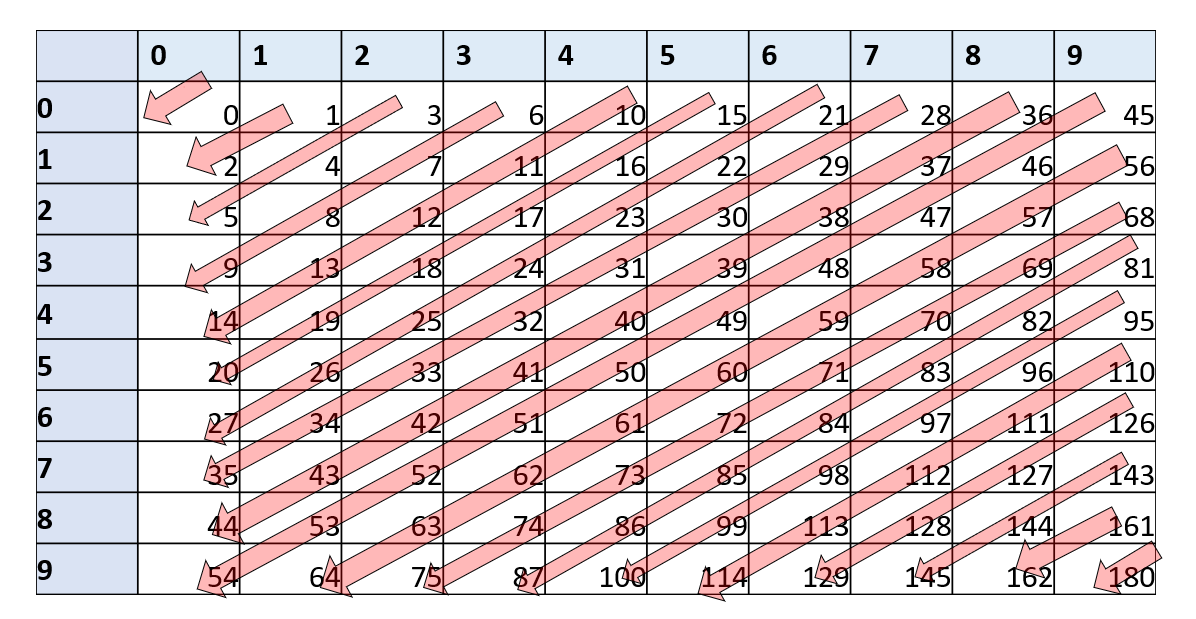
\includegraphics[width=\linewidth, height=1.5in, keepaspectratio]{../figure/pairing_function.png}
\caption{Illustration of the map
\(embed(x,y) = \tfrac{1}{2}(x+y)(x+y+1)+x\) for \(x,y \in [10]\), one
can see that for every distinct pairs \((x,y)\) and \((x',y')\),
\(embed(x,y) \neq embed(x',y')\).}
\label{pairingfuncfig}
\end{marginfigure}

\cref{pair-ex} asks you to prove that \(embed\) is indeed one to one, as
well as computable by a NAND-TM program. (The latter can be done by
simply following the grade-school algorithms for multiplication,
addition, and division.) This means that we can replace code of the form
\texttt{Two[Foo][Bar] = something} (i.e., access the two dimensional
array \texttt{Two} at the integers encoded by the one dimensional arrays
\texttt{Foo} and \texttt{Bar}) by code of the form:

\begin{code}
Blah = embed(Foo,Bar)
Setindex(Blah)
Two[i] = something
\end{code}

\subsection{All the rest}\label{All-the-rest}

Once we have two dimensional arrays and indexed access, simulating
NAND-RAM with NAND-TM is just a matter of implementing the standard
algorithms for arithmetic operations and comparisons in NAND-TM. While
this is cumbersome, it is not difficult, and the end result is to show
that every NAND-RAM program \(P\) can be simulated by an equivalent
NAND-TM program \(Q\), thus completing the proof of
\cref{RAMTMequivalencethm}.

\hypertarget{recursion}{}
\begin{remark}[Recursion in NAND-RAM (advanced)] \label[remark]{recursion}

One concept that appears in many programming languages but we did not
include in NAND-RAM programs is \emph{recursion}. However, recursion
(and function calls in general) can be implemented in NAND-RAM using the
\href{https://goo.gl/JweMj}{stack data structure}. A \emph{stack} is a
data structure containing a sequence of elements, where we can ``push''
elements into it and ``pop'' them from it in ``first in last out''
order.

We can implement a stack using an array of integers \texttt{Stack} and a
scalar variable \texttt{stackpointer} that will be the number of items
in the stack. We implement \texttt{push(foo)} by

\begin{code}
Stack[stackpointer]=foo
stackpointer += one
\end{code}

and implement \texttt{bar = pop()} by

\begin{code}
bar = Stack[stackpointer]
stackpointer -= one
\end{code}

We implement a function call to \(F\) by pushing the arguments for \(F\)
into the stack. The code of \(F\) will ``pop'' the arguments from the
stack, perform the computation (which might involve making recursive or
non recursive calls) and then ``push'' its return value into the stack.
Because of the ``first in last out'' nature of a stack, we do not return
control to the calling procedure until all the recursive calls are done.

The fact that we can implement recursion using a non-recursive language
is not surprising. Indeed, \emph{machine languages} typically do not
have recursion (or function calls in general), and hence a compiler
implements function calls using a stack and \texttt{GOTO}. You can find
online tutorials on how recursion is implemented via stack in your
favorite programming language, whether it's
\href{http://interactivepython.org/runestone/static/pythonds/Recursion/StackFramesImplementingRecursion.html}{Python}
, \href{https://javascript.info/recursion}{JavaScript}, or
\href{https://mitpress.mit.edu/sicp/full-text/sicp/book/node110.html}{Lisp/Scheme}.

\end{remark}

\section{Turing equivalence
(discussion)}\label{Turing-equivalence-discus}


\begin{marginfigure}
\centering
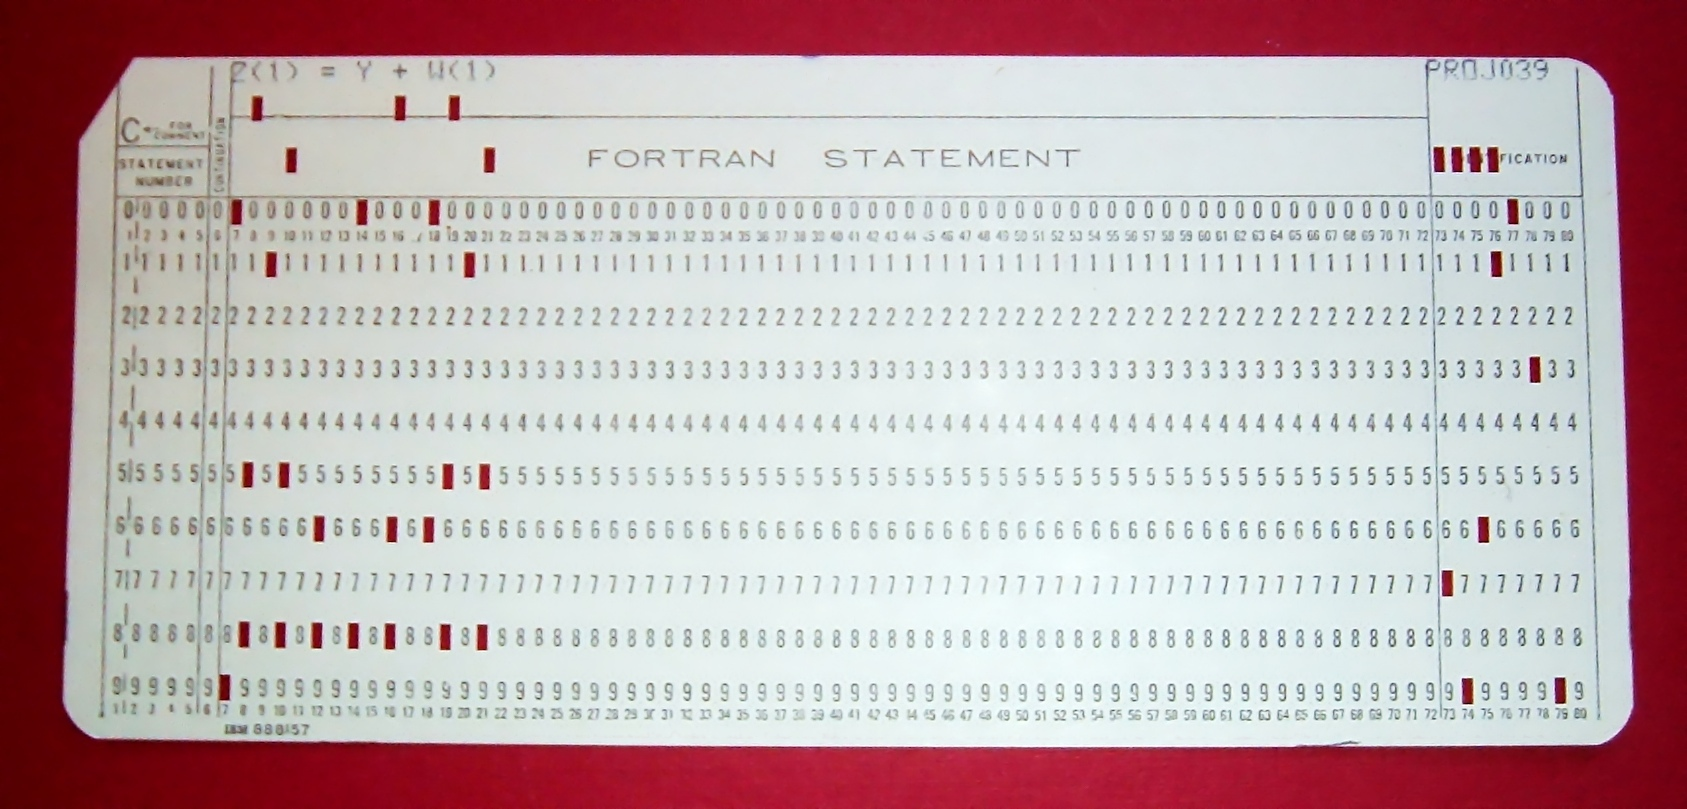
\includegraphics[width=\linewidth, height=1.5in, keepaspectratio]{../figure/FortranProg.jpg}
\caption{A punched card corresponding to a Fortran statement.}
\label{fortranfig}
\end{marginfigure}

Any of the standard programming language such as \texttt{C},
\texttt{Java}, \texttt{Python}, \texttt{Pascal}, \texttt{Fortran} have
very similar operations to NAND-RAM. (Indeed, ultimately they can all be
executed by machines which have a fixed number of registers and a large
memory array.) Hence using \cref{RAMTMequivalencethm}, we can simulate
any program in such a programming language by a NAND-TM program. In the
other direction, it is a fairly easy programming exercise to write an
interpreter for NAND-TM in any of the above programming languages. Hence
we can also simulate NAND-TM programs (and so by \cref{TM-equiv-thm},
Turing machines) using these programming languages. This property of
being equivalent in power to Turing Machines / NAND-TM is called
\emph{Turing Equivalent} (or sometimes \emph{Turing Complete}). Thus all
programming languages we are familiar with are Turing
equivalent.\footnote{Some programming language have fixed (even if
  extremely large) bounds on the amount of memory they can access, which
  formally prevent them from being applicable to computing infinite
  functions and hence simulating Turing machines. We ignore such issues
  in this discussion and assume access to some storage device without a
  fixed upper bound on its capacity.}

\subsection{The ``Best of both worlds''
paradigm}\label{The-Best-of-both-worlds-p}

The equivalence between Turing Machines and RAM machines allows us to
choose the most convenient language for the task at hand:

\begin{itemize}
\item
  When we want to \emph{prove a theorem} about all programs/algorithms,
  we can use Turing machines (or NAND-TM) since they are simpler and
  easier to analyze. In particular, if we want to show that a certain
  function \emph{can not} be computed, then we will use Turing machines.
\item
  When we want to show that a function \emph{can be computed} we can use
  RAM machines or NAND-RAM, because they are easier to program in and
  correspond more closely to high level programming languages we are
  used to. In fact, we will often describe NAND-RAM programs in an
  informal manner, trusting that the reader can fill in the details and
  translate the high level description to the precise program. (This is
  just like the way people typically use informal or ``pseudocode''
  descriptions of algorithms, trusting that their audience will know to
  translate these descriptions to code if needed.)
\end{itemize}

Our usage of Turing Machines / NAND-TM and RAM Machines / NAND-RAM is
very similar to the way people use in practice high and low level
programming languages. When one wants to produce a device that executes
programs, it is convenient to do so for very simple and ``low level''
programming language. When one wants to describe an algorithm, it is
convenient to use as high level a formalism as possible.


\begin{marginfigure}
\centering

\includegraphics[width=\linewidth, height=1.5in, keepaspectratio]{../figure/have_your_cake_and_eat_it_too-img-intro.png}
\caption{By having the two equivalent languages NAND-TM and NAND-RAM, we
can ``have our cake and eat it too'', using NAND-TM when we want to
prove that programs \emph{can't} do something, and using NAND-RAM or
other high level languages when we want to prove that programs
\emph{can} do something.}
\label{cakefig}
\end{marginfigure}

\hypertarget{eatandhavecake}{}
\begin{bigidea} \label[bigidea]{eatandhavecake}

Using equivalence results such as those between Turing and RAM machines,
we can \emph{``have our cake and eat it too''}.

We can use a simpler model such as Turing machines when we want to prove
something \emph{can't} be done, and use a feature-rich model such as RAM
machines when we want to prove something \emph{can} be done.

\end{bigidea}

\subsection{Let's talk about
abstractions.}\label{Lets-talk-about-abstracti}

\begin{quote}
``The programmer is in the unique position that \ldots{} he has to be
able to think in terms of conceptual hierarchies that are much deeper
than a single mind ever needed to face before.'', Edsger Dijkstra, ``On
the cruelty of really teaching computing science'', 1988.
\end{quote}

At some point in any theory of computation course, the instructor and
students need to have \emph{the talk}. That is, we need to discuss the
\emph{level of abstraction} in describing algorithms. In algorithms
courses, one typically describes algorithms in English, assuming readers
can ``fill in the details'' and would be able to convert such an
algorithm into an implementation if needed. For example,
\cref{bfsalghighlevel} is a high level description of the
\href{https://goo.gl/ug7Jaj}{breadth first search} algorithm.

\begin{algorithm}[Breadth First Search]
\label[algorithm]{bfsalghighlevel} ~ \\ \noindent
\begin{algorithmic}[1]
\INPUT  Graph $G$, vertices $u,v$
\OUTPUT  "connected" when $u$ is connected to $v$ in $G$, "disconnected"
\STATE Initialize empty queue $Q$.
\STATE Put $u$ in $Q$
\WHILE{$Q$ is not empty}
   \STATE Remove top vertex $w$ from $Q$
   \IF{$w=v$} \RETURN "connected" \ENDIF
   \STATE Mark $w$
   \STATE Add all unmarked neighbors of $w$ to $Q$.
\ENDWHILE
\RETURN "disconnected"
\end{algorithmic}
\end{algorithm}

If we wanted to give more details on how to implement breadth first
search in a programming language such as Python or C (or NAND-RAM /
NAND-TM for that matter), we would describe how we implement the queue
data structure using an array, and similarly how we would use arrays
mark vertices. We call such an ``intermediate level'' description an
\emph{implementation level} or \emph{pseudocode} description. Finally,
if we want to describe the implementation precisely, we would give the
full code of the program (or another fully precise representation, such
as in the form of a list of tuples). We call this a \emph{formal} or
\emph{low level} description.


\begin{figure}
\centering
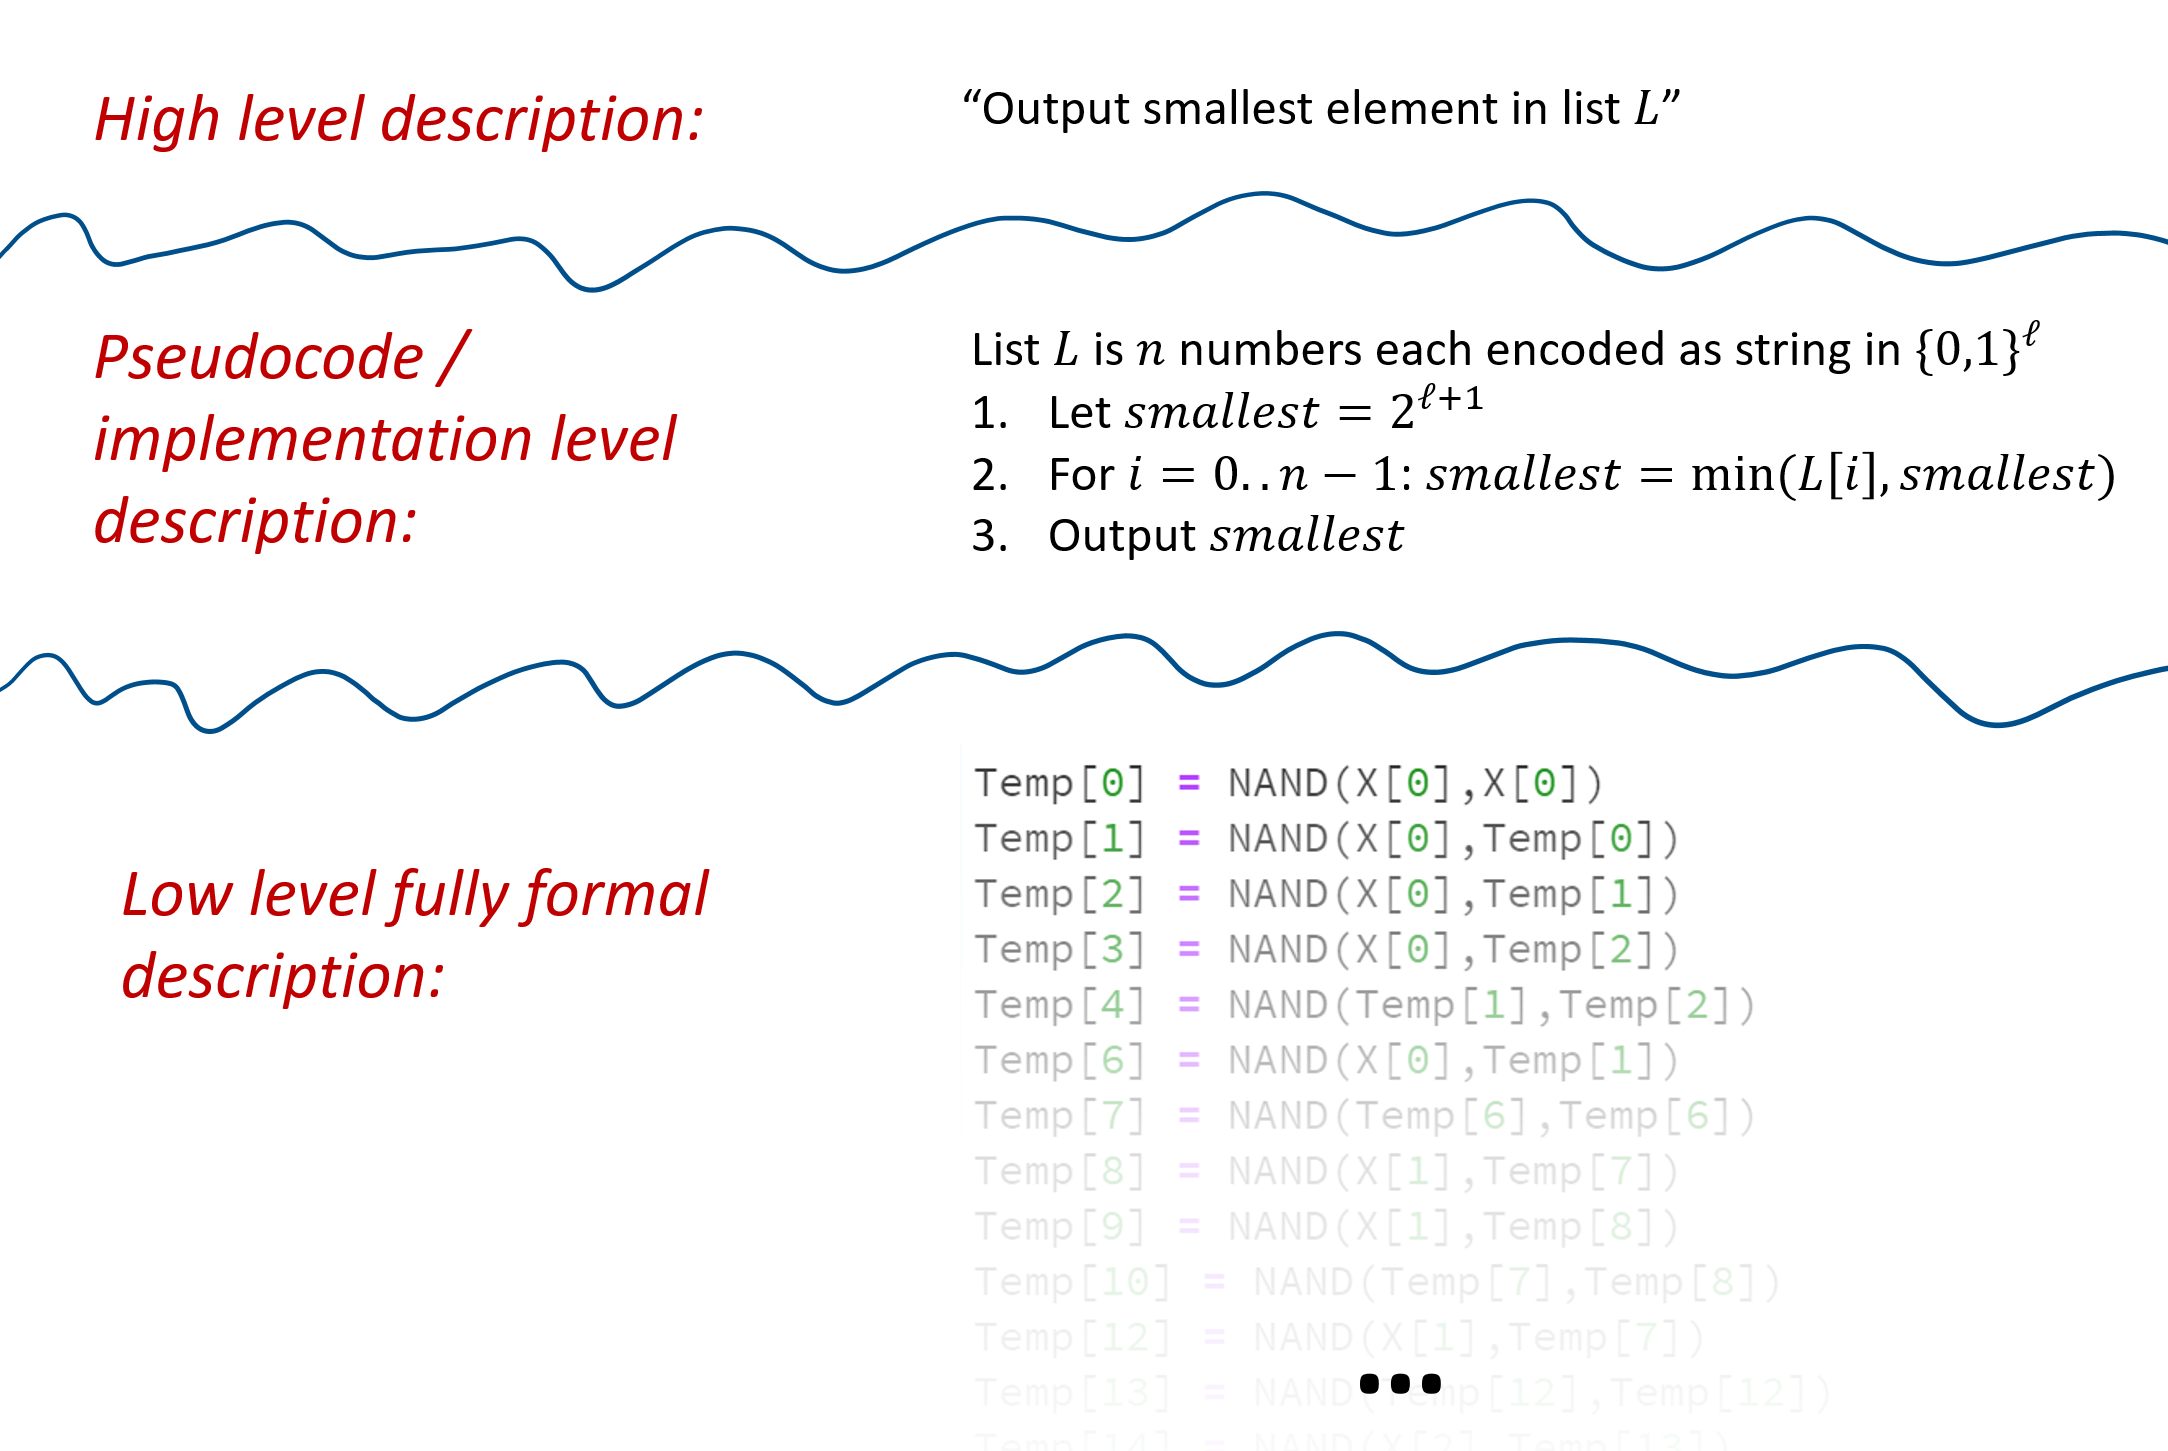
\includegraphics[width=\textwidth, height=0.25\paperheight, keepaspectratio]{../figure/levelsofdescription.png}
\caption{We can describe an algorithm at different levels of
granularity/detail and precision. At the highest level we just write the
idea in words, omitting all details on representation and
implementation. In the intermediate level (also known as
\emph{implementation} or \emph{pseudocode}) we give enough details of
the implementation that would allow someone to derive it, though we
still fall short of providing the full code. The lowest level is where
the actual code or mathematical description is fully spelled out. These
different levels of detail all have their uses, and moving between them
is one of the most important skills for a computer scientist.}
\label{levelsdescfig}
\end{figure}

While we started off by describing NAND-CIRC, NAND-TM, and NAND-RAM
programs at the full formal level, as we progress in this book we will
move to implementation and high level description. After all, our goal
is not to use these models for actual computation, but rather to analyze
the general phenomenon of computation. That said, if you don't
understand how the high level description translates to an actual
implementation, going ``down to the metal'' is often an excellent
exercise. One of the most important skills for a computer scientist is
the ability to move up and down hierarchies of abstractions.

A similar distinction applies to the notion of \emph{representation} of
objects as strings. Sometimes, to be precise, we give a \emph{low level
specification} of exactly how an object maps into a binary string. For
example, we might describe an encoding of \(n\) vertex graphs as length
\(n^2\) binary strings, by saying that we map a graph \(G\) over the
vertices \([n]\) to a string \(x\in \{0,1\}^{n^2}\) such that the
\(n\cdot i + j\)-th coordinate of \(x\) is \(1\) if and only if the edge
\(\overrightarrow{i \; j}\) is present in \(G\). We can also use an
\emph{intermediate} or \emph{implementation level} description, by
simply saying that we represent a graph using the adjacency matrix
representation.

Finally, because we are translating between the various representations
of graphs (and objects in general) can be done via a NAND-RAM (and hence
a NAND-TM) program, when talking in a high level we also suppress
discussion of representation altogether. For example, the fact that
graph connectivity is a computable function is true regardless of
whether we represent graphs as adjacency lists, adjacency matrices, list
of edge-pairs, and so on and so forth. Hence, in cases where the precise
representation doesn't make a difference, we would often talk about our
algorithms as taking as input an object \(X\) (that can be a graph, a
vector, a program, etc.) without specifying how \(X\) is encoded as a
string.

\paragraph{Defining Algorithms.} Up until now we have used the term
``algorithm'' informally. However, Turing Machines and the range of
equivalent models yield a way to precisely and formally define
algorithms. Hence whenever we refer to an \emph{algorithm} in this book,
we will mean that it is an instance of one of the Turing equivalent
models, such as Turing machines, NAND-TM, RAM machines, etc. Because of
the equivalence of all these models, in many contexts, it will not
matter which of these we use.

\subsection{Turing completeness and equivalence, a formal definition
(optional)}\label{turingcompletesec}

A \emph{computational model} is some way to define what it means for a
\emph{program} (which is represented by a string) to compute a (partial)
\emph{function}. A \emph{computational model} \(\mathcal{M}\) is
\emph{Turing complete}, if we can map every Turing machine (or
equivalently NAND-TM program) \(N\) into a program \(P\) for
\(\mathcal{M}\) that computes the same function as \(Q\). It is
\emph{Turing equivalent} if the other direction holds as well (i.e., we
can map every program in \(\mathcal{M}\) to a Turing machine that
computes the same function). We can define this notion formally as
follows. (This formal definition is not crucial for the remainder of
this book so feel to skip it as long as you understand the general
concept of Turing equivalence; This notion is sometimes referred to in
the literature as \href{https://goo.gl/rzuNPu}{Gödel numbering} or
\href{https://goo.gl/xXJoUG}{admissible numbering}.)

\hypertarget{turingcompletedef}{}
\begin{definition}[Turing completeness and equivalence (optional)] \label[definition]{turingcompletedef}

Let \(\mathcal{F}\) be the set of all partial functions from
\(\{0,1\}^*\) to \(\{0,1\}^*\). A \emph{computational model} is a map
\(\mathcal{M}:\{0,1\}^* \rightarrow \mathcal{F}\).

We say that a program \(P \in \{0,1\}^*\)
\emph{\(\mathcal{M}\)-computes} a function \(F\in \mathcal{F}\) if
\(\mathcal{M}(P) = F\).

A computational model \(\mathcal{M}\) is \emph{Turing complete} if there
is a computable map
\(\ensuremath{\mathit{ENCODE}}_{\mathcal{M}}:\{0,1\}^* \rightarrow \{0,1\}^*\)
for every Turing machine \(N\) (represented as a string),
\(\mathcal{M}(\ensuremath{\mathit{ENCODE}}_{\mathcal{M}}(N))\) is equal
to the partial function computed by \(N\).

A computational model \(\mathcal{M}\) is \emph{Turing equivalent} if it
is Turing complete and there exists a computable map
\(\ensuremath{\mathit{DECODE}}_{\mathcal{M}}:\{0,1\}^* \rightarrow \{0,1\}^*\)
such that or every string \(P\in \{0,1\}^*\),
\(N=\ensuremath{\mathit{DECODE}}_{\mathcal{M}}(P)\) is a string
representation of a Turing machine that computes the function
\(\mathcal{M}(P)\).

\end{definition}

Some examples of Turing equivalent models (some of which we have already
seen, and some are discussed below) include:

\begin{itemize}
\tightlist
\item
  Turing machines
\item
  NAND-TM programs
\item
  NAND-RAM programs
\item
  λ calculus
\item
  Game of life (mapping programs and inputs/outputs to starting and
  ending configurations)
\item
  Programming languages such as Python/C/Javascript/OCaml\ldots{}
  (allowing for unbounded storage)
\end{itemize}

\section{Cellular automata}\label{cellularautomatasec}

Many physical systems can be described as consisting of a large number
of elementary components that interact with one another. One way to
model such systems is using \emph{cellular automata}. This is a system
that consists of a large (or even infinite) number of cells. Each cell
only has a constant number of possible states. At each time step, a cell
updates to a new state by applying some simple rule to the state of
itself and its neighbors.


\begin{figure}
\centering
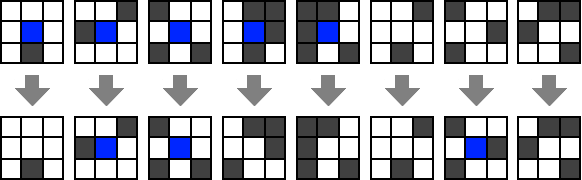
\includegraphics[width=\textwidth, height=0.25\paperheight, keepaspectratio]{../figure/conwaysgrids.png}
\caption{Rules for Conway's Game of Life. Image from
\href{https://mblogscode.wordpress.com/2017/06/07/python-simulation-coding-conways-game-of-life/}{this
blog post}.}
\label{gameofliferulesfig}
\end{figure}

A canonical example of a cellular automaton is
\href{https://en.wikipedia.org/wiki/Conway\%27s_Game_of_Life}{Conway's
Game of Life}. In this automata the cells are arranged in an infinite
two dimensional grid. Each cell has only two states: ``dead'' (which we
can encode as \(0\) and identify with \(\varnothing\)) or ``alive''
(which we can encode as \(1\)). The next state of a cell depends on its
previous state and the states of its 8 vertical, horizontal and diagonal
neighbors (see \cref{gameofliferulesfig}). A dead cell becomes alive
only if exactly three of its neighbors are alive. A live cell continues
to live if it has two or three live neighbors. Even though the number of
cells is potentially infinite, we can encode the state using a
finite-length string by only keeping track of the live cells. If we
initialize the system in a configuration with a finite number of live
cells, then the number of live cells will stay finite in all future
steps. The
\href{https://en.wikipedia.org/wiki/Conway\%27s_Game_of_Life}{Wikipedia
page} for the Game of Life contains some beautiful figures and
animations of configurations that produce very interesting evolutions.


\begin{figure}
\centering
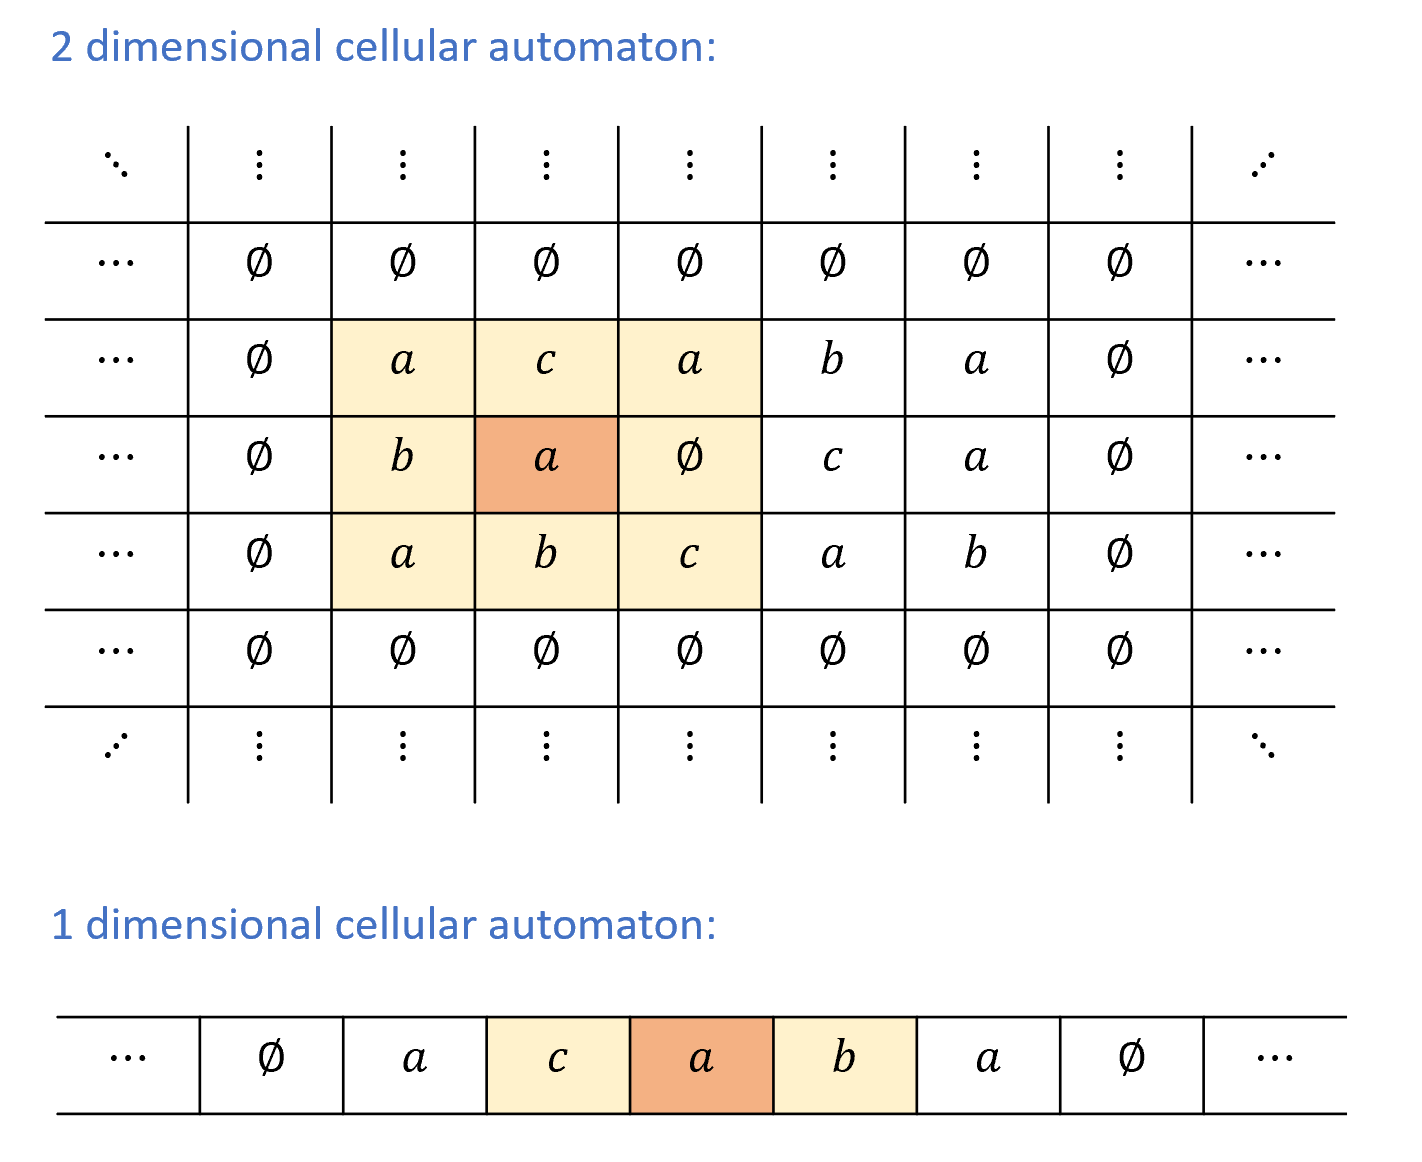
\includegraphics[width=\textwidth, height=0.25\paperheight, keepaspectratio]{../figure/onetwodimensionalca.png}
\caption{In a \emph{two dimensional cellular automaton} every cell is in
position \(i,j\) for some integers \(i,j \in \Z\). The \emph{state} of a
cell is some value \(A_{i,j} \in \Sigma\) for some finite alphabet
\(\Sigma\). At a given time step, the state of the cell is adjusted
according to some function applied to the state of \((i,j)\) and all its
neighbors \((i \pm 1, j\pm 1)\). In a \emph{one dimensional cellular
automaton} every cell is in position \(i\in \Z\) and the state \(A_i\)
of \(i\) at the next time step depends on its current state and the
state of its two neighbors \(i-1\) and \(i+1\).}
\label{onetwodimcellularautomatafig}
\end{figure}

Since the cells in the game of life are are arranged in an infinite
two-dimensional grid, it is an example of a \emph{two dimensional
cellular automaton}. We can also consider the even simpler setting of a
\emph{one dimensional cellular automaton}, where the cells are arranged
in an infinite line, see \cref{onetwodimcellularautomatafig}. It turns
out that even this simple model is enough to achieve
Turing-completeness. We will now formally define one-dimensional
cellular automata and then prove their Turing completeness.

\hypertarget{cellautomatadef}{}
\begin{definition}[One dimensional cellular automata] \label[definition]{cellautomatadef}

Let \(\Sigma\) be a finite set containing the symbol \(\varnothing\). A
\emph{one dimensional cellular automation} over alphabet \(\Sigma\) is
described by a \emph{transition rule} \(r:\Sigma^3 \rightarrow \Sigma\),
which satisfies
\(r(\varnothing,\varnothing,\varnothing) = \varnothing\).

A \emph{configuration} of the automaton \(r\) is a function
\(A:\Z \rightarrow \Sigma\). If an automaton with rule \(r\) is in
configuration \(A\), then its next configuration, denoted by
\(A' = \ensuremath{\mathit{NEXT}}_r(A)\), is the function \(A'\) such
that \(A'(i) = r(A(i-1),A(i),A(i+1))\) for every \(i\in \Z\). In other
words, the next state of the automaton \(r\) at point \(i\) obtained by
applying the rule \(r\) to the values of \(A\) at \(i\) and its two
neighbors.

\end{definition}

\paragraph{Finite configuration.} We say that a configuration of an
automaton \(r\) is \emph{finite} if there is only some finite number of
indices \(i_0,\ldots,i_{j-1}\) in \(\Z\) such that
\(A(i_j) \neq \varnothing\). (That is, for every
\(i \not\in \{ i_0, \ldots, i_{j-1}\}\), \(A(i)=\varnothing\).) Such a
configuration can be represented using a finite string that encodes the
indices \(i_0,\ldots,i_{n-1}\) and the values
\(A(i_0),\ldots,A(i_{n-1})\). Since
\(R(\varnothing,\varnothing,\varnothing)=\varnothing\), if \(A\) is a
finite configuration then \(\ensuremath{\mathit{NEXT}}_r(A)\) is finite
as well. We will only be interested in studying cellular automata that
are initialized in finite configurations, and hence remain in a finite
configuration throughout their evolution.

\subsection{One dimensional cellular automata are Turing
complete}\label{One-dimensional-cellular-}

We can write a program (for example using NAND-RAM) that simulates the
evolution of any cellular automaton from an initial finite configuration
by simply storing the values of the cells with state not equal to
\(\varnothing\) and repeatedly applying the rule \(r\). Hence cellular
automata can be simulated by Turing Machines. What is more surprising
that the other direction holds as well. For example, as simple as its
rules seem, we can simulate a Turing machine using the game of life (see
\cref{golfig}).


\begin{marginfigure}
\centering
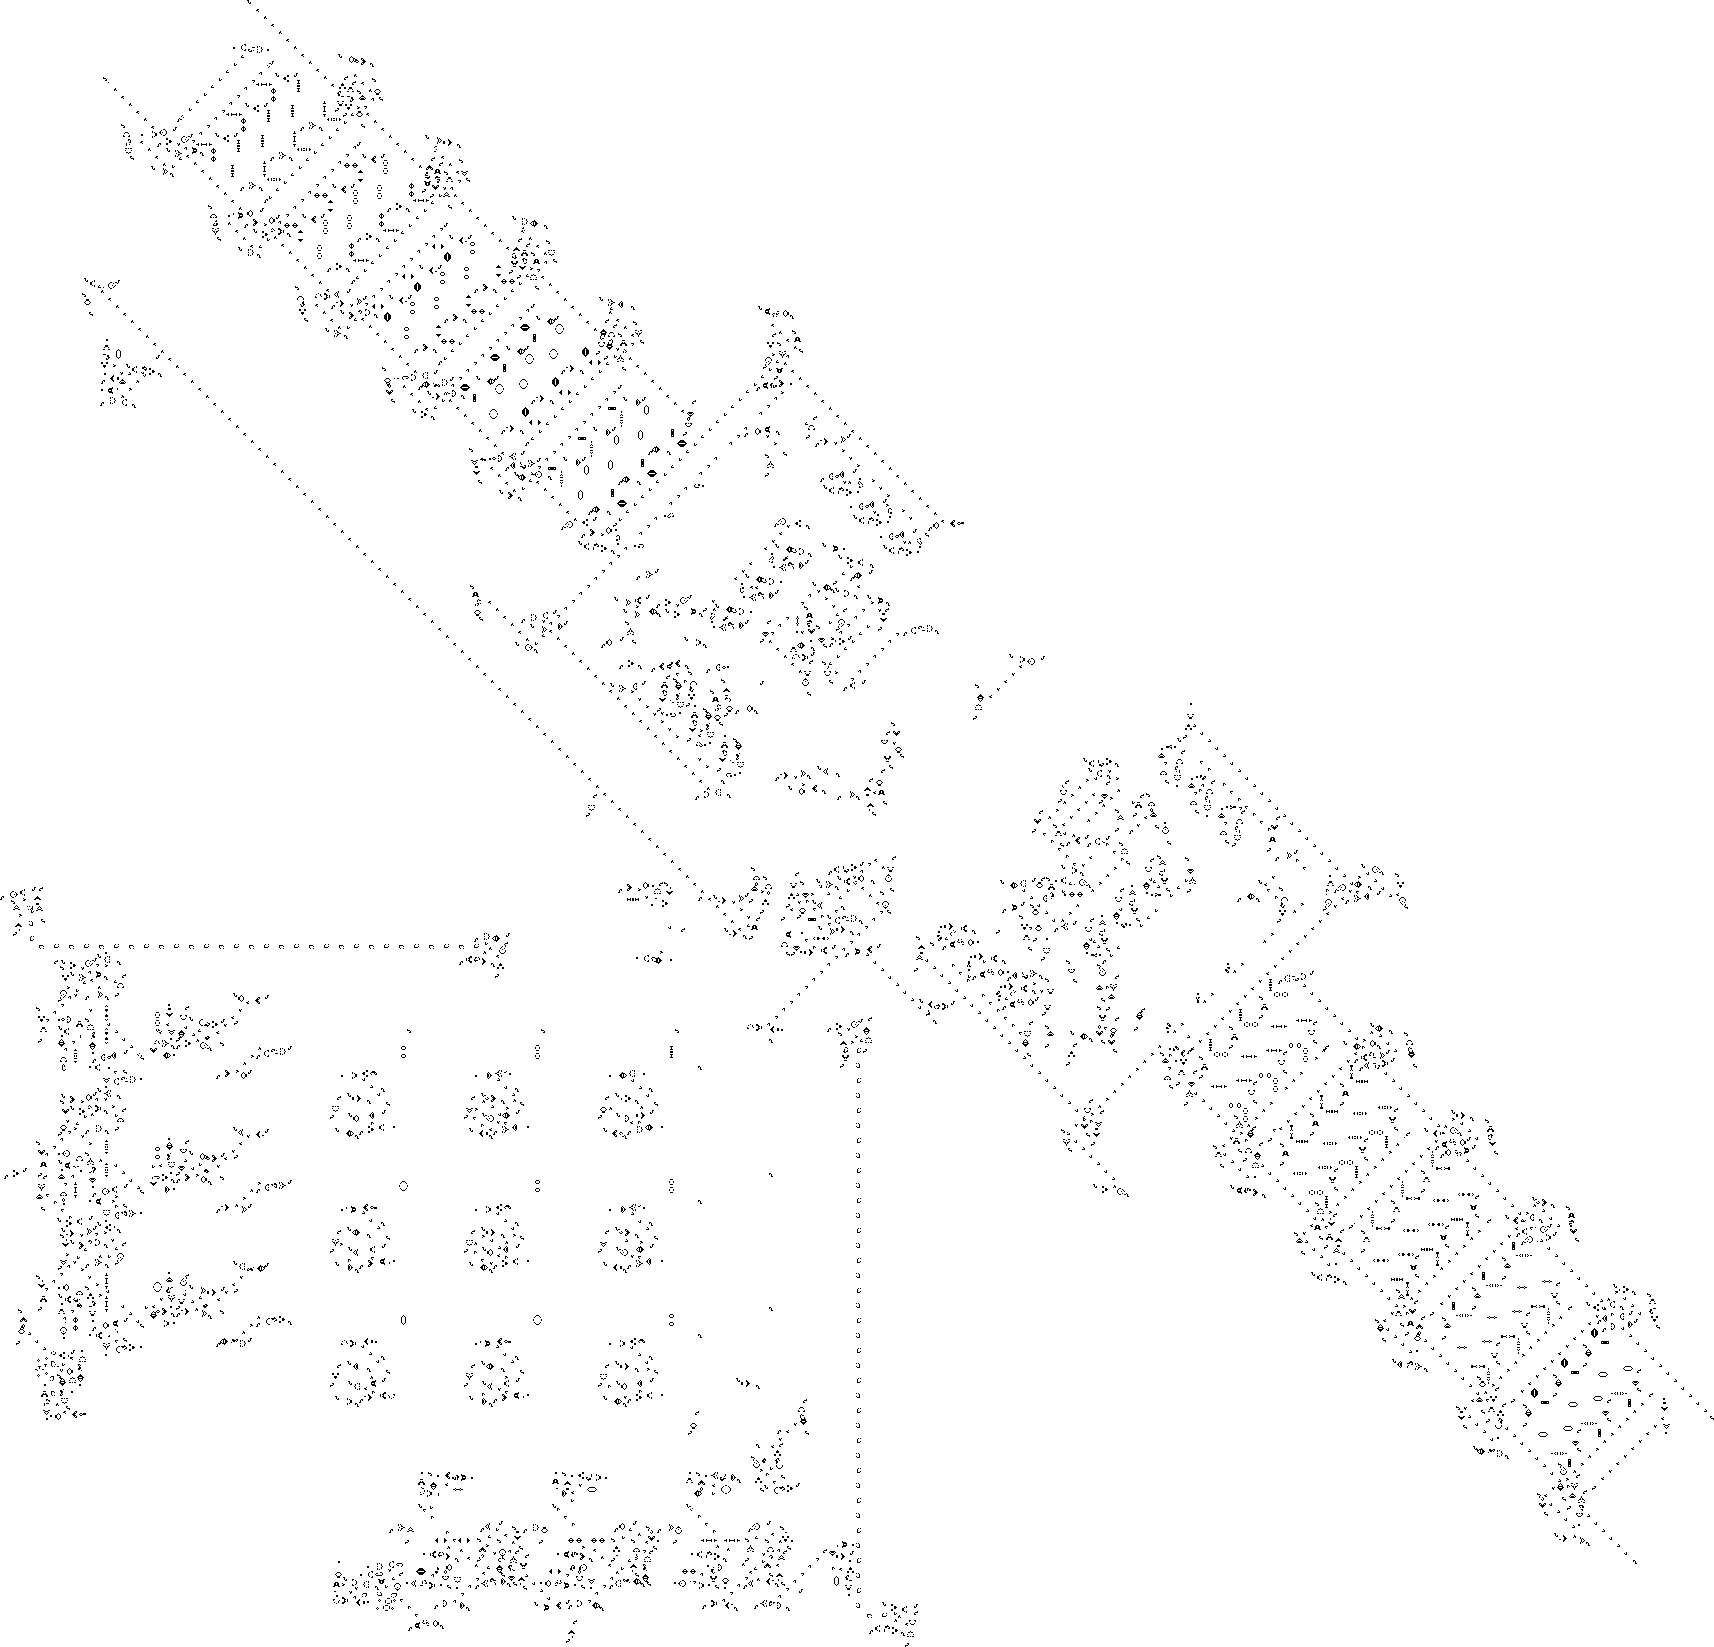
\includegraphics[width=\linewidth, height=1.5in, keepaspectratio]{../figure/turing_gol.jpg}
\caption{A Game-of-Life configuration simulating a Turing Machine.
Figure by \href{http://rendell-attic.org/gol/tm.htm}{Paul Rendell}.}
\label{golfig}
\end{marginfigure}

In fact, even \href{https://en.wikipedia.org/wiki/Rule_110}{one
dimensional cellular automata} can be Turing complete:

\hypertarget{onedimcathm}{}
\begin{theorem}[One dimensional automata are Turing complete] \label[theorem]{onedimcathm}

For every Turing machine \(M\), there is a one dimension cellular
automaton that can simulate \(M\) on every input \(x\).

\end{theorem}

To make the notion of ``simulating a Turing machine'' more precise we
will need to define \emph{configurations} of Turing machines. We will do
so in \cref{turingmachinesconfigsec} below, but at a high level a
\emph{configuration} of a Turing machine is a string that encodes its
full state at a given step in its computation. That is, the contents of
all (non empty) cells of its tape, its current state, as well as the
head position.

The key idea in the proof of \cref{onedimcathm} is that at every point
in the computation of a Turing machine \(M\), the only cell in \(M\)'s
tape that can change is the one where the head is located, and the value
this cell changes to is a function of its current state and the finite
state of \(M\). This observation allows us to encode the configuration
of a Turing machine \(M\) as a finite configuration of a cellular
automaton \(r\), and ensure that a one-step evolution of this encoded
configuration under the rules of \(r\) corresponds to one step in the
execution of the Turing machine \(M\).

\subsection{Configurations of Turing machines and the next-step
function}\label{turingmachinesconfigsec}

To turn the above ideas into a rigorous proof (and even statement!) of
\cref{onedimcathm} we will need to precisely define the notion of
\emph{configurations} of Turing machines. This notion will be useful for
us in later chapters as well.


\begin{figure}
\centering
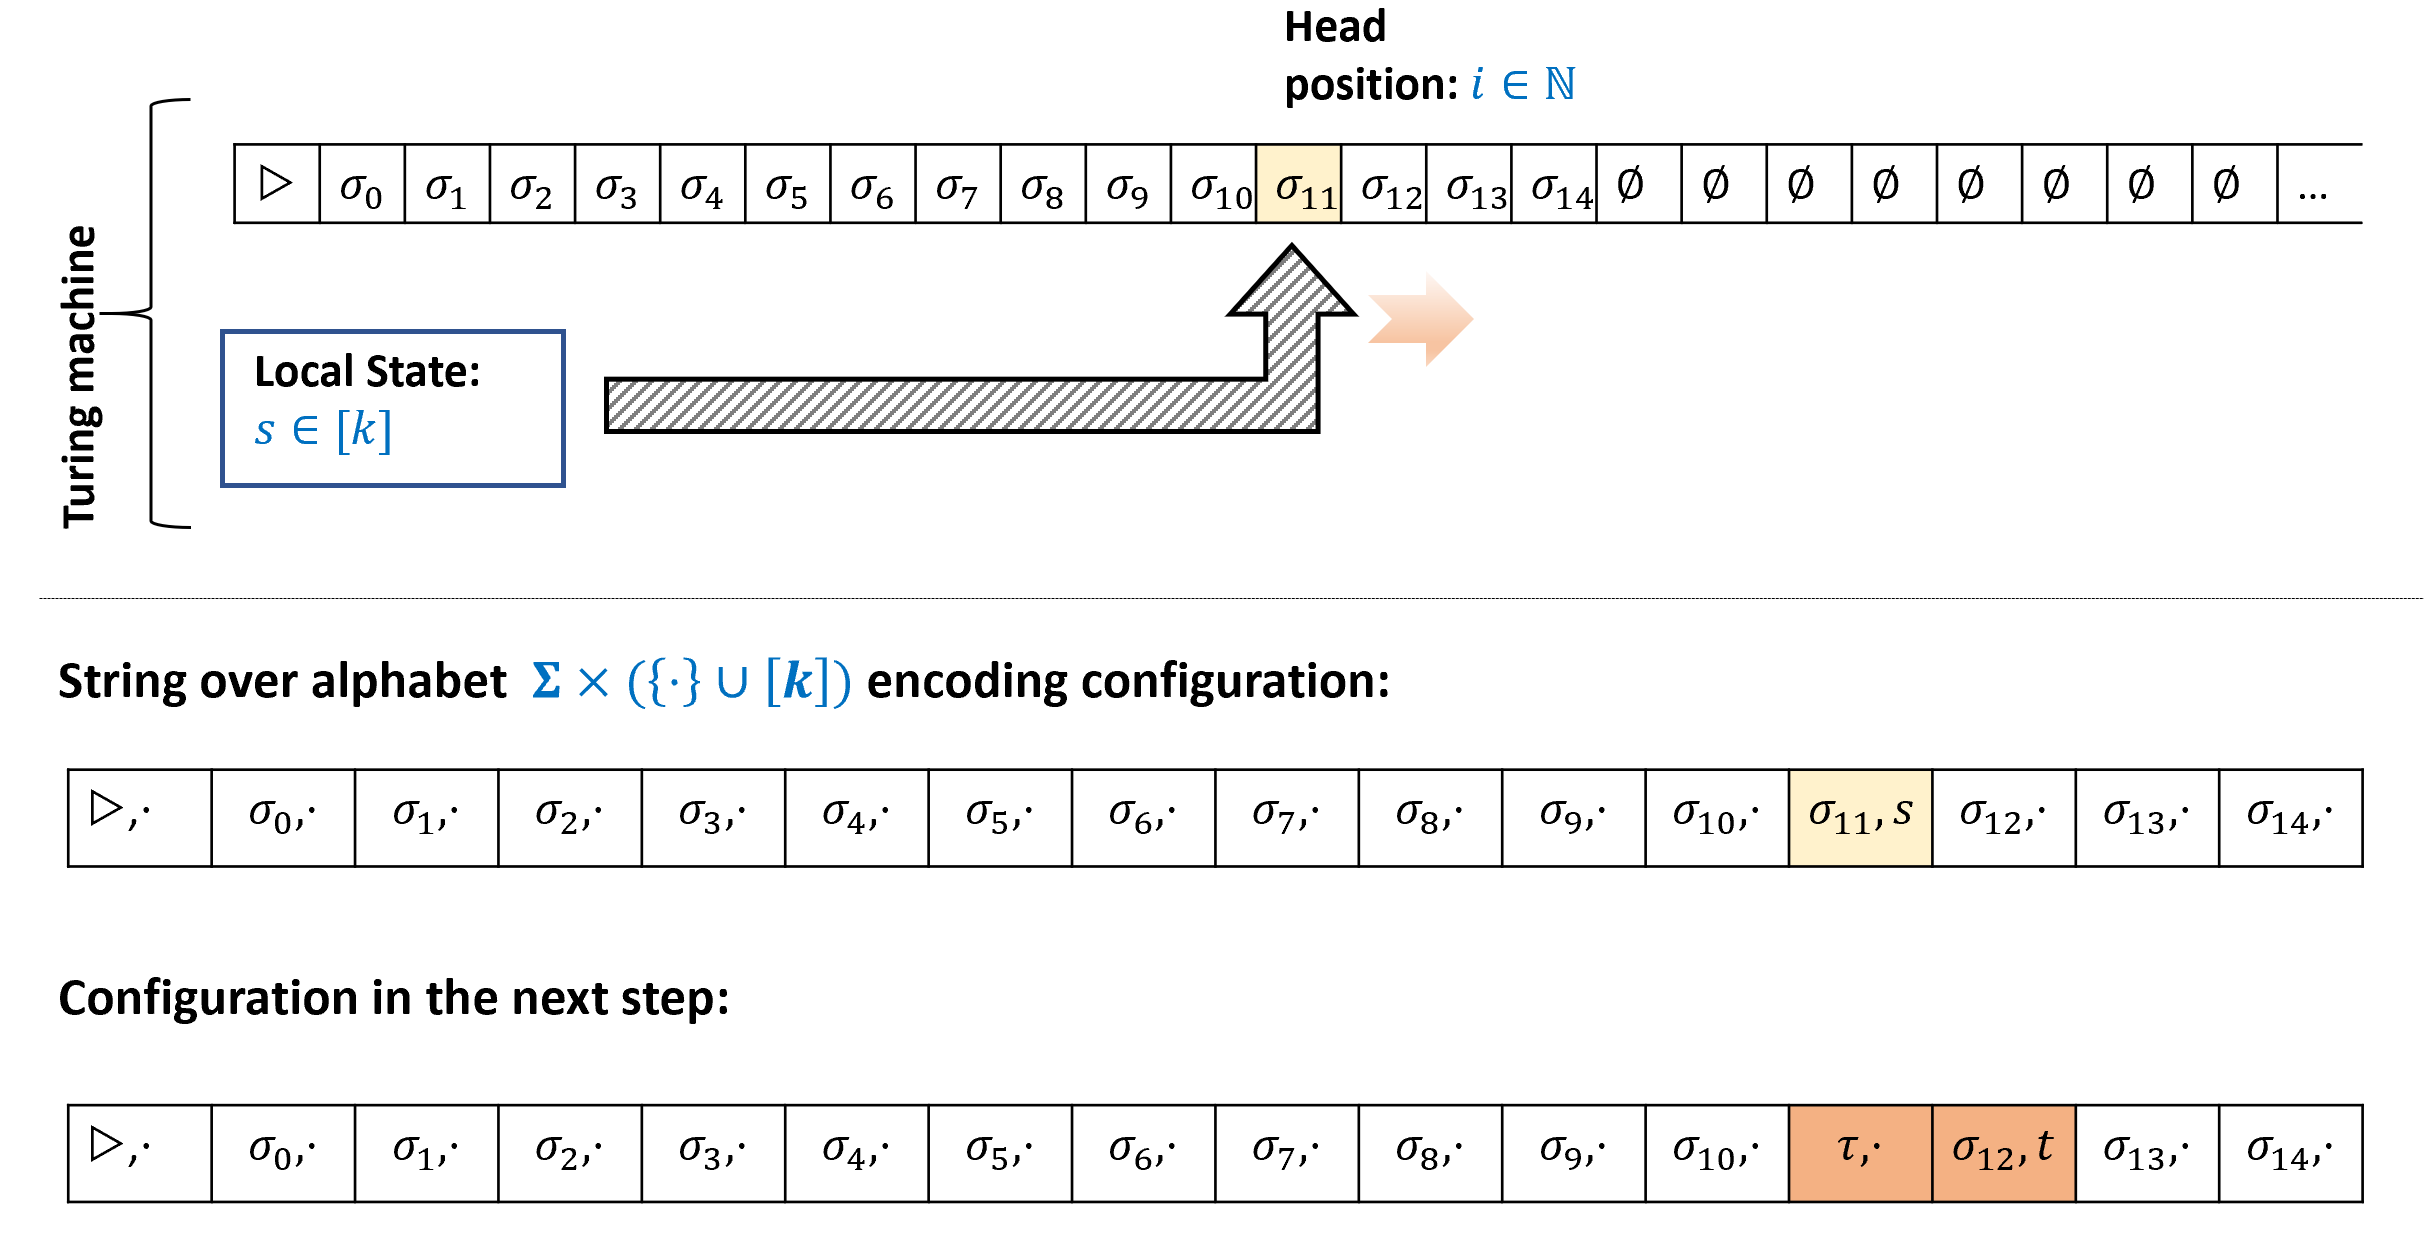
\includegraphics[width=\textwidth, height=0.25\paperheight, keepaspectratio]{../figure/turingmachineconf.png}
\caption{A \emph{configuration} of a Turing machine \(M\) with alphabet
\(\Sigma\) and state space \([k]\) encodes the state of \(M\) at a
particular step in its execution as a string \(\alpha\) over the
alphabet \(\overline{\Sigma} = \Sigma \times (\{\cdot \} \times [k])\).
The string is of length \(t\) where \(t\) is such that \(M\)'s tape
contains \(\varnothing\) in all positions \(t\) and larger and \(M\)'s
head is in a position smaller than \(t\). If \(M\)'s head is in the
\(i\)-th position, then for \(j \neq i\), \(\alpha_j\) encodes the value
of the \(j\)-th cell of \(M\)'s tape, while \(\alpha_i\) encodes both
this value as well as the current state of \(M\). If the machine writes
the value \(\tau\), changes state to \(t\), and moves right, then in the
next configuration will contain at position \(i\) the value
\((\tau,\cdot)\) and at position \(i+1\) the value
\((\alpha_{i+1},t)\).}
\label{turingconfigfig}
\end{figure}

\hypertarget{configtmdef}{}
\begin{definition}[Configuration of Turing Machines.] \label[definition]{configtmdef}

Let \(M\) be a Turing machine with tape alphabet \(\Sigma\) and state
space \([k]\). A \emph{configuration of \(M\)} is a string
\(\alpha \in \overline{\Sigma}^*\) where
\(\overline{\Sigma} = \Sigma \times \left( \{\cdot\} \cup [k] \right)\)
that satisfies that there is exactly one coordinate \(i\) for which
\(\alpha_i = (\sigma,s)\) for some \(\sigma \in \Sigma\) and
\(s\in [k]\). For all other coordinates \(j\),
\(\alpha_j = (\sigma',\cdot)\) for some \(\sigma'\in \Sigma\).

A configuration \(\alpha \in \overline{\Sigma}^*\) of \(M\) corresponds
to the following state of its execution:

\begin{itemize}
\item
  \(M\)'s tape contains \(\alpha_{j,0}\) for all \(j<|\alpha|\) and
  contains \(\varnothing\) for all positions that are at least
  \(|\alpha|\), where we let \(\alpha_{j,0}\) be the value \(\sigma\)
  such that \(\alpha_j = (\sigma,t)\) with \(\sigma \in \Sigma\) and
  \(t \in \{\cdot \} \cup [k]\). (In other words, since \(\alpha_j\) is
  a pair of an alphabet symbol \(\sigma\) and either a state in \([k]\)
  or the symbol \(\cdot\), \(\alpha_{j,0}\) is the first component
  \(\sigma\) of this pair.)
\item
  \(M\)'s head is in the unique position \(i\) for which \(\alpha_i\)
  has the form \((\sigma,s)\) for \(s\in [k]\), and \(M\)'s state is
  equal to \(s\).
\end{itemize}

\end{definition}

\begin{pause} \label[pause]{crefconfigtmdef-below-has}

\cref{configtmdef} below has some technical details, but is not actually
that deep or complicated. Try to take a moment to stop and think how
\emph{you} would encode as a string the state of a Turing machine at a
given point in an execution.

Think what are all the components that you need to know in order to be
able to continue the execution from this point onwards, and what is a
simple way to encode them using a list of finite symbols. In particular,
with an eye towards our future applications, try to think of an encoding
which will make it as simple as possible to map a configuration at step
\(t\) to the configuration at step \(t+1\).

\end{pause}

\cref{configtmdef} is a little cumbersome, but ultimately a
configuration is simply a string that encodes a \emph{snapshot} of the
Turing machine at a given point in the execution. (In operating-systems
lingo, it is a \href{https://goo.gl/AsccXh}{``core dump''}.) Such a
snapshot needs to encode the following components:

\begin{enumerate}
\def\labelenumi{\arabic{enumi}.}
\item
  The current head position.
\item
  The full contents of the large scale memory, that is the tape.
\item
  The contents of the ``local registers'', that is the state of the
  machine.
\end{enumerate}

The precise details of how we encode a configuration are not important,
but we do want to record the following simple fact:

\hypertarget{nextstepfunctionlem}{}
\begin{lemma} \label[lemma]{nextstepfunctionlem}

Let \(M\) be a Turing machine and let
\(\ensuremath{\mathit{NEXT}}_M:\overline{\Sigma}^* \rightarrow \overline{\Sigma}^*\)
be the function that maps a configuration of \(M\) to the configuration
at the next step of the execution. Then for every \(i \in \N\), the
value of \(\ensuremath{\mathit{NEXT}}_M(\alpha)_i\) only depends on the
coordinates \(\alpha_{i-1},\alpha_i,\alpha_{i+1}\).

\end{lemma}

(For simplicity of notation, above we use the convention that if \(i\)
is ``out of bounds'', such as \(i<0\) or \(i>|\alpha|\), then we assume
that \(\alpha_i = (\varnothing,\cdot)\).) We leave proving
\cref{nextstepfunctionlem} as \cref{nextstepfunctionlemex}. The idea
behind the proof is simple: if the head is neither in position \(i\) nor
positions \(i-1\) and \(i+1\), then the next-step configuration at \(i\)
will be the same as it was before. Otherwise, we can ``read off'' the
state of the Turing machine and the value of the tape at the head
location from the configuration at \(i\) or one of its neighbors and use
that to update what the new state at \(i\) should be. Completing the
full proof is not hard, but doing it is a great way to ensure that you
are comfortable with the definition of configurations.

\paragraph{Completing the proof of \cref{onedimcathm}.} We can now
restate \cref{onedimcathm} more formally, and complete its proof:

\hypertarget{onedimcathmformal}{}
\begin{theorem}[One dimensional automata are Turing complete (formal statement)] \label[theorem]{onedimcathmformal}

For every Turing Machine \(M\), if we denote by \(\overline{\Sigma}\)
the alphabet of its configuration strings, then there is a
one-dimensional cellular automaton \(r\) over the alphabet
\(\overline{\Sigma}^*\) such that
\[\left( \ensuremath{\mathit{NEXT}}_M(\alpha) \right)  = \ensuremath{\mathit{NEXT}}_r \left( \alpha \right)\]
for every configuration \(\alpha \in \overline{\Sigma}^*\) of \(M\)
(again using the convention that we consider \(\alpha_i=\varnothing\) if
\(i\) is "out of bounds).

\end{theorem}

\begin{proof} \label[proof]{We-consider-the-element-v}

We consider the element \((\varnothing,\cdot)\) of \(\overline{\Sigma}\)
to correspond to the \(\varnothing\) element of the automaton \(r\). In
this case, by \cref{nextstepfunctionlem}, the function
\(\ensuremath{\mathit{NEXT}}_M\) that maps a configuration of \(M\) into
the next one is in fact a valid rule for a one dimensional automata.

\end{proof}

The automaton arising from the proof of \cref{onedimcathmformal} has a
large alphabet, and furthermore one whose size that depends on the
machine \(M\) that is being simulated. It turns out that one can obtain
an automaton with an alphabet of fixed size that is independent of the
program being simulated, and in fact the alphabet of the automaton can
be the minimal set \(\{0,1\}\)! See \cref{onedimautfig} for an example
of such an Turing-complete automaton.


\begin{marginfigure}
\centering
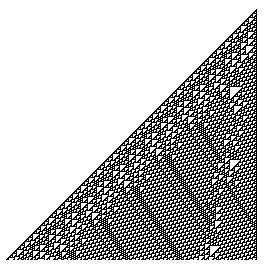
\includegraphics[width=\linewidth, height=1.5in, keepaspectratio]{../figure/Rule110Big.jpg}
\caption{Evolution of a one dimensional automata. Each row in the figure
corresponds to the configuration. The initial configuration corresponds
to the top row and contains only a single ``live'' cell. This figure
corresponds to the ``Rule 110'' automaton of Stephen Wolfram which is
Turing Complete. Figure taken from
\href{http://mathworld.wolfram.com/Rule110.html}{Wolfram MathWorld}.}
\label{onedimautfig}
\end{marginfigure}

\hypertarget{nandtmprogconfig}{}
\begin{remark}[Configurations of NAND-TM programs] \label[remark]{nandtmprogconfig}

We can use the same approach as \cref{configtmdef} to define
configurations of a \emph{NAND-TM program}. Such a configuration will
need to encode:

\begin{enumerate}
\def\labelenumi{\arabic{enumi}.}
\item
  The current value of the variable \texttt{i}.
\item
  For every scalar variable \texttt{foo}, the value of \texttt{foo}.
\item
  For every array variable \texttt{Bar}, the value
  \texttt{Bar[}\(j\)\texttt{]} for every \(j \in \{0,\ldots, t-1\}\)
  where \(t-1\) is the largest value that the index variable \texttt{i}
  ever achieved in the computation.
\end{enumerate}

\end{remark}

\section{Lambda calculus and functional programming
languages}\label{lambdacalculussec}

The \href{https://goo.gl/B9HwT8}{λ calculus} is another way to define
computable functions. It was proposed by Alonzo Church in the 1930's
around the same time as Alan Turing's proposal of the Turing Machine.
Interestingly, while Turing Machines are not used for practical
computation, the λ calculus has inspired functional programming
languages such as LISP, ML and Haskell, and indirectly the development
of many other programming languages as well. In this section we will
present the λ calculus and show that its power is equivalent to NAND-TM
programs (and hence also to Turing machines). Our
\href{https://github.com/boazbk/tcscode}{Github repository} contains a
Jupyter notebook with a Python implementation of the λ calculus that you
can experiment with to get a better feel for this topic.

\paragraph{The λ operator.} At the core of the λ calculus is a way to
define ``anonymous'' functions. For example, instead of giving a name
\(f\) to a function and defining it as

\[
f(x) = x\times x
\]

we can write it as

\[
\lambda x. x\times x
\]

and so \((\lambda x.x\times x)(7)=49\). That is, you can think of
\(\lambda x. exp(x)\), where \(exp\) is some expression as a way of
specifying the anonymous function \(x \mapsto exp(x)\). Anonymous
functions, using either \(\lambda x.f(x)\), \(x \mapsto f(x)\) or other
closely related notation, appear in many programming languages. For
example, in \emph{Python} we can define the squaring function using
\texttt{lambda x: x*x} while in \emph{JavaScript} we can use
\texttt{x => x*x} or \texttt{(x) => x*x}. In \emph{Scheme} we would
define it as \texttt{(lambda (x) (* x x))}. Clearly, the name of the
argument to a function doesn't matter, and so \(\lambda y.y\times y\) is
the same as \(\lambda x.x \times x\), as both correspond to the squaring
function.

\emph{Dropping parenthesis.} To reduce notational clutter, when writing
\(\lambda\) calculus expressions we often drop the parentheses for
function evaluation. Hence instead of writing \(f(x)\) for the result of
applying the function \(f\) to the input \(x\), we can also write this
as simply \(f\; x\). Therefore we can write
\((\lambda x.x\times x) 7=49\). In this chapter, we will use both the
\(f(x)\) and \(f\; x\) notations for function application. Function
evaluations are associative and bind from left to right, and hence
\(f\;g\;h\) is the same as \((f g) h\).

\subsection{Applying functions to
functions}\label{Applying-functions-to-fun}

A key feature of the λ calculus is that functions are ``first-class
objects'' in the sense that we can use functions as arguments to other
functions. For example, can you guess what number is the following
expression equal to?

\[(((\lambda f.(\lambda y.(f \;(f\; y)))) (\lambda x. x\times x))\; 3) \label{lambdaexampleeq}\]

\begin{pause} \label[pause]{The-expression-eqreflambd}

The expression \eqref{lambdaexampleeq} might seem daunting, but before
you look at the solution below, try to break it apart to its components,
and evaluate each component at a time. Working out this example would go
a long way toward understanding the λ calculus.

\end{pause}

Let's evaluate \eqref{lambdaexampleeq} one step at a time. As nice as it
is for the λ calculus to allow anonymous functions, adding names can be
very helpful for understanding complicated expressions. So, let us write
\(F = \lambda f.(\lambda y.(f (f y)))\) and \(g = \lambda x.x\times x\).

Therefore \eqref{lambdaexampleeq} becomes \[
((F \; g)\;  3) \;.
\]

On input a function \(f\), \(F\) outputs the function
\(\lambda y.(f (f\; y))\), or in other words \(F f\) is the function
\(y \mapsto f(f(y))\). Our function \(g\) is simply \(g(x)=x^2\) and so
\((F g)\) is the function that maps \(y\) to \((y^2)^2= y^4\). Hence
\(((F g) 3) = 3^4 = 81\).

\hypertarget{lambdaexptwoex}{}
\begin{solvedexercise} \label[solvedexercise]{lambdaexptwoex}

What number does the following expression equal to?

\[((\lambda x.(\lambda y.x)) \; 2)\; 9) \;. \label{lambdaexptwoeq}\]

\end{solvedexercise}

\begin{solution} \label[solution]{lambda-yx-is-the-function}

\(\lambda y.x\) is the function that on input \(y\) ignores its input
and outputs \(x\). Hence \((\lambda x.(\lambda y.x)) 2\) yields the
function \(y \mapsto 2\) (or, using \(\lambda\) notation, the function
\(\lambda y. 2\)). Hence \eqref{lambdaexptwoeq} is equivalent to
\((\lambda y. 2) 9 = 2\).

\end{solution}

\subsection{Obtaining multi-argument functions via
Currying}\label{curryingsec}

In a λ expression of the form \(\lambda x. e\), the expression \(e\) can
itself involve the λ operator. Thus for example the function

\[
\lambda x. (\lambda y. x+y) \label{eqlambdaexampleone}
\]

maps \(x\) to the function \(y \mapsto x+y\).

In particular, if we invoke the function \eqref{eqlambdaexampleone} on
\(a\) to obtain some function \(f\), and then invoke \(f\) on \(b\), we
obtain the value \(a+b\). We can see that the one-argument function
\eqref{eqlambdaexampleone} corresponding to
\(a \mapsto (b \mapsto a+b)\) can also be thought of as the two-argument
function \((a,b) \mapsto a+b\). Generally, we can use the λ expression
\(\lambda x.(\lambda y.f(x,y))\) to simulate the effect of a two
argument function \((x,y) \mapsto f(x,y)\). This technique is known as
\href{https://en.wikipedia.org/wiki/Currying}{Currying}. We will use the
shorthand \(\lambda x,y. e\) for \(\lambda x. (\lambda y. e)\). If
\(f= \lambda x.(\lambda y.e)\) then \((f a) b\) corresponds to applying
\(f a\) and then invoking the resulting function on \(b\), obtaining the
result of replacing in \(e\) the occurrences of \(x\) with \(a\) and
occurrences of \(b\) with \(y\). By our rules of associativity, this is
the same as \((f a b)\) which we'll sometimes also write as \(f(a,b)\).


\begin{marginfigure}
\centering
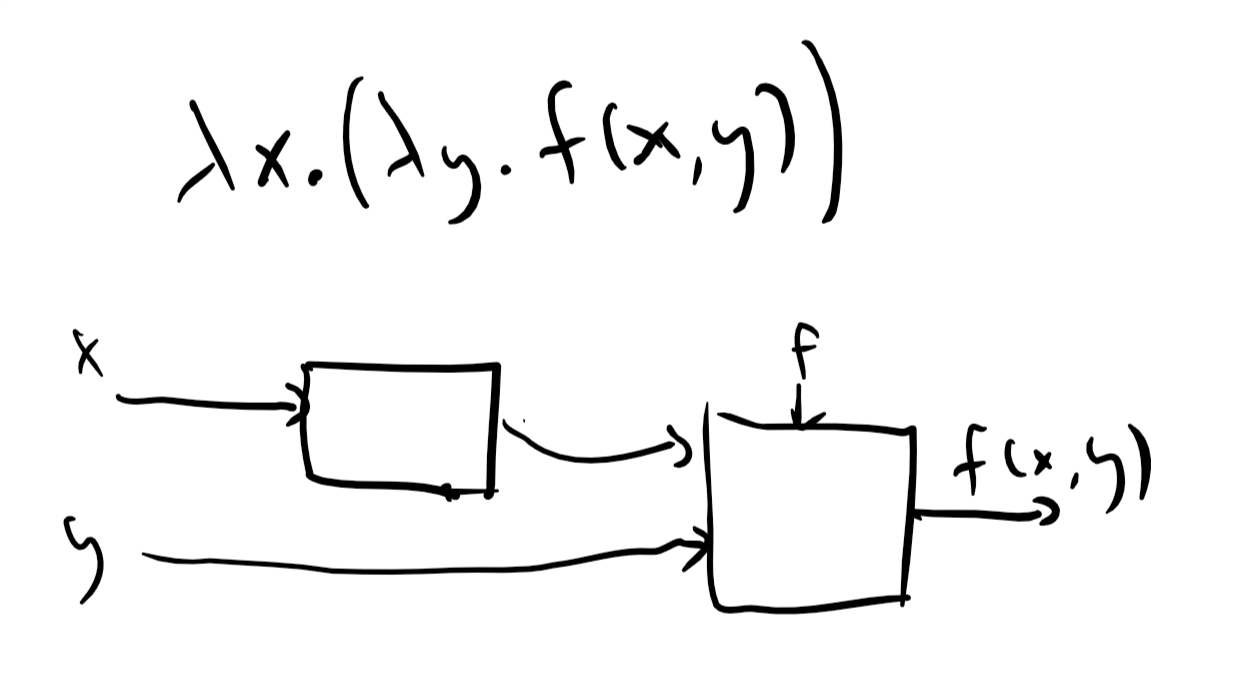
\includegraphics[width=\linewidth, height=1.5in, keepaspectratio]{../figure/currying.png}
\caption{In the ``currying'' transformation, we can create the effect of
a two parameter function \(f(x,y)\) with the λ expression
\(\lambda x.(\lambda y. f(x,y))\) which on input \(x\) outputs a
one-parameter function \(f_x\) that has \(x\) ``hardwired'' into it and
such that \(f_x(y)=f(x,y)\). This can be illustrated by a circuit
diagram; see \href{https://tromp.github.io/cl/diagrams.html}{Chelsea
Voss's site}.}
\label{currying}
\end{marginfigure}

\subsection{Formal description of the λ
calculus.}\label{Formal-description-of-the}

We now provide a formal description of the λ calculus. We start with
``basic expressions'' that contain a single variable such as \(x\) or
\(y\) and build more complex expressions of the form \((e \; e')\) and
\(\lambda x.e\) where \(e,e'\) are expressions and \(x\) is a variable
idenifier. Formally λ expressions are defined as follows:

\hypertarget{lambdaexpdef}{}
\begin{definition}[λ expression.] \label[definition]{lambdaexpdef}

A \emph{λ expression} is either a single variable identifier or an
expression \(e\) of the one of the following forms:

\begin{itemize}
\item
  \textbf{Application:} \(e = (e' \; e'')\), where \(e'\) and \(e''\)
  are λ expressions.
\item
  \textbf{Abstraction:} \(e = \lambda x.(e')\) where \(e'\) is a λ
  expression.
\end{itemize}

\end{definition}

\cref{lambdaexpdef} is a \emph{recursive definition} since we defined
the concept of λ expressions in terms of itself. This might seem
confusing at first, but in fact you have known recursive definitions
since you were an elementary school student. Consider how we define an
\emph{arithmetic expression}: it is an expression that is either just a
number, or has one of the forms \((e + e')\), \((e - e')\),
\((e \times e')\), or \((e \div e')\), where \(e\) and \(e'\) are other
arithmetic expressions.

\emph{Free and bound variables.} Variables in a λ expression can either
be \emph{free} or \emph{bound} to a \(\lambda\) operator (in the sense
of \cref{boundvarsec}). In a single-variable λ expression \(var\), the
variable \(var\) is free. The set of free and bound variables in an
application expression \(e = (e' \; e'')\) is the same as that of the
underlying expressions \(e'\) and \(e''\). In an abstraction expression
\(e = \lambda var.(e')\), all free occurences of \(var\) in \(e'\) are
bound to the \(\lambda\) operator of \(e\). If you find the notion of
free and bound variables confusing, you can avoid all these issues by
using unique identifiers for all variables.

\emph{Precedence and parenthesis.} We will use the following rules to
allow us to drop some parenthesis. Function application associates from
left to right, and so \(fgh\) is the same as \((fg)h\). Function
application has a higher precedence than the λ operator, and so
\(\lambda x.fgx\) is the same as \(\lambda x.((fg)x)\). This is similar
to how we use the precedence rules in arithmetic operations to allow us
to use fewer parenthesis and so write the expression
\((7 \times 3) + 2\) as \(7\times 3 + 2\). As mentioned in
\cref{curryingsec}, we also use the shorthand \(\lambda x,y.e\) for
\(\lambda x.(\lambda y.e)\) and the shorthand \(f(x,y)\) for
\((f\; x)\; y\). This plays nicely with the ``Currying'' transformation
of simulating multi-input functions using λ expressions.

\paragraph{Equivalence of λ expressions.} As we have seen in
\cref{lambdaexptwoex}, the rule that \((\lambda x. exp) exp'\) is
equivalent to \(exp[x \rightarrow exp']\) enables us to modify λ
expressions and obtain simpler \emph{equivalent form} for them. Another
rule that we can use is that the parameter does not matter and hence for
example \(\lambda y.y\) is the same as \(\lambda z.z\). Together these
rules define the notion of \emph{equivalence} of λ expressions:

\hypertarget{lambdaequivalence}{}
\begin{definition}[Equivalence of λ expressions] \label[definition]{lambdaequivalence}

Two λ expressions are \emph{equivalent} if they can be made into the
same expression by repeated applications of the following rules:

\begin{enumerate}
\def\labelenumi{\arabic{enumi}.}
\item
  \textbf{Evaluation (aka \(\beta\) reduction):} The expression
  \((\lambda x.exp) exp'\) is equivalent to \(exp[x \rightarrow exp']\).
\item
  \textbf{Variable renaming (aka \(\alpha\) conversion):} The expression
  \(\lambda x.exp\) is equivalent to \(\lambda y.exp[x \rightarrow y]\).
\end{enumerate}

\end{definition}

If \(exp\) is a λ expression of the form \(\lambda x.exp'\) then it
naturally corresponds to the function that maps any input \(z\) to
\(exp'[x \rightarrow z]\). Hence the λ calculus naturally implies a
computational model. Since in the λ calculus the inputs can themselves
be functions, we need to decide in what order we evaluate an expression
such as

\[
(\lambda x.f)(\lambda y.g z) \;. \label{lambdaexpeq}
\] There are two natural conventions for this:

\begin{itemize}
\item
  \emph{Call by name} (aka \emph{``lazy evaluation''}): We evaluate
  \eqref{lambdaexpeq} by first plugging in the righthand expression
  \((\lambda y.g z)\) as input to the lefthand side function, obtaining
  \(f[x \rightarrow (\lambda y.g z)]\) and then continue from there.
\item
  \emph{Call by value} (aka \emph{``eager evaluation''}): We evaluate
  \eqref{lambdaexpeq} by first evaluating the righthand side and
  obtaining \(h=g[y \rightarrow z]\), and then plugging this into the
  lefthandside to obtain \(f[x \rightarrow h]\).
\end{itemize}

Because the λ calculus has only \emph{pure} functions, that do not have
``side effects'', in many cases the order does not matter. In fact, it
can be shown that if we obtain a definite irreducible expression (for
example, a number) in both strategies, then it will be the same one.
However, for concreteness we will always use the ``call by name'' (i.e.,
lazy evaluation) order. (The same choice is made in the programming
language Haskell, though many other programming languages use eager
evaluation.) Formally, the evaluation of a λ expression using ``call by
name'' is captured by the following process:

\hypertarget{simplifylambdadef}{}
\begin{definition}[Simplification of λ expressions] \label[definition]{simplifylambdadef}

Let \(e\) be a λ expression. The \emph{simplification} of \(e\) is the
result of the following recursive process:

\begin{enumerate}
\def\labelenumi{\arabic{enumi}.}
\item
  If \(e\) is a single variable \(x\) then the simplification of \(e\)
  is \(e\).
\item
  If \(e\) has the form \(e= \lambda x.e'\) then the simplification of
  \(e\) is \(\lambda x.f'\) where \(f'\) is the simplification of
  \(e'\).
\item
  \emph{(Evaluation / \(\beta\) reduction.)} If \(e\) has the form
  \(e=(\lambda x.e' \; e'')\) then the simplification of \(e\) is the
  simplification of \(e'[x \rightarrow e'']\), which denotes replacing
  all copies of \(x\) in \(e'\) bound to the \(\lambda\) operator with
  \(e''\)
\item
  \emph{(Renaming / \(\alpha\) conversion.)} The \emph{canonical
  simplification} of \(e\) is obtained by taking the simplification of
  \(e\) and renaming the variables so that the first bound variable in
  the expression is \(v_0\), the second one is \(v_1\), and so on and so
  forth.
\end{enumerate}

We say that two λ expressions \(e\) and \(e'\) are \emph{equivalent},
denoted by \(e \cong e'\), if they have the same canonical
simplification.

\end{definition}

\hypertarget{lambdaeuivexer}{}
\begin{solvedexercise}[Equivalence of λ expressions] \label[solvedexercise]{lambdaeuivexer}

Prove that the following two expressions \(e\) and \(f\) are equivalent:

\[e = \lambda x.x\]

\[f = (\lambda a.(\lambda b.b)) (\lambda z.zz)\]

\end{solvedexercise}

\begin{solution} \label[solution]{The-canonical-simplificat}

The canonical simplification of \(e\) is simply \(\lambda v_0.v_0\). To
do the canonical simplification of \(f\) we first use \(\beta\)
reduction to plug in \(\lambda z.zz\) instead of \(a\) in
\((\lambda b.b)\) but since \(a\) is not used in this function at all,
we simply obtained \(\lambda b.b\) which simplifies to
\(\lambda v_0.v_0\) as well.

\end{solution}

\subsection{Infinite loops in the λ calculus}\label{infiniteloopslambda}

Like Turing machines and NAND-TM programs, the simplification process in
the λ calculus can also enter into an infinite loop. For example,
consider the λ expression

\[
\lambda x.xx \; \lambda x.xx \label{lambdainfloopeq}
\]

If we try to simplify \eqref{lambdainfloopeq} by invoking the lefthand
function on the righthand one, then we get another copy of
\eqref{lambdainfloopeq} and hence this never ends. There are examples
where the order of evaluation can matter for whether or not an
expression can be simplified, see \cref{evalorderlambdaex}.

\section{The ``Enhanced'' λ calculus}\label{The-Enhanced--calculus}

We now discuss the λ calculus as a computational model. We will start by
describing an ``enhanced'' version of the λ calculus that contains some
``superfluous features'' but is easier to wrap your head around. We will
first show how the enhanced λ calculus is equivalent to Turing machines
in computational power. Then we will show how all the features of
``enhanced λ calculus'' can be implemented as ``syntactic sugar'' on top
of the ``pure'' (i.e., non enhanced) λ calculus. Hence the pure λ
calculus is equivalent in power to Turing machines (and hence also to
RAM machines and all other Turing-equivalent models).

The \emph{enhanced λ calculus} includes the following set of objects and
operations:

\begin{itemize}
\item
  \textbf{Boolean constants and IF function:} There are λ expressions
  \(0\), \(1\) and \(\ensuremath{\mathit{IF}}\) that satisfy the
  following conditions: for every λ expression \(e\) and \(f\),
  \(\ensuremath{\mathit{IF}}\; 1\;e\;f = e\) and
  \(\ensuremath{\mathit{IF}}\;0\;e\;f = f\). That is,
  \(\ensuremath{\mathit{IF}}\) is the function that given three
  arguments \(a,e,f\) outputs \(e\) if \(a=1\) and \(f\) if \(a=0\).
\item
  \textbf{Pairs:} There is a λ expression \(\ensuremath{\mathit{PAIR}}\)
  which we will think of as the \emph{pairing} function. For every λ
  expressions \(e,f\), \(\ensuremath{\mathit{PAIR}}\; e\; f\) is the
  pair \(\langle e,f \rangle\) that contains \(e\) as its first member
  and \(f\) as its second member. We also have λ expressions
  \(\ensuremath{\mathit{HEAD}}\) and \(\ensuremath{\mathit{TAIL}}\) that
  extract the first and second member of a pair respectively. Hence, for
  every λ expressions \(e,f\),
  \(\ensuremath{\mathit{HEAD}}\; (\ensuremath{\mathit{PAIR}} \; e\; f) = e\)
  and
  \(\ensuremath{\mathit{TAIL}} \; (\ensuremath{\mathit{PAIR}} \; e\; f) = f\).\footnote{In
    Lisp, the \(\ensuremath{\mathit{PAIR}}\),
    \(\ensuremath{\mathit{HEAD}}\) and \(\ensuremath{\mathit{TAIL}}\)
    functions are \href{https://goo.gl/BLRd6S}{traditionally called}
    \texttt{cons}, \texttt{car} and \texttt{cdr}.}
\item
  \textbf{Lists and strings:} There is λ expression
  \(\ensuremath{\mathit{NIL}}\) that corresponds to the \emph{empty
  list}, which we also denote by \(\langle \bot \rangle\). Using
  \(\ensuremath{\mathit{PAIR}}\) and \(\ensuremath{\mathit{NIL}}\) we
  construct \emph{lists}. The idea is that if \(L\) is a \(k\) element
  list of the form \(\langle e_1, e_2, \ldots, e_k, \bot \rangle\) then
  for every λ expression \(e_0\) we can obtain the \(k+1\) element list
  \(\langle e_0,e_1, e_2, \ldots, e_k, \bot \rangle\) using the
  expression \(\ensuremath{\mathit{PAIR}}\; e_0 \; L\). For example, for
  every three λ expressions \(e,f,g\), the following corresponds to the
  three element list \(\langle e,f,g,\bot \rangle\): \[
  \ensuremath{\mathit{PAIR}} \; e \; \left(\ensuremath{\mathit{PAIR}}\; f \; \left( \ensuremath{\mathit{PAIR}}\; g \; \ensuremath{\mathit{NIL}} \right) \right) \;.
  \]
\end{itemize}

The λ expression \(\ensuremath{\mathit{ISEMPTY}}\) returns \(1\) on
\(\ensuremath{\mathit{NIL}}\) and returns \(0\) on every other list. A
\emph{string} is simply a list of bits.

\begin{itemize}
\tightlist
\item
  \textbf{List operations:} The enhanced λ calculus also contains the
  \emph{list-processing functions} \(\ensuremath{\mathit{MAP}}\),
  \(\ensuremath{\mathit{REDUCE}}\), and
  \(\ensuremath{\mathit{FILTER}}\). Given a list
  \(L= \langle x_0,\ldots,x_{n-1}, \bot \rangle\) and a function \(f\),
  \(\ensuremath{\mathit{MAP}}\; L \; f\) applies \(f\) on every member
  of the list to obtain the new list
  \(L'= \langle f(x_0),\ldots,f(x_{n-1}), \bot \rangle\). Given a list
  \(L\) as above and an expression \(f\) whose output is either \(0\) or
  \(1\), \(\ensuremath{\mathit{FILTER}}\; L\; f\) returns the list
  \(\langle x_i \rangle_{f x_i = 1}\) containing all the elements of
  \(L\) for which \(f\) outputs \(1\). The function
  \(\ensuremath{\mathit{REDUCE}}\) applies a ``combining'' operation to
  a list. For example, \(\ensuremath{\mathit{REDUCE}}\; L \; + \; 0\)
  will return the sum of all the elements in the list \(L\). More
  generally, \(\ensuremath{\mathit{REDUCE}}\) takes a list \(L\), an
  operation \(f\) (which we think of as taking two arguments) and a λ
  expression \(z\) (which we think of as the ``neutral element'' for the
  operation \(f\), such as \(0\) for addition and \(1\) for
  multiplication). The output is defined via
\end{itemize}

\[\ensuremath{\mathit{REDUCE}}\;L\;f\;z = \begin{cases}z & L=\ensuremath{\mathit{NIL}} \\ f\;(\ensuremath{\mathit{HEAD}}\; L) \; (\ensuremath{\mathit{REDUCE}}\;(\ensuremath{\mathit{TAIL}}\; L)\;f\;z)  & \text{otherwise}\end{cases}\;.\]
See \cref{reduceetalfig} for an illustration of the three
list-processing operations.

\begin{itemize}
\tightlist
\item
  \textbf{Recursion:} Finally, we want to be able to execute
  \emph{recursive functions}. Since in λ calculus functions are
  \emph{anonymous}, we can't write a definition of the form
  \(f(x) = blah\) where \(blah\) includes calls to \(f\). Instead we use
  functions \(f\) that take an additional input \(me\) as a parameter.
  The operator \(\ensuremath{\mathit{RECURSE}}\) will take such a
  function \(f\) as input and return a ``recursive version'' of \(f\)
  where all the calls to \(me\) are replaced by recursive calls to this
  function. That is, if we have a function \(F\) taking two parameters
  \(me\) and \(x\), then \(\ensuremath{\mathit{RECURSE}}\; F\) will be
  the function \(f\) taking one parameter \(x\) such that
  \(f(x) = F(f,x)\) for every \(x\).
\end{itemize}

\hypertarget{NANDlambdaex}{}
\begin{solvedexercise}[Compute NAND using λ calculus] \label[solvedexercise]{NANDlambdaex}

Give a λ expression \(N\) such that
\(N\;x\;y = \ensuremath{\mathit{NAND}}(x,y)\) for every
\(x,y \in \{0,1\}\).

\end{solvedexercise}

\begin{solution} \label[solution]{The-ensuremathmathitNAND-}

The \(\ensuremath{\mathit{NAND}}\) of \(x,y\) is equal to \(1\) unless
\(x=y=1\). Hence we can write

\[
N = \lambda x,y.\ensuremath{\mathit{IF}}(x,\ensuremath{\mathit{IF}}(y,0,1),1)
\]

\end{solution}

\hypertarget{XORlambdaex}{}
\begin{solvedexercise}[Compute XOR using λ calculus] \label[solvedexercise]{XORlambdaex}

Give a λ expression \(\ensuremath{\mathit{XOR}}\) such that for every
list \(L=\langle x_0, \ldots, x_{n-1}, \bot \rangle\) where
\(x_i \in \{0,1\}\) for \(i\in [n]\), \(\ensuremath{\mathit{XOR}} L\)
evaluates to \(\sum x_i \mod 2\).

\end{solvedexercise}

\begin{solution} \label[solution]{First-we-note-that-we-can}

First, we note that we can compute XOR of two bits as follows: \[
\ensuremath{\mathit{NOT}} = \lambda a. \ensuremath{\mathit{IF}}(a,0,1) \label{lambdanot}
\] and \[
\ensuremath{\mathit{XOR}}_2 = \lambda a,b. \ensuremath{\mathit{IF}}(b,\ensuremath{\mathit{NOT}}(a),a) \label{lambdaxor}
\]

(We are using here a bit of syntactic sugar to describe the functions.
To obtain the λ expression for XOR we will simply replace the expression
\eqref{lambdanot} in \eqref{lambdaxor}.) Now recursively we can define
the XOR of a list as follows:

\[
\ensuremath{\mathit{XOR}}(L) = \begin{cases} 0 & \text{$L$ is empty} \\
\ensuremath{\mathit{XOR}}_2(\ensuremath{\mathit{HEAD}}(L),\ensuremath{\mathit{XOR}}(\ensuremath{\mathit{TAIL}}(L))) & \text{otherwise}
\end{cases}
\]

This means that \(\ensuremath{\mathit{XOR}}\) is equal to

\[
\ensuremath{\mathit{RECURSE}} \;  \bigl(\lambda me,L. \ensuremath{\mathit{IF}}(\ensuremath{\mathit{ISEMPTY}}(L),0,\ensuremath{\mathit{XOR}}_2(\ensuremath{\mathit{HEAD}}\;L\;\;,\;\;me(\ensuremath{\mathit{TAIL}} \; L)))\bigr) \;.
\]

That is, \(\ensuremath{\mathit{XOR}}\) is obtained by applying the
\(\ensuremath{\mathit{RECURSE}}\) operator to the function that on
inputs \(me\), \(L\), returns \(0\) if
\(\ensuremath{\mathit{ISEMPTY}}(L)\) and otherwise returns
\(\ensuremath{\mathit{XOR}}_2\) applied to
\(\ensuremath{\mathit{HEAD}}(L)\) and to
\(me(\ensuremath{\mathit{TAIL}}(L))\).

We could have also computed \(\ensuremath{\mathit{XOR}}\) using the
\(\ensuremath{\mathit{REDUCE}}\) operation, we leave working this out as
an exercise to the reader.

\end{solution}


\begin{figure}
\centering
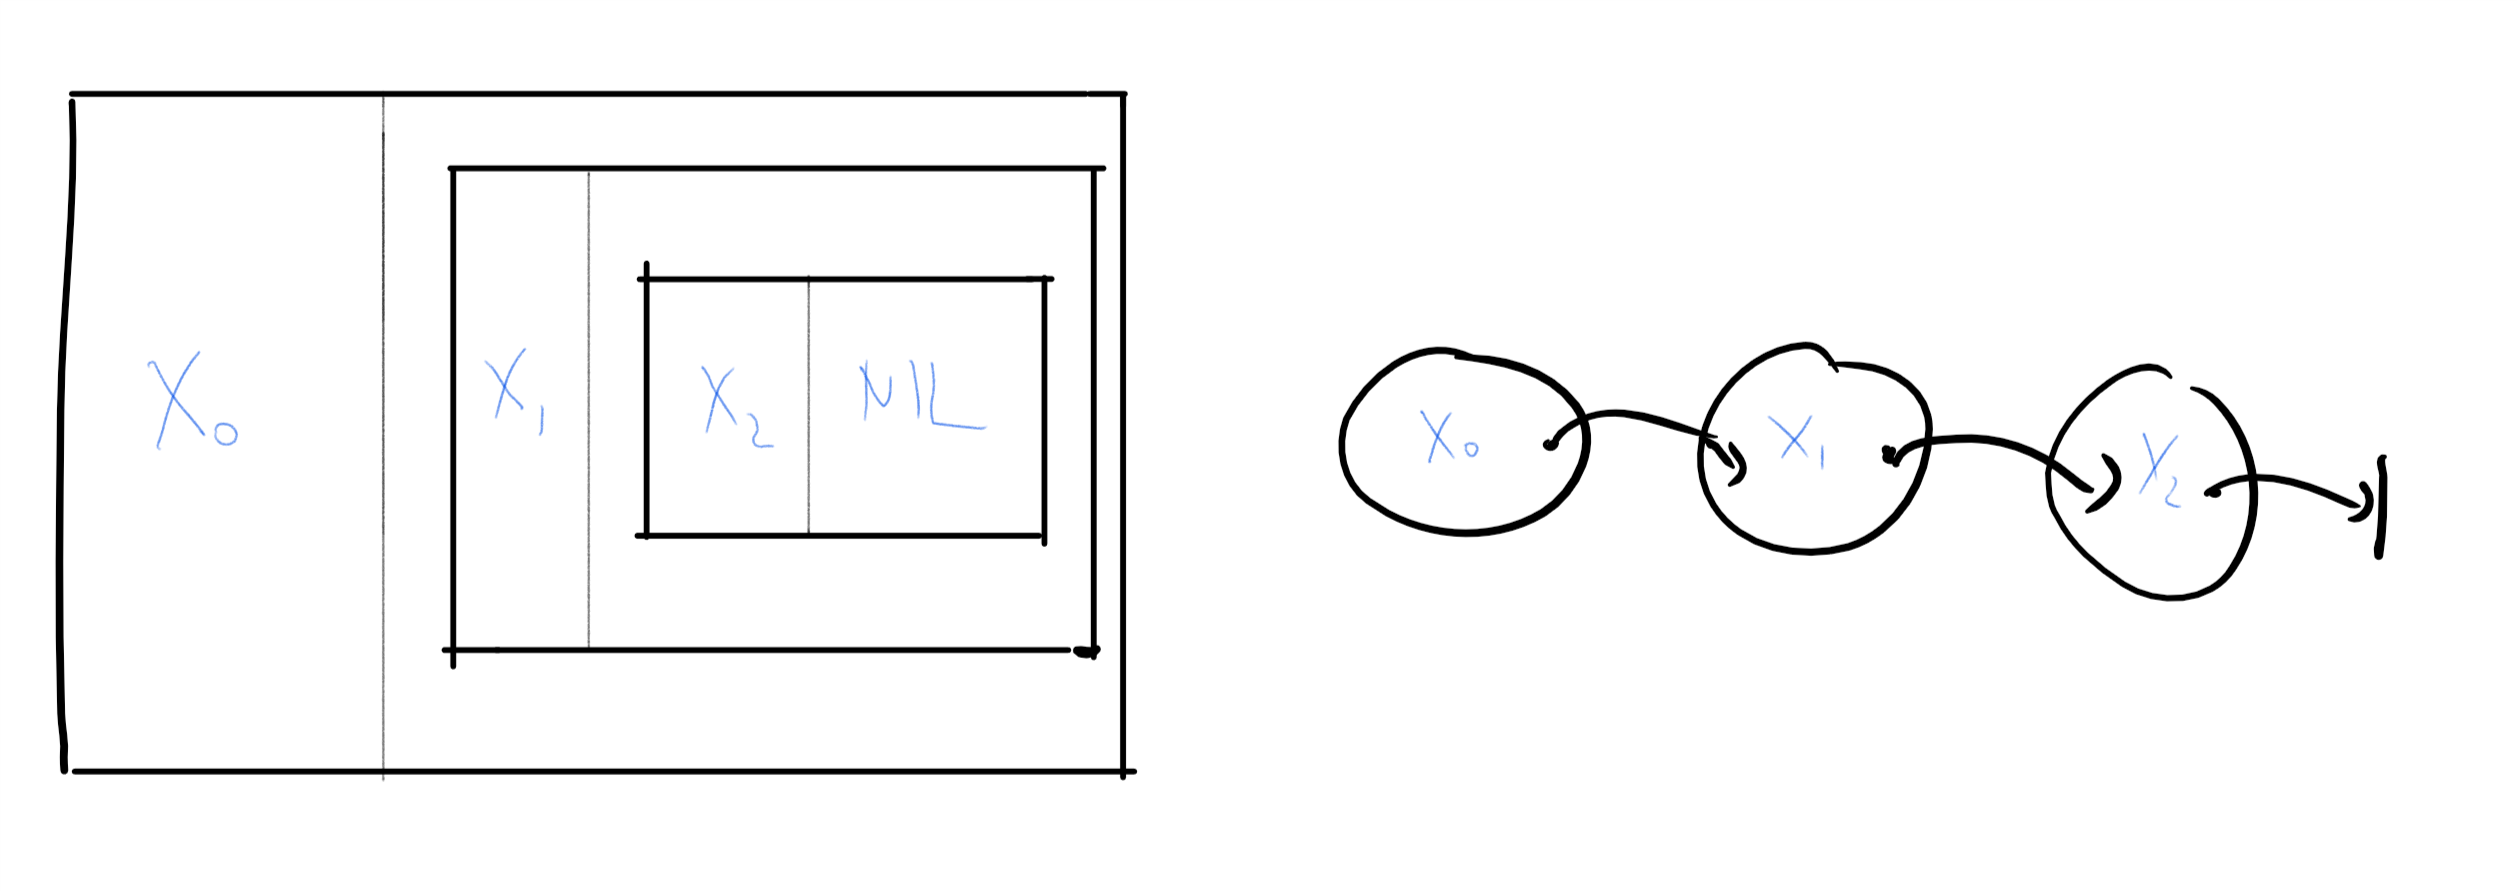
\includegraphics[width=\textwidth, height=0.25\paperheight, keepaspectratio]{../figure/lambdalist.png}
\caption{A list \(\langle x_0,x_1,x_2 \rangle\) in the λ calculus is
constructed from the tail up, building the pair
\(\langle x_2,\ensuremath{\mathit{NIL}}\rangle\), then the pair
\(\langle x_1, \langle x_2,\ensuremath{\mathit{NIL}}\rangle \rangle\)
and finally the pair
\(\langle x_0,\langle x_1,\langle x_2,\ensuremath{\mathit{NIL}} \rangle\rangle\rangle\).
That is, a list is a pair where the first element of the pair is the
first element of the list and the second element is the rest of the
list. The figure on the left renders this ``pairs inside pairs''
construction, though it is often easier to think of a list as a
``chain'', as in the figure on the right, where the second element of
each pair is thought of as a \emph{link}, \emph{pointer} or
\emph{reference} to the remainder of the list.}
\label{lambdalistfig}
\end{figure}


\begin{figure}
\centering
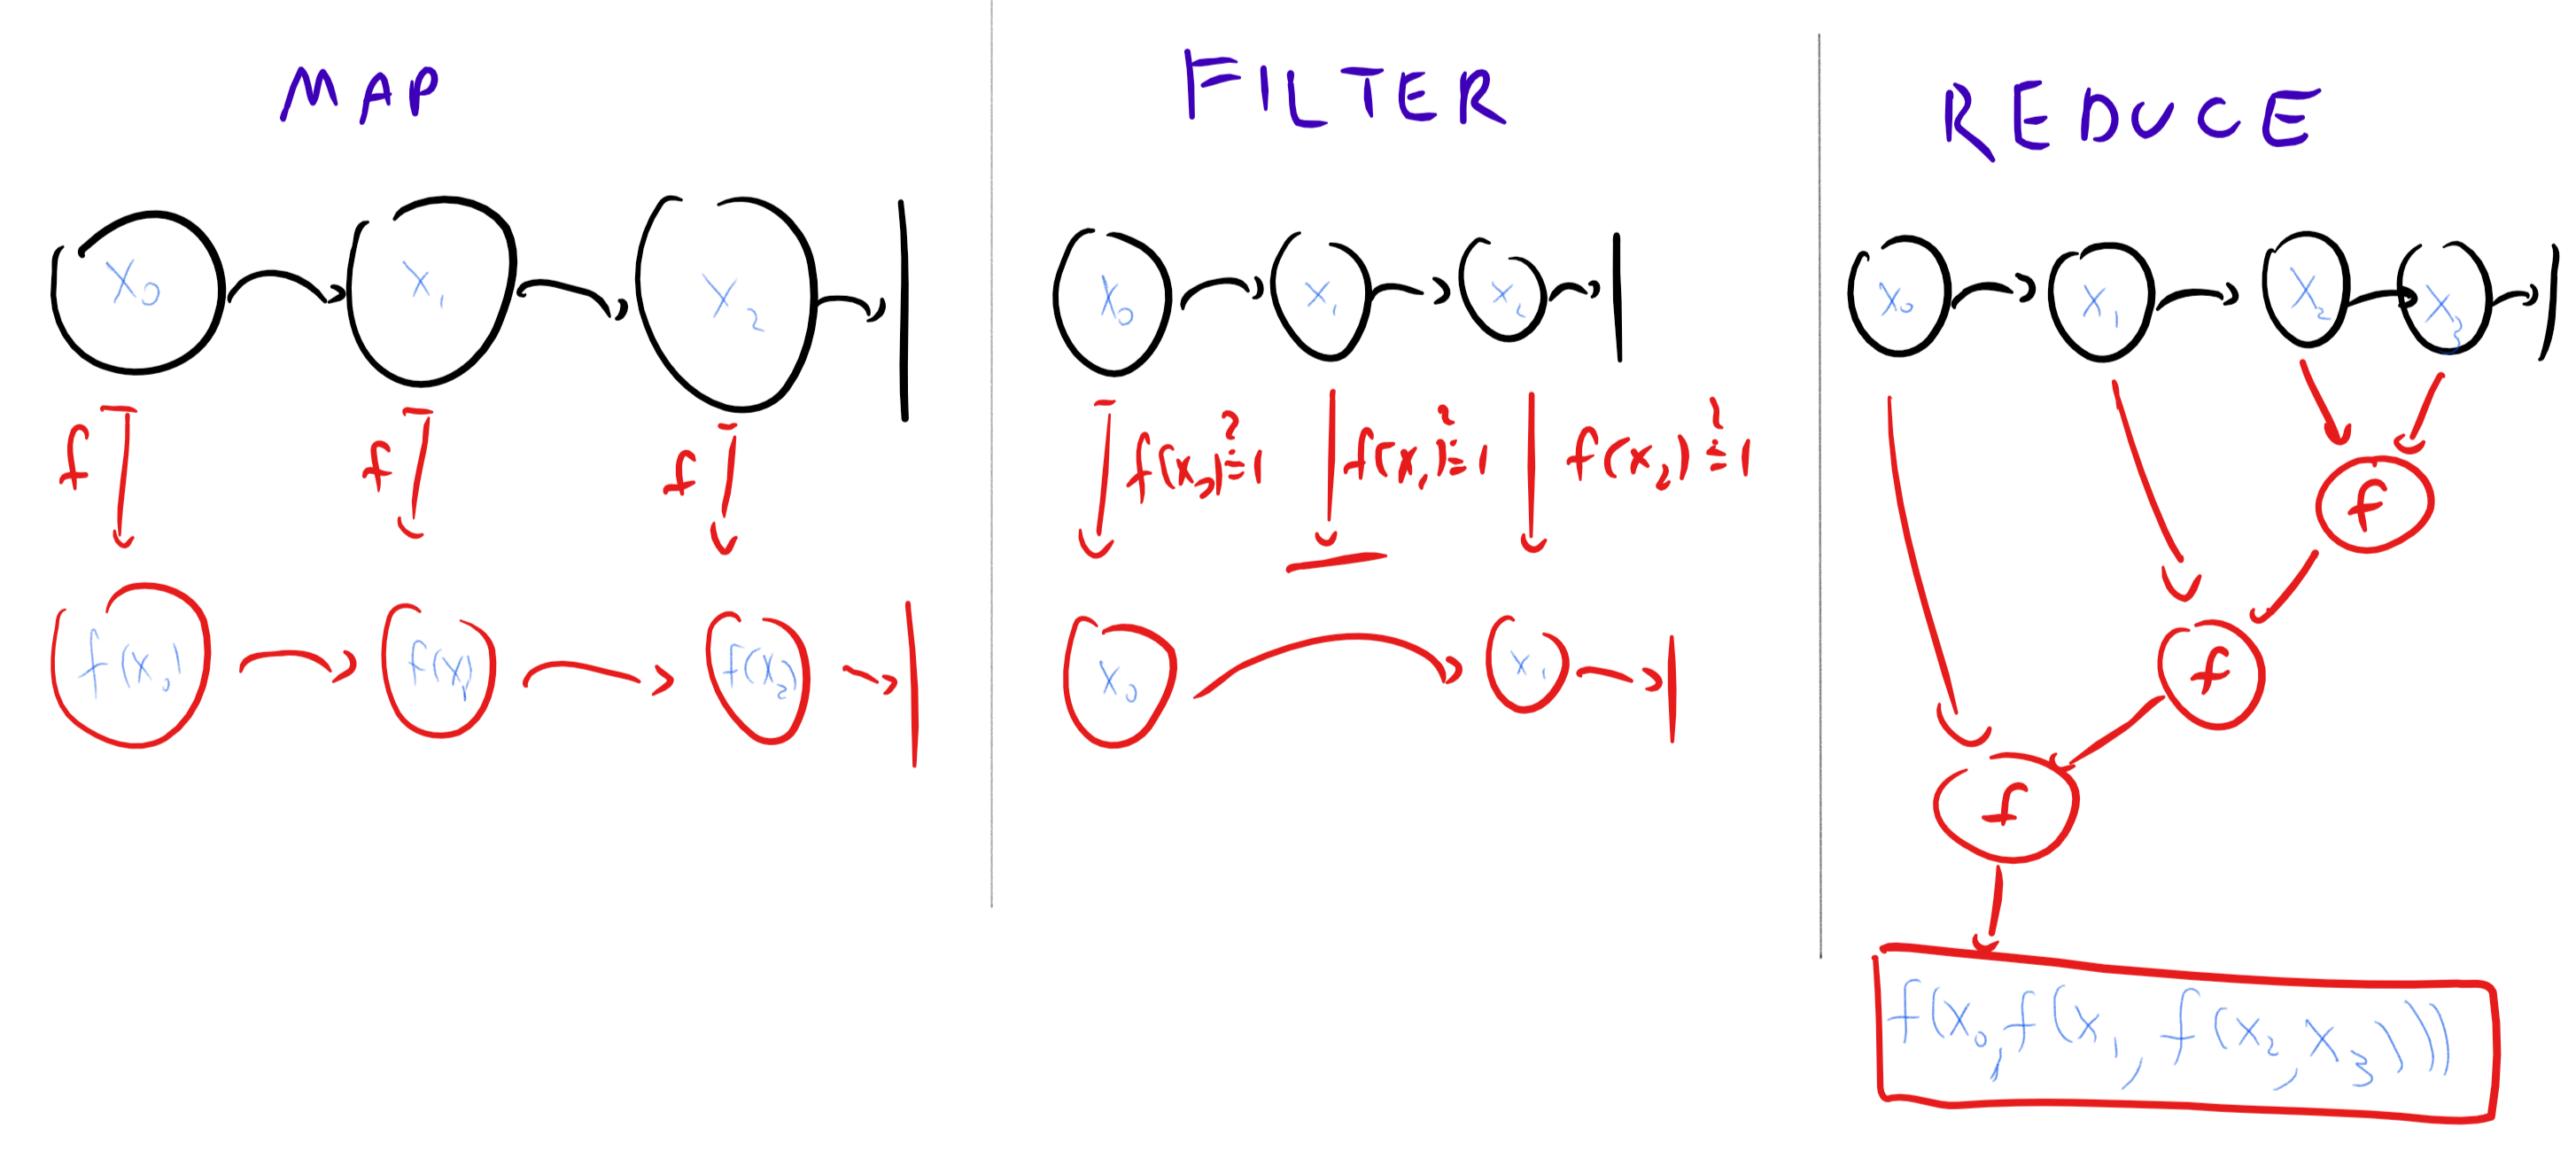
\includegraphics[width=\textwidth, height=0.25\paperheight, keepaspectratio]{../figure/reducemapfilter.png}
\caption{Illustration of the \(\ensuremath{\mathit{MAP}}\),
\(\ensuremath{\mathit{FILTER}}\) and \(\ensuremath{\mathit{REDUCE}}\)
operations.}
\label{reduceetalfig}
\end{figure}

\subsection{Computing a function in the enhanced λ
calculus}\label{Computing-a-function-in-t}

An \emph{enhanced λ expression} is obtained by composing the objects
above with the \emph{application} and \emph{abstraction} rules. The
result of simplifying a λ expression is an equivalent expression, and
hence if two expressions have the same simplification then they are
equivalent.

\hypertarget{lambdacomputedef}{}
\begin{definition}[Computing a function via λ calculus] \label[definition]{lambdacomputedef}

Let \(F:\{0,1\}^* \rightarrow \{0,1\}^*\)

We say that \emph{\(exp\) computes \(F\)} if for every
\(x\in \{0,1\}^*\),

\[exp \langle x_0,\ldots,x_{n-1},\bot \rangle \cong \langle y_0,\ldots, y_{m-1}, \bot \rangle\]

where \(n=|x|\), \(y=F(x)\), and \(m=|y|\), and the notion of
equivalence is defined as per \cref{simplifylambdadef}.

\end{definition}

\subsection{Enhanced λ calculus is
Turing-complete}\label{Enhanced--calculus-is-Tur}

The basic operations of the enhanced λ calculus more or less amount to
the Lisp or Scheme programming languages. Given that, it is perhaps not
surprising that the enhanced λ-calculus is equivalent to Turing
machines:

\hypertarget{lambdaturing-thm}{}
\begin{theorem}[Lambda calculus and NAND-TM] \label[theorem]{lambdaturing-thm}

For every function \(F:\{0,1\}^* \rightarrow \{0,1\}^*\), \(F\) is
computable in the enhanced λ calculus if and only if it is computable by
a Turing machine.

\end{theorem}

\begin{proofidea} \label[proofidea]{To-prove-the-theorem-we-n}

To prove the theorem, we need to show that \textbf{(1)} if \(F\) is
computable by a λ calculus expression then it is computable by a Turing
machine, and \textbf{(2)} if \(F\) is computable by a Turing machine,
then it is computable by an enhanced λ calculus expression.

Showing \textbf{(1)} is fairly straightforward. Applying the
simplification rules to a λ expression basically amounts to ``search and
replace'' which we can implement easily in, say, NAND-RAM, or for that
matter Python (both of which are equivalent to Turing machines in
power). Showing \textbf{(2)} essentially amounts to simulating a Turing
machine (or writing a NAND-TM interpreter) in a functional programming
language such as LISP or Scheme. We give the details below but how this
can be done is a good exercise in mastering some functional programming
techniques that are useful in their own right.

\end{proofidea}

\begin{proof}[Proof of \cref{lambdaturing-thm}] \label[proof]{We-only-sketch-the-proof-}

We only sketch the proof. The ``if'' direction is simple. As mentioned
above, evaluating λ expressions basically amounts to ``search and
replace''. It is also a fairly straightforward programming exercise to
implement all the above basic operations in an imperative language such
as Python or C, and using the same ideas we can do so in NAND-RAM as
well, which we can then transform to a NAND-TM program.

For the ``only if'' direction we need to simulate a Turing machine using
a λ expression. We will do so by first showing that showing for every
Turing machine \(M\) a λ expression to compute the next-step function
\(\ensuremath{\mathit{NEXT}}_M:\overline{\Sigma}^* \rightarrow \overline{\Sigma}^*\)
that maps a configuration of \(M\) to the next one (see
\cref{turingmachinesconfigsec}).

A configuration of \(M\) is a string \(\alpha \in \overline{\Sigma}^*\)
for a finite set \(\overline{\Sigma}\). We can encode every symbol
\(\sigma \in \overline{\Sigma}\) by a finite string \(\{0,1\}^\ell\),
and so we will encode a configuration \(\alpha\) in the λ calculus as a
list \(\langle \alpha_0, \alpha_1, \ldots, \alpha_{m-1}, \bot \rangle\)
where \(\alpha_i\) is an \(\ell\)-length string (i.e., an
\(\ell\)-length list of \(0\)'s and \(1\)'s) encoding a symbol in
\(\overline{\Sigma}\).

By \cref{nextstepfunctionlem}, for every
\(\alpha \in \overline{\Sigma}^*\),
\(\ensuremath{\mathit{NEXT}}_M(\alpha)_i\) is equal to
\(r(\alpha_{i-1},\alpha_i,\alpha_{i+1})\) for some finite function
\(r:\overline{\Sigma}^3 \rightarrow \overline{\Sigma}\). Using our
encoding of \(\overline{\Sigma}\) as \(\{0,1\}^\ell\), we can also think
of \(r\) as mapping \(\{0,1\}^{3\ell}\) to \(\{0,1\}^\ell\). By
\cref{NANDlambdaex}, we can compute the \(\ensuremath{\mathit{NAND}}\)
function, and hence \emph{every} finite function, including \(r\), using
the λ calculus. Using this insight, we can compute
\(\ensuremath{\mathit{NEXT}}_M\) using the λ calculus as follows. Given
a list \(L\) encoding the configuration \(\alpha_0\cdots \alpha_{m-1}\),
we define the lists \(L_{prev}\) and \(L_{next}\) encoding the
configuration \(\alpha\) shifted by one step to the right and left
respectively. The next configuration \(\alpha'\) is defined as
\(\alpha'_i = r(L_{prev}[i],L[i],L_{next}[i])\) where we let \(L'[i]\)
denote the \(i\)-th element of \(L'\). This can be computed by recursion
(and hence using the enhanced λ calculus'
\(\ensuremath{\mathit{RECURSE}}\) operator) as follows:

\begin{algorithm}[$NEXT_M$ using the λ calculus]
\label[algorithm]{nextmlambdacalc} ~ \\ \noindent
\begin{algorithmic}[1]
\INPUT  List $L = \langle \alpha_0,\alpha_1,\ldots, \alpha_{m-1}, \bot \rangle$ encoding a configuration $\alpha$.
\OUTPUT  List $L'$ encoding $NEXT_M(\alpha)$
\PROCEDURE{ComputeNext}{$L_{prev},L,L_{next}$}
\IF $ISEMPTY \; L_{prev}$
\RETURN $NIL$
\ENDIF
\STATE $a \leftarrow HEAD \; L_{prev}$
\IF $ISEMPTY\; L$
\STATE $b \leftarrow \varnothing$ \COMMENT{ Encoding of $\varnothing$ in $\{0,1\}^\ell$}
\ELSE
\STATE $b \leftarrow HEAD\;L$
\ENDIF
\IF $ISEMPTY\; L_{next}$
\STATE $c \leftarrow \varnothing$
\ELSE
\STATE $c \leftarrow HEAD \; L_{next}$
\ENDIF
\RETURN $PAIR \; r(a,b,c) \;$ \CALL{ComputeNext}{$TAIL\; L_{prev}\;,\;TAIL\; L\;,\;TAIL\; L_{next}$} 
\ENDPROCEDURE
\STATE $L_{prev} \leftarrow PAIR \; \varnothing \; L$ \COMMENT{ $L_{prev} = \langle \varnothing , \alpha_0,\ldots, \alpha_{m-1},\bot \rangle$}
\STATE $L_{next} \leftarrow  TAIL\; L$ \COMMENT{ $L_{next} = \langle \alpha_1,\ldots,\alpha_{m-1}, \bot \}$}
\RETURN \CALL{ComputeNext}{$L_{prev},L,L_{next}$} 
\end{algorithmic}
\end{algorithm}

Once we can compute \(\ensuremath{\mathit{NEXT}}_M\), we can simulate
the execution of \(M\) on input \(x\) using the following recursion.
Define \(\ensuremath{\mathit{FINAL}}(\alpha)\) to be the final
configuration of \(M\) when initialized at configuration \(\alpha\). The
function \(\ensuremath{\mathit{FINAL}}\) can be defined recursively as
follows:

\[
\ensuremath{\mathit{FINAL}}(\alpha) = \begin{cases}\alpha & \text{$\alpha$ is halting configuration} \\ \ensuremath{\mathit{NEXT}}_M(\alpha) & \text{otherwise}\end{cases}\;.
\]

Checking whether a configuration is halting (i.e., whether it is one in
which the transition function would output \(\mathsf{H}\)alt) can be
easily implemented in the \(\lambda\) calculus, and hence we can use the
\(\ensuremath{\mathit{RECURSE}}\) to compute
\(\ensuremath{\mathit{FINAL}}\). If we let \(\alpha^0\) be the
\emph{initial configuration} of \(M\) on input \(x\) then we can obtain
the output \(M(x)\) from \(\ensuremath{\mathit{FINAL}}(\alpha^0)\),
hence completing the proof.

\end{proof}

\section{From enhanced to pure λ calculus}\label{lambdacacluluspuresec}

While the collection of ``basic'' functions we allowed for the enhanced
λ calculus is smaller than what's provided by most Lisp dialects, coming
from NAND-TM it still seems a little ``bloated''. Can we make do with
less? In other words, can we find a subset of these basic operations
that can implement the rest?

It turns out that there is in fact a proper subset of the operations of
the enhanced λ calculus that can be used to implement the rest. That
subset is the empty set. That is, we can implement \emph{all} the
operations above using the λ formalism only, even without using \(0\)'s
and \(1\)'s. It's λ's all the way down!

\begin{pause} \label[pause]{This-is-a-good-point-to-p}

This is a good point to pause and think how you would implement these
operations yourself. For example, start by thinking how you could
implement \(\ensuremath{\mathit{MAP}}\) using
\(\ensuremath{\mathit{REDUCE}}\), and then
\(\ensuremath{\mathit{REDUCE}}\) using \(\ensuremath{\mathit{RECURSE}}\)
combined with
\(0,1,\ensuremath{\mathit{IF}},\ensuremath{\mathit{PAIR}},\ensuremath{\mathit{HEAD}},\ensuremath{\mathit{TAIL}},\ensuremath{\mathit{NIL}},\ensuremath{\mathit{ISEMPTY}}\).
You can also \(\ensuremath{\mathit{PAIR}}\),
\(\ensuremath{\mathit{HEAD}}\) and \(\ensuremath{\mathit{TAIL}}\) based
on \(0,1,\ensuremath{\mathit{IF}}\). The most challenging part is to
implement \(\ensuremath{\mathit{RECURSE}}\) using only the operations of
the pure λ calculus.

\end{pause}

\hypertarget{enhancedvanillalambdathm}{}
\begin{theorem}[Enhanced λ calculus equivalent to pure λ calculus.] \label[theorem]{enhancedvanillalambdathm}

There are λ expressions that implement the functions
\(0\),\(1\),\(\ensuremath{\mathit{IF}}\),\(\ensuremath{\mathit{PAIR}}\),
\(\ensuremath{\mathit{HEAD}}\), \(\ensuremath{\mathit{TAIL}}\),
\(\ensuremath{\mathit{NIL}}\), \(\ensuremath{\mathit{ISEMPTY}}\),
\(\ensuremath{\mathit{MAP}}\), \(\ensuremath{\mathit{REDUCE}}\), and
\(\ensuremath{\mathit{RECURSE}}\).

\end{theorem}

The idea behind \cref{enhancedvanillalambdathm} is that we encode \(0\)
and \(1\) themselves as λ expressions, and build things up from there.
This is known as \href{https://goo.gl/QZKM9M}{Church encoding}, as it
was originated by Church in his effort to show that the λ calculus can
be a basis for all computation. We will not write the full formal proof
of \cref{enhancedvanillalambdathm} but outline the ideas involved in it:

\begin{itemize}
\item
  We define \(0\) to be the function that on two inputs \(x,y\) outputs
  \(y\), and \(1\) to be the function that on two inputs \(x,y\) outputs
  \(x\). We use Currying to achieve the effect of two-input functions
  and hence \(0 = \lambda x. \lambda y.y\) and
  \(1 = \lambda x.\lambda y.x\). (This representation scheme is the
  common convention for representing \texttt{false} and \texttt{true}
  but there are many other alternative representations for \(0\) and
  \(1\) that would have worked just as well.)
\item
  The above implementation makes the \(\ensuremath{\mathit{IF}}\)
  function trivial: \(\ensuremath{\mathit{IF}}(cond,a,b)\) is simply
  \(cond \; a\; b\) since \(0ab = b\) and \(1ab = a\). We can write
  \(\ensuremath{\mathit{IF}} = \lambda x.x\) to achieve
  \(\ensuremath{\mathit{IF}}(cond,a,b) = (((\ensuremath{\mathit{IF}} cond) a) b) = cond \; a \; b\).
\item
  To encode a pair \((x,y)\) we will produce a function \(f_{x,y}\) that
  has \(x\) and \(y\) ``in its belly'' and satisfies
  \(f_{x,y}g = g x y\) for every function \(g\). That is,
  \(\ensuremath{\mathit{PAIR}} = \lambda x,y. \left(\lambda g. gxy\right)\).
  We can extract the first element of a pair \(p\) by writing \(p1\) and
  the second element by writing \(p0\), and so
  \(\ensuremath{\mathit{HEAD}} = \lambda p. p1\) and
  \(\ensuremath{\mathit{TAIL}} = \lambda p. p0\).
\item
  We define \(\ensuremath{\mathit{NIL}}\) to be the function that
  ignores its input and always outputs \(1\). That is,
  \(\ensuremath{\mathit{NIL}} = \lambda x.1\). The
  \(\ensuremath{\mathit{ISEMPTY}}\) function checks, given an input
  \(p\), whether we get \(1\) if we apply \(p\) to the function
  \(zero = \lambda x,y.0\) that ignores both its inputs and always
  outputs \(0\). For every valid pair of the form
  \(p = \ensuremath{\mathit{PAIR}} x y\), \(p zero = p x y = 0\) while
  \(\ensuremath{\mathit{NIL}} zero=1\). Formally,
  \(\ensuremath{\mathit{ISEMPTY}} = \lambda p. p (\lambda x,y.0)\).
\end{itemize}

\hypertarget{Churchnumrem}{}
\begin{remark}[Church numerals (optional)] \label[remark]{Churchnumrem}

There is nothing special about Boolean values. You can use similar
tricks to implement \emph{natural numbers} using λ terms. The standard
way to do so is to represent the number \(n\) by the function
\(\ensuremath{\mathit{ITER}}_n\) that on input a function \(f\) outputs
the function \(x \mapsto f(f(\cdots f(x)))\) (\(n\) times). That is, we
represent the natural number \(1\) as \(\lambda f.f\), the number \(2\)
as \(\lambda f.(\lambda x.f(fx))\), the number \(3\) as
\(\lambda f.(\lambda x.f(f(fx)))\), and so on and so forth. (Note that
this is not the same representation we used for \(1\) in the Boolean
context: this is fine; we already know that the same object can be
represented in more than one way.) The number \(0\) is represented by
the function that maps any function \(f\) to the identity function
\(\lambda x.x\). (That is, \(0 = \lambda f.(\lambda x.x)\).)

In this representation, we can compute
\(\ensuremath{\mathit{PLUS}}(n,m)\) as
\(\lambda f.\lambda x.(n f)((m f)x)\) and
\(\ensuremath{\mathit{TIMES}}(n,m)\) as \(\lambda f.n(m f)\).
Subtraction and division are trickier, but can be achieved using
recursion. (Working this out is a great exercise.)

\end{remark}

\subsection{List processing}\label{List-processing}

Now we come to a bigger hurdle, which is how to implement
\(\ensuremath{\mathit{MAP}}\), \(\ensuremath{\mathit{FILTER}}\),
\(\ensuremath{\mathit{REDUCE}}\) and \(\ensuremath{\mathit{RECURSE}}\)
in the pure λ calculus. It turns out that we can build
\(\ensuremath{\mathit{MAP}}\) and \(\ensuremath{\mathit{FILTER}}\) from
\(\ensuremath{\mathit{REDUCE}}\), and \(\ensuremath{\mathit{REDUCE}}\)
from \(\ensuremath{\mathit{RECURSE}}\). For example
\(\ensuremath{\mathit{MAP}}(L,f)\) is the same as
\(\ensuremath{\mathit{REDUCE}}(L,g)\) where \(g\) is the operation that
on input \(x\) and \(y\), outputs
\(\ensuremath{\mathit{PAIR}}(f(x),\ensuremath{\mathit{NIL}})\) if \(y\)
is NIL and otherwise outputs \(\ensuremath{\mathit{PAIR}}(f(x),y)\). (I
leave checking this as a (recommended!) exercise for you, the reader.)

We can define \(\ensuremath{\mathit{REDUCE}}(L,g)\) recursively, by
setting
\(\ensuremath{\mathit{REDUCE}}(\ensuremath{\mathit{NIL}},g)=\ensuremath{\mathit{NIL}}\)
and stipulating that given a non-empty list \(L\), which we can think of
as a pair \((head,rest)\),
\(\ensuremath{\mathit{REDUCE}}(L,g) = g(head, \ensuremath{\mathit{REDUCE}}(rest,g)))\).
Thus, we might try to write a recursive λ expression for
\(\ensuremath{\mathit{REDUCE}}\) as follows

\[
\ensuremath{\mathit{REDUCE}} = \lambda L,g. \ensuremath{\mathit{IF}}(\ensuremath{\mathit{ISEMPTY}}(L),\ensuremath{\mathit{NIL}},g \ensuremath{\mathit{HEAD}}(L) \ensuremath{\mathit{REDUCE}}(\ensuremath{\mathit{TAIL}}(L),g)) \label{reducereceq} \;.
\]

The only fly in this ointment is that the λ calculus does not have the
notion of recursion, and so this is an invalid definition. But of course
we can use our \(\ensuremath{\mathit{RECURSE}}\) operator to solve this
problem. We will replace the recursive call to
``\(\ensuremath{\mathit{REDUCE}}\)'' with a call to a function \(me\)
that is given as an extra argument, and then apply
\(\ensuremath{\mathit{RECURSE}}\) to this. Thus
\(\ensuremath{\mathit{REDUCE}} = \ensuremath{\mathit{RECURSE}}\;myREDUCE\)
where

\[
myREDUCE = \lambda me,L,g. \ensuremath{\mathit{IF}}(\ensuremath{\mathit{ISEMPTY}}(L),\ensuremath{\mathit{NIL}},g \ensuremath{\mathit{HEAD}}(L) me(\ensuremath{\mathit{TAIL}}(L),g)) \label{myreducereceq} \;.
\]

\subsection{The Y combinator, or recursion without
recursion}\label{ycombinatorsec}

\cref{myreducereceq} means that implementing
\(\ensuremath{\mathit{MAP}}\), \(\ensuremath{\mathit{FILTER}}\), and
\(\ensuremath{\mathit{REDUCE}}\) boils down to implementing the
\(\ensuremath{\mathit{RECURSE}}\) operator in the pure λ calculus. This
is what we do now.

How can we implement recursion without recursion? We will illustrate
this using a simple example - the \(\ensuremath{\mathit{XOR}}\)
function. As shown in \cref{XORlambdaex}, we can write the
\(\ensuremath{\mathit{XOR}}\) function of a list recursively as follows:

\[
\ensuremath{\mathit{XOR}}(L) = \begin{cases} 0 & L \text{ is empty} \\ \ensuremath{\mathit{XOR}}_2(\ensuremath{\mathit{HEAD}}(L),\ensuremath{\mathit{XOR}}(\ensuremath{\mathit{TAIL}}(L))) & \text{otherwise}
\end{cases}
\]

where \(\ensuremath{\mathit{XOR}}_2:\{0,1\}^2 \rightarrow \{0,1\}\) is
the XOR on two bits. In \emph{Python} we would write this as

\begin{code}
def xor2(a,b): return 1-b if a else b
def head(L): return L[0]
def tail(L): return L[1:]

def xor(L): return xor2(head(L),xor(tail(L))) if L else 0

print(xor([0,1,1,0,0,1]))
# 1
\end{code}

Now, how could we eliminate this recursive call? The main idea is that
since functions can take other functions as input, it is perfectly legal
in Python (and the λ calculus of course) to give a function
\emph{itself} as input. So, our idea is to try to come up with a
\emph{non recursive} function \texttt{tempxor} that takes \emph{two
inputs}: a function and a list, and such that
\texttt{tempxor(tempxor,L)} will output the XOR of \texttt{L}!

\begin{pause} \label[pause]{At-this-point-you-might-w}

At this point you might want to stop and try to implement this on your
own in Python or any other programming language of your choice (as long
as it allows functions as inputs).

\end{pause}

Our first attempt might be to simply use the idea of replacing the
recursive call by \texttt{me}. Let's define this function as
\texttt{myxor}

\begin{code}
def myxor(me,L): return xor2(head(L),me(tail(L))) if L else 0
\end{code}

Let's test this out:

\begin{code}
myxor(myxor,[1,0,1])
\end{code}

If you do this, you will get the following complaint from the
interpreter:

\texttt{TypeError: myxor() missing 1 required positional argument}

The problem is that \texttt{myxor} expects \emph{two} inputs- a function
and a list- while in the call to \texttt{me} we only provided a list. To
correct this, we modify the call to also provide the function itself:

\begin{code}
def tempxor(me,L): return xor2(head(L),me(me,tail(L))) if L else 0
\end{code}

Note the call \texttt{me(me,..)} in the definition of \texttt{tempxor}:
given a function \texttt{me} as input, \texttt{tempxor} will actually
call the function \texttt{me} with itself as the first input. If we test
this out now, we see that we actually get the right result!

\begin{code}
tempxor(tempxor,[1,0,1])
# 0
tempxor(tempxor,[1,0,1,1])
# 1
\end{code}

and so we can define \texttt{xor(L)} as simply
\texttt{return tempxor(tempxor,L)}.

The approach above is not specific to XOR. Given a recursive function
\texttt{f} that takes an input \texttt{x}, we can obtain a non recursive
version as follows:

\begin{enumerate}
\def\labelenumi{\arabic{enumi}.}
\item
  Create the function \texttt{myf} that takes a pair of inputs
  \texttt{me} and \texttt{x}, and replaces recursive calls to \texttt{f}
  with calls to \texttt{me}.
\item
  Create the function \texttt{tempf} that converts calls in \texttt{myf}
  of the form \texttt{me(x)} to calls of the form \texttt{me(me,x)}.
\item
  The function \texttt{f(x)} will be defined as \texttt{tempf(tempf,x)}
\end{enumerate}

Here is the way we implement the \texttt{RECURSE} operator in Python. It
will take a function \texttt{myf} as above, and replace it with a
function \texttt{g} such that \texttt{g(x)=myf(g,x)} for every
\texttt{x}.

\begin{code}
def RECURSE(myf):
    def tempf(me,x): return myf(lambda y: me(me,y),x)

    return lambda x: tempf(tempf,x)


xor = RECURSE(myxor)

print(xor([0,1,1,0,0,1]))
# 1

print(xor([1,1,0,0,1,1,1,1]))
# 0
\end{code}

\paragraph{From Python to the \lambda calculus.} In the λ calculus, a
two input function \(g\) that takes a pair of inputs \(me,y\) is written
as \(\lambda me.(\lambda y. g)\). So the function \(y \mapsto me(me,y)\)
is simply written as \(me\;me\) and similarly the function
\(x \mapsto tempf(tempf,x)\) is simply \(tempf\; tempf\). (Can you see
why?) Therefore the function \texttt{tempf} defined above can be written
as \texttt{λ me. myf(me me)}. This means that if we denote the input of
\texttt{RECURSE} by \(f\), then
\(\ensuremath{\mathit{RECURSE}}\; myf = tempf \; tempf\) where
\(tempf = \lambda m. f(m\; m)\) or in other words \[
\ensuremath{\mathit{RECURSE}} =  \lambda f.\bigl( (\lambda m. f(m\; m))\;\; (\lambda m. f(m \;m)) \bigr)
\]

The
\href{https://github.com/boazbk/nandnotebooks/blob/master/lambda.ipynb}{online
appendix} contains an implementation of the λ calculus using Python.
Here is an implementation of the recursive XOR function from that
appendix:\footnote{Because of specific issues of Python syntax, in this
  implementation we use \texttt{f * g} for applying \texttt{f} to
  \texttt{g} rather than \texttt{fg}, and use \texttt{λx(exp)} rather
  than \texttt{λx.exp} for abstraction. We also use \texttt{\_0} and
  \texttt{\_1} for the λ terms for \(0\) and \(1\) so as not to confuse
  with the Python constants.}

\begin{code}
# XOR of two bits
XOR2 = λ(a,b)(IF(a,IF(b,_0,_1),b))

# Recursive XOR with recursive calls replaced by m parameter
myXOR = λ(m,l)(IF(ISEMPTY(l),_0,XOR2(HEAD(l),m(TAIL(l)))))

# Recurse operator (aka Y combinator)
RECURSE = λf((λm(f(m*m)))(λm(f(m*m))))

# XOR function
XOR = RECURSE(myXOR)

#TESTING:

XOR(PAIR(_1,NIL)) # List [1]
# equals 1

XOR(PAIR(_1,PAIR(_0,PAIR(_1,NIL)))) # List [1,0,1]
# equals 0
\end{code}

\hypertarget{Ycombinator}{}
\begin{remark}[The Y combinator] \label[remark]{Ycombinator}

The \(\ensuremath{\mathit{RECURSE}}\) operator above is better known as
the
\href{https://en.wikipedia.org/wiki/Fixed-point_combinator\#Fixed_point_combinators_in_lambda_calculus}{Y
combinator}.

It is one of a family of a \emph{fixed point operators} that given a
lambda expression \(F\), find a \emph{fixed point} \(f\) of \(F\) such
that \(f = F f\). If you think about it, \(\ensuremath{\mathit{XOR}}\)
is the fixed point of \(myXOR\) above. \(\ensuremath{\mathit{XOR}}\) is
the function such that for every \(x\), if plug in
\(\ensuremath{\mathit{XOR}}\) as the first argument of \(myXOR\) then we
get back \(\ensuremath{\mathit{XOR}}\), or in other words
\(\ensuremath{\mathit{XOR}} = myXOR\; \ensuremath{\mathit{XOR}}\). Hence
finding a \emph{fixed point} for \(myXOR\) is the same as applying
\(\ensuremath{\mathit{RECURSE}}\) to it.

\end{remark}

\section{The Church-Turing Thesis
(discussion)}\label{churchturingdiscussionsec}

\begin{quote}
\emph{``{[}In 1934{]}, Church had been speculating, and finally
definitely proposed, that the λ-definable functions are all the
effectively calculable functions \ldots. When Church proposed this
thesis, I sat down to disprove it \ldots{} but, quickly realizing that
{[}my approach failed{]}, I became overnight a supporter of the
thesis.''}, Stephen Kleene, 1979.
\end{quote}

\begin{quote}
\emph{``{[}The thesis is{]} not so much a definition or to an axiom but
\ldots{} a natural law.''}, Emil Post, 1936.
\end{quote}

We have defined functions to be \emph{computable} if they can be
computed by a NAND-TM program, and we've seen that the definition would
remain the same if we replaced NAND-TM programs by Python programs,
Turing machines, λ calculus, cellular automata, and many other
computational models. The \emph{Church-Turing thesis} is that this is
the only sensible definition of ``computable'' functions. Unlike the
``Physical Extended Church Turing Thesis'' (PECTT) which we saw before,
the Church Turing thesis does not make a concrete physical prediction
that can be experimentally tested, but it certainly motivates
predictions such as the PECTT. One can think of the Church-Turing Thesis
as either advocating a definitional choice, making some prediction about
all potential computing devices, or suggesting some laws of nature that
constrain the natural world. In Scott Aaronson's words, ``whatever it
is, the Church-Turing thesis can only be regarded as extremely
successful''. No candidate computing device (including quantum
computers, and also much less reasonable models such as the hypothetical
``closed time curve'' computers we mentioned before) has so far mounted
a serious challenge to the Church Turing thesis. These devices might
potentially make some computations more \emph{efficient}, but they do
not change the difference between what is finitely computable and what
is not. (The \emph{extended} Church Turing thesis, which we discuss in
\cref{ECTTsec}, stipulates that Turing machines capture also the limit
of what can be \emph{efficiently} computable. Just like its physical
version, quantum computing presents the main challenge to this thesis.)

\subsection{Different models of
computation}\label{Different-models-of-compu}

We can summarize the models we have seen in the following table:

\begin{longtable}[]{@{}lll@{}}
\caption{Different models for computing finite functions and functions
with arbitrary input length.}\tabularnewline
\toprule
\begin{minipage}[b]{0.31\columnwidth}\raggedright
\textbf{Computational problems}\strut
\end{minipage} & \begin{minipage}[b]{0.27\columnwidth}\raggedright
\textbf{Type of model}\strut
\end{minipage} & \begin{minipage}[b]{0.33\columnwidth}\raggedright
\textbf{Examples}\strut
\end{minipage}\tabularnewline
\midrule
\endfirsthead
\toprule
\begin{minipage}[b]{0.31\columnwidth}\raggedright
\textbf{Computational problems}\strut
\end{minipage} & \begin{minipage}[b]{0.27\columnwidth}\raggedright
\textbf{Type of model}\strut
\end{minipage} & \begin{minipage}[b]{0.33\columnwidth}\raggedright
\textbf{Examples}\strut
\end{minipage}\tabularnewline
\midrule
\endhead
\begin{minipage}[t]{0.31\columnwidth}\raggedright
Finite functions \(f:\{0,1\}^n \rightarrow \{0,1\}^m\)\strut
\end{minipage} & \begin{minipage}[t]{0.27\columnwidth}\raggedright
Non uniform computation (algorithm depends on input length)\strut
\end{minipage} & \begin{minipage}[t]{0.33\columnwidth}\raggedright
Boolean circuits, NAND circuits, straight-line programs (e.g.,
NAND-CIRC)\strut
\end{minipage}\tabularnewline
\begin{minipage}[t]{0.31\columnwidth}\raggedright
Functions with unbounded inputs
\(F:\{0,1\}^* \rightarrow \{0,1\}^*\)\strut
\end{minipage} & \begin{minipage}[t]{0.27\columnwidth}\raggedright
Sequential access to memory\strut
\end{minipage} & \begin{minipage}[t]{0.33\columnwidth}\raggedright
Turing machines, NAND-TM programs\strut
\end{minipage}\tabularnewline
\begin{minipage}[t]{0.31\columnwidth}\raggedright
--\strut
\end{minipage} & \begin{minipage}[t]{0.27\columnwidth}\raggedright
Indexed access / RAM\strut
\end{minipage} & \begin{minipage}[t]{0.33\columnwidth}\raggedright
RAM machines, NAND-RAM, modern programming languages\strut
\end{minipage}\tabularnewline
\begin{minipage}[t]{0.31\columnwidth}\raggedright
--\strut
\end{minipage} & \begin{minipage}[t]{0.27\columnwidth}\raggedright
Other\strut
\end{minipage} & \begin{minipage}[t]{0.33\columnwidth}\raggedright
Lambda calculus, cellular automata\strut
\end{minipage}\tabularnewline
\bottomrule
\end{longtable}

Later on in \cref{spacechap} we will study \emph{memory bounded}
computation. It turns out that NAND-TM programs with a constant amount
of memory are equivalent to the model of \emph{finite automata} (the
adjectives ``deterministic'' or ``nondeterministic'' are sometimes added
as well, this model is also known as \emph{finite state machines}) which
in turn captures the notion of \emph{regular languages} (those that can
be described by
\href{https://en.wikipedia.org/wiki/Regular_expression}{regular
expressions}), which is a concept we will see in \cref{restrictedchap}.

\begin{recap} \label[recap]{While-we-defined-computab}

\begin{itemize}
\tightlist
\item
  While we defined computable functions using Turing machines, we could
  just as well have done so using many other models, including not just
  NAND-TM programs but also RAM machines, NAND-RAM, the λ-calculus,
  cellular automata and many other models.
\item
  Very simple models turn out to be ``Turing complete'' in the sense
  that they can simulate arbitrarily complex computation.
\end{itemize}

\end{recap}

\section{Exercises}\label{Exercises}

\hypertarget{RAMTMalternativeex}{}
\begin{exercise}[Alternative proof for TM/RAM equivalence] \label[exercise]{RAMTMalternativeex}

Let \(\ensuremath{\mathit{SEARCH}}:\{0,1\}^* \rightarrow \{0,1\}^*\) be
the following function. The input is a pair \((L,k)\) where
\(k\in \{0,1\}^*\), \(L\) is an encoding of a list of \emph{key value}
pairs \((k_0,v_1),\ldots,(k_{m-1},v_{m-1})\) where
\(k_0,\ldots,k_{m-1}\), \(v_0,\ldots,v_{m-1}\) are binary strings. The
output is \(v_i\) for the smallest \(i\) such that \(k_i=k\), if such
\(i\) exists, and otherwise the empty string.

\begin{enumerate}
\def\labelenumi{\arabic{enumi}.}
\item
  Prove that \(\ensuremath{\mathit{SEARCH}}\) is computable by a Turing
  machine.
\item
  Let \(\ensuremath{\mathit{UPDATE}}(L,k,v)\) be the function whose
  input is a list \(L\) of pairs, and whose output is the list \(L'\)
  obtained by prepending the pair \((k,v)\) to the beginning of \(L\).
  Prove that \(\ensuremath{\mathit{UPDATE}}\) is computable by a Turing
  machine.
\item
  Suppose we encode the configuration of a NAND-RAM program by a list
  \(L\) of key/value pairs where the key is either the name of a scalar
  variable \texttt{foo} or of the form \texttt{Bar[<num>]} for some
  number \texttt{<num>} and it contains all the nonzero values of
  variables. Let \(\ensuremath{\mathit{NEXT}}(L)\) be the function that
  maps a configuration of a NAND-RAM program at one step to the
  configuration in the next step. Prove that
  \(\ensuremath{\mathit{NEXT}}\) is computable by a Turing machine (you
  don't have to implement each one of the arithmetic operations: it is
  enough to implement addition and multiplication).
\item
  Prove that for every \(F:\{0,1\}^* \rightarrow \{0,1\}^*\) that is
  computable by a NAND-RAM program, \(F\) is computable by a Turing
  machine.
\end{enumerate}

\end{exercise}

\hypertarget{lookup}{}
\begin{exercise}[NAND-TM lookup] \label[exercise]{lookup}

This exercise shows part of the proof that NAND-TM can simulate
NAND-RAM. Produce the code of a NAND-TM program that computes the
function \(\ensuremath{\mathit{LOOKUP}}:\{0,1\}^* \rightarrow \{0,1\}\)
that is defined as follows. On input \(pf(i)x\), where \(pf(i)\) denotes
a prefix-free encoding of an integer \(i\),
\(\ensuremath{\mathit{LOOKUP}}(pf(i)x)=x_i\) if \(i<|x|\) and
\(\ensuremath{\mathit{LOOKUP}}(pf(i)x)=0\) otherwise. (We don't care
what \(\ensuremath{\mathit{LOOKUP}}\) outputs on inputs that are not of
this form.) You can choose any prefix-free encoding of your choice, and
also can use your favorite programming language to produce this code.

\end{exercise}

\hypertarget{pair-ex}{}
\begin{exercise}[Pairing] \label[exercise]{pair-ex}

Let \(embed:\N^2 \rightarrow \N\) be the function defined as
\(embed(x_0,x_1)= \tfrac{1}{2}(x_0+x_1)(x_0+x_1+1) + x_1\).\\

\begin{enumerate}
\def\labelenumi{\arabic{enumi}.}
\item
  Prove that for every \(x^0,x^1 \in \N\), \(embed(x^0,x^1)\) is indeed
  a natural number.\\
\item
  Prove that \(embed\) is one-to-one\\
\item
  Construct a NAND-TM program \(P\) such that for every
  \(x^0,x^1 \in \N\), \(P(pf(x^0)pf(x^1))=pf(embed(x^0,x^1))\), where
  \(pf\) is the prefix-free encoding map defined above. You can use the
  syntactic sugar for inner loops, conditionals, and
  incrementing/decrementing the counter.\\
\item
  Construct NAND-TM programs \(P_0,P_1\) such that for for every
  \(x^0,x^1 \in \N\) and \(i \in N\),
  \(P_i(pf(embed(x^0,x^1)))=pf(x^i)\). You can use the syntactic sugar
  for inner loops, conditionals, and incrementing/decrementing the
  counter.
\end{enumerate}

\end{exercise}

\hypertarget{shortestpathcomputableex}{}
\begin{exercise}[Shortest Path] \label[exercise]{shortestpathcomputableex}

Let \(\ensuremath{\mathit{SHORTPATH}}:\{0,1\}^* \rightarrow \{0,1\}^*\)
be the function that on input a string encoding a triple \((G,u,v)\)
outputs a string encoding \(\infty\) if \(u\) and \(v\) are disconnected
in \(G\) or a string encoding the length \(k\) of the shortest path from
\(u\) to \(v\). Prove that \(\ensuremath{\mathit{SHORTPATH}}\) is
computable by a Turing machine. See footnote for hint.\footnote{You
  don't have to give a full description of a Turing machine: use our
  ``eat the cake and have it too'' paradigm to show the existence of
  such a machine by arguing from more powerful equivalent models.}

\end{exercise}

\hypertarget{longestpathcomputableex}{}
\begin{exercise}[Longest Path] \label[exercise]{longestpathcomputableex}

Let \(\ensuremath{\mathit{LONGPATH}}:\{0,1\}^* \rightarrow \{0,1\}^*\)
be the function that on input a string encoding a triple \((G,u,v)\)
outputs a string encoding \(\infty\) if \(u\) and \(v\) are disconnected
in \(G\) or a string encoding the length \(k\) of the \emph{longest
simple path} from \(u\) to \(v\). Prove that
\(\ensuremath{\mathit{LONGPATH}}\) is computable by a Turing machine.
See footnote for hint.\footnote{Same hint as
  \cref{longestpathcomputableex} applies. Note that for showing that
  \(\ensuremath{\mathit{LONGPATH}}\) is computable you don't have to
  give an \emph{efficient} algorithm.}

\end{exercise}

\hypertarget{shortestpathlambda}{}
\begin{exercise}[Shortest path λ expression] \label[exercise]{shortestpathlambda}

Let \(\ensuremath{\mathit{SHORTPATH}}\) be as in
\cref{shortestpathcomputableex}. Prove that there exists a \(\lambda\)
expression that computes \(\ensuremath{\mathit{SHORTPATH}}\). You can
use \cref{shortestpathcomputableex}

\end{exercise}

\hypertarget{nextstepfunctionlemex}{}
\begin{exercise}[Next-step function is local] \label[exercise]{nextstepfunctionlemex}

Prove \cref{nextstepfunctionlem} and use it to complete the proof of
\cref{onedimcathm}.

\end{exercise}

\hypertarget{lambda-calc-ex}{}
\begin{exercise}[λ calculus requires at most three variables] \label[exercise]{lambda-calc-ex}

Prove that for every λ-expression \(e\) with no free variables there is
an equivalent λ-expression \(f\) that only uses the variables
\(x\),\(y\), and \(z\).\footnote{\textbf{Hint:} You can reduce the
  number of variables a function takes by ``pairing them up''. That is,
  define a λ expression \(\ensuremath{\mathit{PAIR}}\) such that for
  every \(x,y\) \(\ensuremath{\mathit{PAIR}} xy\) is some function \(f\)
  such that \(f0=x\) and \(f1=y\). Then use
  \(\ensuremath{\mathit{PAIR}}\) to iteratively reduce the number of
  variables used.}

\end{exercise}

\hypertarget{evalorderlambdaex}{}
\begin{exercise}[Evaluation order example in λ calculus] \label[exercise]{evalorderlambdaex}

\begin{enumerate}
\def\labelenumi{\arabic{enumi}.}
\item
  Let \(e = \lambda x.7 \left( (\lambda x.xx) (\lambda x.xx) \right)\).
  Prove that the simplification process of \(e\) ends in a definite
  number if we use the ``call by name'' evaluation order while it never
  ends if we use the ``call by value'' order.
\item
  (bonus, challenging) Let \(e\) be any λ expression. Prove that if the
  simplification process ends in a definite number if we use the ``call
  by value'' order then it also ends in such a number if we use the
  ``call by name'' order. See footnote for hint.\footnote{Use structural
    induction on the expression \(e\).}
\end{enumerate}

\end{exercise}

\hypertarget{zipfunctionex}{}
\begin{exercise}[Zip function] \label[exercise]{zipfunctionex}

Give an enhanced λ calculus expression to compute the function \(zip\)
that on input a pair of lists \(I\) and \(L\) of the same length \(n\),
outputs a \emph{list of \(n\) pairs} \(M\) such that the \(j\)-th
element of \(M\) (which we denote by \(M_j\)) is the pair \((I_j,L_j)\).
Thus \(zip\) ``zips together'' these two lists of elements into a single
list of pairs.\footnote{The name \(zip\) is a common name for this
  operation, for example in Python. It should not be confused with the
  \texttt{zip} compression file format.}

\end{exercise}

\hypertarget{lambdaturing-thm}{}
\begin{exercise}[Next-step function without $RECURSE$] \label[exercise]{lambdaturing-thm}

Let \(M\) be a Turing machine. Give an enhanced λ calculus expression to
compute the next-step function \(\ensuremath{\mathit{NEXT}}_M\) of \(M\)
(as in the proof of \cref{lambdaturing-thm}) \emph{without using
\(\ensuremath{\mathit{RECURSE}}\)}. See footnote for hint.\footnote{Use
  \(\ensuremath{\mathit{MAP}}\) and \(\ensuremath{\mathit{REDUCE}}\)
  (and potentially \(\ensuremath{\mathit{FILTER}}\)). You might also
  find the function \(zip\) of \cref{zipfunctionex} useful.}

\end{exercise}

\hypertarget{lambdacompiler}{}
\begin{exercise}[λ calculus to NAND-TM compiler (challenging)] \label[exercise]{lambdacompiler}

Give a program in the programming language of your choice that takes as
input a λ expression \(e\) and outputs a NAND-TM program \(P\) that
computes the same function as \(e\). For partial credit you can use the
\texttt{GOTO} and all NAND-CIRC syntactic sugar in your output program.
You can use any encoding of λ expressions as binary string that is
convenient for you. See footnote for hint.\footnote{Try to set up a
  procedure such that if array \texttt{Left} contains an encoding of a λ
  expression \(\lambda x.e\) and array \texttt{Right} contains an
  encoding of another λ expression \(e'\), then the array
  \texttt{Result} will contain \(e[x \rightarrow e']\).}

\end{exercise}

\hypertarget{altlambdaex}{}
\begin{exercise}[At least two in $\lambda$ calculus] \label[exercise]{altlambdaex}

Let \(1 = \lambda x,y.x\) and \(0 = \lambda x,y.y\) as before. Define

\[
\ensuremath{\mathit{ALT}} = \lambda a,b,c.(a (b 1 (c 1 0)) (b c 0))
\]

Prove that \(\ensuremath{\mathit{ALT}}\) is a \(\lambda\) expression
that computes the \emph{at least two} function. That is, for every
\(a,b,c \in \{0,1\}\) (as encoded above)
\(\ensuremath{\mathit{ALT}} a b c = 1\) if and only at least two of
\(\{a,b,c\}\) are equal to \(1\).

\end{exercise}

\hypertarget{stringsprogramex}{}
\begin{exercise}[Locality of next-step function] \label[exercise]{stringsprogramex}

This question will help you get a better sense of the notion of
\emph{locality of the next step function} of Turing Machines. This
locality plays an important role in results such as the Turing
completeness of \(\lambda\) calculus and one dimensional cellular
automata, as well as results such as Godel's Incompleteness Theorem and
the Cook Levin theorem that we will see later in this course. Define
\texttt{STRINGS} to be the a programming language that has the following
semantics:

\begin{itemize}
\item
  A \texttt{STRINGS} program \(Q\) has a single string variable
  \texttt{str} that is both the input and the output of \(Q\). The
  program has no loops and no other variables, but rather consists of a
  sequence of conditional search and replace operations that modify
  \texttt{str}.
\item
  The operations of a \texttt{STRINGS} program are:

  \begin{itemize}
  \tightlist
  \item
    \texttt{REPLACE(pattern1,pattern2)} where \texttt{pattern1} and
    \texttt{pattern2} are fixed strings. This replaces the first
    occurrence of \texttt{pattern1} in \texttt{str} with
    \texttt{pattern2}
  \item
    \texttt{if search(pattern) \{ code \}} executes \texttt{code} if
    \texttt{pattern} is a substring of \texttt{str}. The code
    \texttt{code} can itself include nested \texttt{if}'s. (One can also
    add an \texttt{else \{ ... \}} to execute if \texttt{pattern} is
    \emph{not} a substring of condf).
  \item
    the returned value is \texttt{str}
  \end{itemize}
\item
  A \texttt{STRING} program \(Q\) computes a function
  \(F:\{0,1\}^* \rightarrow \{0,1\}^*\) if for every \(x\in \{0,1\}^*\),
  if we initialize \texttt{str} to \(x\) and then execute the sequence
  of instructions in \(Q\), then at the end of the execution
  \texttt{str} equals \(F(x)\).
\end{itemize}

For example, the following is a \texttt{STRINGS} program that computes
the function \(F:\{0,1\}^* \rightarrow \{0,1\}^*\) such that for every
\(x\in \{0,1\}^*\), if \(x\) contains a substring of the form
\(y=11ab11\) where \(a,b \in \{0,1\}\), then \(F(x)=x'\) where \(x'\) is
obtained by replacing the first occurrence of \(y\) in \(x\) with
\(00\).

\begin{code}
if search('110011') {
    replace('110011','00')
} else if search('110111') {
    replace('110111','00')
} else if search('111011') {
    replace('111011','00')
} else if search('111111') {
    replace('1111111','00')
}
\end{code}

Prove that for every Turing Machine program \(M\), there exists a
\texttt{STRINGS} program \(Q\) that computes the
\(\ensuremath{\mathit{NEXT}}_M\) function that maps every string
encoding a valid \emph{configuration} of \(M\) to the string encoding
the configuration of the next step of \(M\)'s computation. (We don't
care what the function will do on strings that do not encode a valid
configuration.) You don't have to write the \texttt{STRINGS} program
fully, but you do need to give a convincing argument that such a program
exists.

\end{exercise}

\section{Bibliographical notes}\label{othermodelsbibnotes}

Chapters 7 in the wonderful book of Moore and Mertens
\cite{MooreMertens11} contains a great exposition much of this material.
.

The RAM model can be very useful in studying the concrete complexity of
practical algorithms. Its theoretical study was initiated in
\cite{cook1973time}. However, the exact set of operations that are
allowed in the RAM model and their costs vary between texts and
contexts. One needs to be careful in making such definitions, especially
if the word size grows, as was already shown by Shamir
\cite{shamir1979}. Chapter 3 in Savage's book \cite{Savage1998models}
contains a more formal description of RAM machines, see also the paper
\cite{hagerup1998}. A study of RAM algorithms that are independent of
the input size (known as the ``transdichotomous RAM model'') was
initiated by \cite{fredman1993}

The models of computation we considered so far are inherently
sequential, but these days much computation happens in parallel, whether
using multi-core processors or in massively parallel distributed
computation in data centers or over the Internet. Parallel computing is
important in practice, but it does not really make much difference for
the question of what can and can't be computed. After all, if a
computation can be performed using \(m\) machines in \(t\) time, then it
can be computed by a single machine in time \(mt\).

The λ-calculus was described by Church in \cite{church1941}. Pierce's
book \cite{pierce2002types} is a canonical textbook, see also
\cite{barendregt1984}. The ``Currying technique'' is named after the
logician \href{https://goo.gl/C9hKz1}{Haskell Curry} (the \emph{Haskell}
programming language is named after Haskell Curry as well). Curry
himself attributed this concept to \href{https://goo.gl/qJqd47}{Moses
Schönfinkel}, though for some reason the term ``Schönfinkeling'' never
caught on.

Unlike most programming languages, the pure λ-calculus doesn't have the
notion of \emph{types}. Every object in the λ calculus can also be
thought of as a λ expression and hence as a function that takes one
input and returns one output. All functions take one input and return
one output, and if you feed a function an input of a form it didn't
expect, it still evaluates the λ expression via ``search and replace'',
replacing all instances of its parameter with copies of the input
expression you fed it. Typed variants of the λ calculus are objects of
intense research, and are strongly related to type systems for
programming language and computer-verifiable proof systems, see
\cite{pierce2002types}. Some of the typed variants of the λ calculus do
not have infinite loops, which makes them very useful as ways of
enabling static analysis of programs as well as computer-verifiable
proofs. We will come back to this point in \cref{restrictedchap} and
\cref{chapproofs}.

Tao has
\href{https://terrytao.wordpress.com/2014/02/04/finite-time-blowup-for-an-averaged-three-dimensional-navier-stokes-equation/}{proposed}
showing the Turing completeness of fluid dynamics (a ``water computer'')
as a way of settling the question of the behavior of the Navier-Stokes
equations, see this
\href{https://www.quantamagazine.org/terence-tao-proposes-fluid-new-path-in-navier-stokes-problem-20140224/}{popular
article}.
